\documentclass[11pt]{article}
\IfFileExists{lmodern.sty}{\usepackage[T1]{fontenc}}{}
\usepackage[utf8]{inputenc}
\IfFileExists{lmodern.sty}{\usepackage{lmodern}}{}
\usepackage{amsmath,amssymb,amsthm,mathtools,graphicx}
\usepackage[margin=1in]{geometry}
\PassOptionsToPackage{hyphens}{url}\usepackage{url}
\usepackage[hidelinks]{hyperref}
\usepackage{microtype}
\hypersetup{pdftitle={Exact transport and spectral dimensions for the almost Mathieu operator},pdfauthor={Seth Douglas and Nidhal Mghirbi}}
\newcommand{\C}{\mathbb C}
\newcommand{\N}{\mathbb N}
\newcommand{\Z}{\mathbb Z}
\newcommand{\Q}{\mathbb Q}
\newcommand{\R}{\mathbb R}
\newcommand{\T}{\mathbb T}
\newcommand{\un}{\mathbf 1}
\newcommand{\tr}{\operatorname{tr}}
\newcommand{\ad}{\operatorname{ad}}
\newcommand{\dist}{\operatorname{dist}}
\newcommand{\supp}{\operatorname{supp}}
\newcommand{\Ga}{G_\alpha}
\newcommand{\au}{\alpha_u^+}
\newcommand{\eps}{\varepsilon}
\newtheorem{theorem}{Theorem}[section]
\newtheorem{lemma}[theorem]{Lemma}
\newtheorem{proposition}[theorem]{Proposition}
\newtheorem{corollary}[theorem]{Corollary}
\newtheorem{maintheorem}{Theorem}
\renewcommand{\themaintheorem}{\Alph{maintheorem}}
\newtheorem{maincorollary}[maintheorem]{Corollary}
\theoremstyle{definition}
\newtheorem{definition}[theorem]{Definition}
\newtheorem{remark}[theorem]{Remark}
\setlength{\emergencystretch}{2em}
\raggedbottom
\title{Exact transport and spectral dimensions\\ for the almost Mathieu operator\thanks{The authors developed this work with AI models from more than one developer and take responsibility for every claim. How the work was done is described at the end of the paper.}}
\author{Seth Douglas \and Nidhal Mghirbi}
\date{Version 2.0.0, October 2026}
\begin{document}
\maketitle
\begin{abstract}
For the almost Mathieu operator with coupling $\lambda>1$ and irrational frequency $\alpha$, let $\beta(\alpha)=\limsup_nq_n^{-1}\log q_{n+1}$ and $\gamma=\max\{0,1-\log\lambda/\beta(\alpha)\}$, read as $0$ if $\beta=0$ and $1$ if $\beta=\infty$. For almost every phase, the upper Abel-averaged transport exponent of every positive moment, normalized by its order, the fastest-tail exponent, and both packing dimensions of every nonzero spectral measure equal $\gamma$. For finite $\beta$ the phase set is an explicit set $G_\alpha^*$, invariant under $\theta\mapsto\theta+\alpha$, that allows subexponential decay of $|\sin2\pi q_n\theta|$ along resonant scales; for $\beta=\infty$ the equalities hold at every phase. The lower bounds hold at every phase. Moreover, for fixed $c>h>\log\lambda$, along scales with $b_n=q_n^{-1}\log|q_n\alpha-p_n|^{-1}\ge c$, the Abel-averaged mass beyond distance $Te^{-hq_n}$ from the launch site tends to one, uniformly in the phase, the launch site and $e^{hq_n}\le T\le|q_n\alpha-p_n|^{-1}$; for a packet launched at the origin and fixed $b>0$, $s\in(0,1)$, the instantaneous mass within that distance exceeds $s$ at only $o(T)$ times in $[0,bT]$. For phases in $G_\alpha^*$, and at every phase if $\beta=\infty$, the upper generalized R\'enyi dimensions of orders $0<r<1$ of the single-site spectral measure equal $\gamma$; the lower ones vanish at every phase. For $1<\lambda<e^\beta$ the packing formula replaces the factor two in the bound of Jitomirskaya, Liu and Tcheremchantsev by the sharp factor one. The proof combines an exactly conserved polynomial with elliptic transfer-matrix estimates; its confining barrier holds at every phase. We give explicit finite-time and finite-volume comparison bounds. At coupling $2$ and phase $1/4$, computable frequencies with eventually odd convergent denominators realize exactly the exponents in $[0,1]$ that are right-c.e.\ relative to the halting problem. One computable frequency has exponent of Turing degree $\mathbf0''$ for every computable coupling in $(1,2^{23/12})$, although finite-time predictions at nonzero error tolerance do not determine it.
\end{abstract}



\section{Introduction}\label{sec:intro}

The almost Mathieu operator
\begin{equation}\label{eq:amo}
(H_{\lambda,\alpha,\theta}u)(n)=u(n+1)+u(n-1)+2\lambda\cos\bigl(2\pi(\theta+n\alpha)\bigr)u(n)
\end{equation}
on $\ell^2(\Z)$ is the central model of quasi-periodic spectral theory. Physicists know it as the Aubry--Andr\'e model~\cite{AubryAndre1980}, and it is realized with cold atoms in bichromatic optical lattices~\cite{Roati2008} and with light in quasi-periodic waveguide arrays~\cite{Lahini2009}. Here $\lambda>0$ is the coupling, $\alpha$ is an irrational frequency and $\theta\in\T=\R/\Z$ is a phase. For $\lambda>1$ the Lyapunov exponent on the spectrum equals $\log\lambda>0$~\cite{BourgainJitomirskaya2002}, but positivity alone does not imply localization.

That picture depends on the arithmetic of $\alpha$. Let $p_n/q_n$ be the continued-fraction convergents of $\alpha$ and
\begin{equation}\label{eq:beta}
\beta(\alpha)=\limsup_{n\to\infty}\frac{\log q_{n+1}}{q_n}\in[0,\infty].
\end{equation}
Avila, You and Zhou~\cite{AYZ2017} proved that the supercritical regime splits sharply at $\lambda=e^{\beta(\alpha)}$. For $\lambda>e^{\beta}$ the operator has Anderson localization for almost every phase. For $1<\lambda<e^{\beta}$ the spectrum is purely singular continuous for every phase. Strongly Liouville frequencies, those with $\beta(\alpha)>0$, can therefore destroy localization even though the Lyapunov exponent stays positive.

What does a wave packet do in that window? For almost every phase, we determine every upper Abel-averaged transport moment exponent and both packing dimensions of every nonzero spectral measure; they equal the same number. The matching lower bounds hold at every phase. The word \emph{upper} matters: the exponent describes the largest long-time bursts, not a power law valid at every time.

The main conclusions are easy to separate. First, the competition between $\log\lambda$ and $\beta(\alpha)$ gives an exact upper transport law on the phase set of Theorem~\ref{thm:A}; when $\beta(\alpha)>\log\lambda$, almost all of the Abel-averaged packet reaches the radii and times specified in Theorem~\ref{thm:B}, at every phase. Second, the same law determines packing dimensions under Theorem~\ref{thm:C}'s phase conditions and, for a packet started at one site, the upper generalized R\'enyi dimensions of orders $0<r<1$ under Theorem~\ref{thm:renyi}'s phase conditions. Third, a computable frequency can produce a noncomputable exponent even though finite-time probabilities for computable data remain effectively approximable. This computability degree persists under computable changes of coupling in an interval; at coupling $2$ and phase $1/4$, however, any finite frequency prefix and any nonzero finite-time error tolerance permit every exponent in the class of Theorem~\ref{thm:D}(2).

\subsection{Transport exponents}

Let $\psi_t=e^{-itH}\delta_0$ and average in time with the exponential weight $(2/T)e^{-2t/T}$:
\begin{equation}\label{eq:abel}
a(j,T)=\frac2T\int_0^\infty e^{-2t/T}\,|\langle\delta_j,\psi_t\rangle|^2\,dt,\qquad
P(N,T)=\sum_{|j|>N}a(j,T),\qquad M_p(T)=\sum_{j\in\Z}|j|^p a(j,T).
\end{equation}
$P(N,T)$ is the time-averaged probability of finding the particle beyond distance $N$, and $M_p(T)$ is the averaged $p$-th moment of the position. The upper transport exponents are
\begin{equation}\label{eq:exponents}
\beta^+(p)=\limsup_{T\to\infty}\frac{\log M_p(T)}{p\log T},\qquad
\au=\sup_{p>0}\beta^+(p).
\end{equation}
The quantity $\au$ is the fastest upper exponent of Damanik and Tcheremchantsev~\cite{DT2007}. It sees even polynomially small tails: if $P(T^a,T)$ decays faster than every power of $T$, then $\au\le a$; if $P(T_j^a,T_j)\ge cT_j^{-C}$ for some $c>0$, $C<\infty$ and a sequence $T_j\to\infty$, then $\au\ge a$. Always $0\le\au\le1$, since hopping is bounded.

Two endpoints were known. Damanik and Tcheremchantsev proved $\au=0$ for $\lambda>1$ when $\beta(\alpha)=0$~\cite{DT2007}, and Jitomirskaya and Zhang proved $\au=1$ for every phase when $\beta(\alpha)=\infty$~\cite{JZ2022}. Jitomirskaya and Kr\"uger proved exponential dynamical localization in phase expectation when $\beta(\alpha)$ is sufficiently small, including positive values~\cite{JK2013}, and Bradshaw, de Jong, Liu, Wang, Wang and Yang refined the growth rates for weakly Liouville frequencies with $\beta(\alpha)=0$~\cite{BdJLWWY2025}. In between, Jitomirskaya and Zhang obtained lower bounds of the form $1-C\log\lambda/\beta$, for every moment~\cite{JZ2022}. Haeming refined them, with an explicit constant, a logarithmic loss and one sequence of times common to all phases~\cite{Haeming2025}. Upper bounds on fractal dimensions of spectral measures near the transition were obtained by Jitomirskaya, Liu and Tcheremchantsev~\cite{JLT2025}. The exact value was open.

\subsection{Main results}

For the exact upper law we use an explicit full-measure set of phases. Begin with
\begin{equation}\label{eq:Ga}
\Ga=\bigl\{\theta\in\T:\ |\sin(2\pi q_n\theta)|\ge q_n^{-2}\ \text{for all sufficiently large }n\bigr\}.
\end{equation}
This set has full Lebesgue measure for every irrational $\alpha$ (Lemma~\ref{lem:Ga}). We shall in fact work with the larger set
\begin{equation}\label{eq:Gastar}
\Ga^*=\Bigl\{\theta\in\T:\ \begin{array}{l}
\text{for every }c,\zeta>0\text{ there is }n_0\text{ such that}\\
|\sin(2\pi q_n\theta)|\ge e^{-\zeta q_n}
\text{ whenever }n\ge n_0\text{ and }b_n\ge c
\end{array}\Bigr\}.
\end{equation}
Here $b_n$ is defined in Section~\ref{sec:prelim}; a condition on a finite set of indices is vacuous, so $\Ga^*=\T$ when $\beta(\alpha)=0$. Equivalently, for every $c>0$ such that $b_n\ge c$ for infinitely many $n$, $q_n^{-1}\log|\sin(2\pi q_n\theta)|\to0$ along those $n$, with $\log0=-\infty$. Only scales with $b_n\ge c$ enter, and along them $|\sin(2\pi q_n\theta)|$ may tend to zero at any subexponential rate. The complement of $\Ga^*$ contains the set $\frac12(\Z+\alpha\Z)$ of phases at which $H_{\lambda,\alpha,\theta}$ is reflection symmetric whenever $\beta(\alpha)>0$, in particular $\theta=0$ (Lemma~\ref{lem:Gastar}). Throughout, the number $\max\{0,1-\log\lambda/\beta(\alpha)\}$ is read as $0$ when $\beta(\alpha)=0$ and as $1$ when $\beta(\alpha)=\infty$.

\begin{maintheorem}[The transport law]\label{thm:A}
Let $\lambda>1$ and let $\alpha$ be irrational.
\begin{enumerate}
\item If $\beta(\alpha)<\infty$, then for every $\theta\in\Ga^*$ and every $p>0$,
\[
\beta^+(p)=\au=\max\Bigl\{0,\ 1-\frac{\log\lambda}{\beta(\alpha)}\Bigr\}
\]
for $H_{\lambda,\alpha,\theta}$, where the right side is read as $0$ when $\beta(\alpha)=0$.
Moreover, for every $a>\max\{0,1-\log\lambda/\beta(\alpha)\}$ and every $m>0$, $P(T^a,T)=O(T^{-m})$ as $T\to\infty$.
\item If $\beta(\alpha)=\infty$, then $\beta^+(p)=\au=1$ for every phase and every $p>0$.
\end{enumerate}
The lower bound $\beta^+(p)\ge\max\{0,1-\log\lambda/\beta(\alpha)\}$ in part~1 holds for every phase and every $p>0$.
\end{maintheorem}

Part~2 is due to Jitomirskaya and Zhang~\cite[Corollary~3]{JZ2022}, and the case $\beta(\alpha)=0$ of part~1 to Damanik and Tcheremchantsev~\cite{DT2007}; we include them so that the statement covers every frequency. The new content is part~1 for $0<\beta(\alpha)<\infty$: the upper bound throughout, and the matching lower bound for every moment when $\beta(\alpha)>\log\lambda$. For $0<\beta(\alpha)<\infty$, the lower bound for the fastest exponent $\au$ also holds for a Lipschitz sampling function whose Lyapunov exponent is continuous on a neighborhood of a spectral minimizer, with $\log\lambda$ replaced by that minimum (Theorem~\ref{thm:L}).

For $\beta(\alpha)<\infty$ and $\theta\in\Ga^*$, Theorem~\ref{thm:A} identifies the competition between the localization rate $\log\lambda$ and the arithmetic rate $\beta(\alpha)$. If $0<\beta(\alpha)<\infty$, the common upper exponent is zero for $\lambda\ge e^{\beta(\alpha)}$, including equality, and increases continuously to $1$ as $\lambda\downarrow1$. If $\beta(\alpha)=0$, it is zero for every $\lambda>1$; if $\beta(\alpha)=\infty$, it is $1$ for every $\lambda>1$ and every phase. Thus, at almost every phase, the finite-positive-beta spectral transition of~\cite{AYZ2017} is also a sharp transition for upper transport exponents. Figure~\ref{fig:exponent} plots the law.

\begin{figure}[t]
\centering
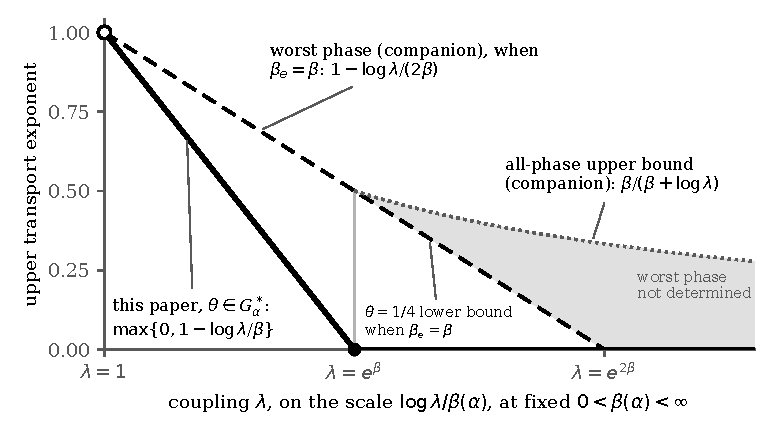
\includegraphics[width=0.8\textwidth]{fig_exponent.pdf}
\caption{The exponent picture: a plot of proved formulas, not of numerical data. At a fixed $0<\beta(\alpha)<\infty$ the horizontal coordinate is $\log\lambda/\beta(\alpha)$, so the marked points are $\lambda=1$, $e^{\beta(\alpha)}$ and $e^{2\beta(\alpha)}$. Solid line: the law of this paper, $\max\{0,1-\log\lambda/\beta(\alpha)\}$, which for $\theta\in G_\alpha^*$ is the common value of every upper Abel-averaged transport exponent and of both packing dimensions of every nonzero spectral measure (Theorems~\ref{thm:A} and~\ref{thm:C}). It is positive for $1<\lambda<e^{\beta(\alpha)}$ and zero at and above the threshold (closed point). The open point denotes the limit $\lambda\downarrow1$; critical coupling is outside the theorems. For comparison, the other curves show fastest-exponent results of the worst-case companion~\cite{DMworstcase}, not of this paper. Dashed: $\max\{0,1-\log\lambda/(2\beta(\alpha))\}$, for frequencies with $\beta_e(\alpha)=\beta(\alpha)$, where $\beta_e$ is the limsup of $b_n$ along even denominators. For $\lambda\le e^{\beta(\alpha)}$ it is then the exponent at the phase $1/4$ and the supremum over all phases; for $\lambda>e^{\beta(\alpha)}$ it is a lower bound at the phase $1/4$. Dotted: the all-phase upper bound $\beta(\alpha)/(\beta(\alpha)+\log\lambda)$ for $\lambda>e^{\beta(\alpha)}$; in the shaded region the worst phase is not determined. At $\beta(\alpha)=0$ the upper exponents vanish for every $\lambda>1$ at every phase, and at $\beta(\alpha)=\infty$ they equal $1$ at every phase. These are upper exponents, not an instantaneous power law, and the zero branch does not assert bounded moments.}
\label{fig:exponent}
\end{figure}

Here is a heuristic for the exponent in the regime $0<\log\lambda<\beta(\alpha)<\infty$. Write $\delta_n=q_n\alpha-p_n$ and $b_n=q_n^{-1}\log|\delta_n|^{-1}$. A shift by $q=q_n$ sites changes the sampling phase by $\delta=\delta_n$, so the nearly periodic potential drifts slowly from block to block. The conserved polynomial constructed below has a diagonal cosine whose phase changes by $\delta$ per lattice site, giving the spatial scale $|\delta|^{-1}$. At such a scale the relevant band velocity is of exponential order $\lambda^{-q}$. Over the resonant time $T=|\delta|^{-1}=e^{b_nq}$, the corresponding distance is of exponential order $T\lambda^{-q}=T^{1-\log\lambda/b_n}$. Taking a subsequence with $b_n\to\beta(\alpha)$ suggests the formula in Theorem~\ref{thm:A}. For phases in $\Ga^*$, that theorem excludes faster polynomial tails at every sufficiently large averaging time. The next theorem shows, at every phase, that the Abel-averaged mass beyond $Te^{-hq_n}$ tends to one in its stated resonant windows, for every fixed $h>\log\lambda$ and $c>h$.

\begin{maintheorem}[Almost all of the packet moves]\label{thm:B}
Let $\lambda>1$ and let $\alpha$ be irrational. Let $h>\log\lambda$ and $c>h$, and assume $b_n\ge c$ for infinitely many $n$. Then
\[
\lim_{\substack{n\to\infty\\ b_n\ge c}}\ \inf_{\theta\in\T}\ \inf_{e^{hq_n}\le T\le|\delta_n|^{-1}}P_\theta\bigl(Te^{-hq_n},T\bigr)=1 ,
\]
where $P_\theta$ is the outside probability for $H_{\lambda,\alpha,\theta}$ and the initial state $\delta_0$. The same holds, uniformly in $j\in\Z$, for the initial state $\delta_j$, with $|k|>Te^{-hq_n}$ replaced by $|k-j|>Te^{-hq_n}$.
\end{maintheorem}

At the resonant time $T=|\delta_n|^{-1}$ the radius in Theorem~\ref{thm:B} is $e^{(b_n-h)q_n}=T^{1-h/b_n}$. For $\beta(\alpha)>\log\lambda$, take scales with $b_n\to\beta(\alpha)$ and then let $h\downarrow\log\lambda$; this gives the lower bound in Theorem~\ref{thm:A} for every positive moment using the same sequence of averaging times. Quantitatively, for fixed $0<\eta\le1/4$, Theorem~\ref{thm:fraction} bounds the outside probability below by
\[
\bigl(1-C_\eta q_ne^{-(h-\log\lambda)q_n/2}\bigr)
\mu^\theta\bigl(\{|\Delta_n|\le2-3\eta\}\bigr),
\]
and the second factor tends uniformly in $\theta$ to $\frac2\pi\arcsin(1-\frac{3\eta}2)$. The estimate discards the spectral mass near the band edges and an error tending to zero; letting $\eta\downarrow0$ after the scale limit gives probability tending to one. For $\theta\in\Ga^*$ and $\beta(\alpha)<\infty$, fix $c>h>\log\lambda$ and $\eps,M>0$. At all sufficiently large scales with $b_n\ge c$, uniformly for $e^{hq_n}\le T\le|\delta_n|^{-1}$,
\[
\sum_{Te^{-hq_n}<|j|\le2e^{\eps q_n}T\lambda^{-q_n}}a(j,T)=1-o(1),
\qquad P(2e^{\eps q_n}T\lambda^{-q_n},T)\le Ce^{-Mq_n}.
\]
Thus every fixed quantile lies at radius $T\lambda^{-q_n}$ within arbitrarily small fixed positive exponential losses in $q_n$ (Remark~\ref{rem:burst}). These conclusions concern Abel averages and do not specify a packet profile or an instantaneous velocity.

The same number governs the spectral measures. For a finite Borel measure $\mu$ on $\R$ and $E\in\R$, the upper local dimension is
\[
d^+_\mu(E)=\limsup_{r\downarrow0}\frac{\log\mu([E-r,E+r])}{\log r}.
\]
The lower and upper packing dimensions $\dim_P^-(\mu)$ and $\dim_P^+(\mu)$ are, respectively, the $\mu$-essential infimum and supremum of $d^+_\mu$. For $\varphi\in\ell^2(\Z)$, let $\mu_\varphi$ be its spectral measure for $H_{\lambda,\alpha,\theta}$:
\[
\mu_\varphi(B)=\langle\varphi,\un_B(H_{\lambda,\alpha,\theta})\varphi\rangle
\qquad(B\subset\R\ \text{Borel}).
\]

\begin{maintheorem}[Packing dimension]\label{thm:C}
Let $\lambda>1$ and let $\alpha$ be irrational.
\begin{enumerate}
\item For every phase $\theta$ and every nonzero $\varphi\in\ell^2(\Z)$, $d^+_{\mu_\varphi}(E)\ge\max\{0,1-\log\lambda/\beta(\alpha)\}$ for $\mu_\varphi$-almost every $E$, with the right side read as $0$ when $\beta(\alpha)=0$ and as $1$ when $\beta(\alpha)=\infty$. In particular $\dim_P^-(\mu_\varphi)$ is at least this number.
\item If $\beta(\alpha)<\infty$ and $\theta\in\Ga^*$, then for every nonzero $\varphi\in\ell^2(\Z)$,
\[
d^+_{\mu_\varphi}(E)=\max\Bigl\{0,\ 1-\frac{\log\lambda}{\beta(\alpha)}\Bigr\}\quad\text{for $\mu_\varphi$-a.e.\ $E$},
\]
so that $\dim_P^-(\mu_\varphi)=\dim_P^+(\mu_\varphi)=\max\{0,1-\log\lambda/\beta(\alpha)\}$, read as $0$ when $\beta(\alpha)=0$.
\end{enumerate}
\end{maintheorem}

When $\beta(\alpha)=\infty$, part~1 gives $d^+_{\mu_\varphi}\ge1$ almost everywhere at every phase. Every finite Borel measure on $\R$ has upper packing dimension at most $1$, since this dimension is the infimum of the packing dimensions of its full-measure Borel sets~\cite[Appendix]{GSB1999}. So all these packing dimensions equal $1$; this endpoint is due to Jitomirskaya and Zhang~\cite[Corollary~3]{JZ2022}.

The set $\Ga^*$ has full measure and is invariant under $\theta\mapsto\theta+\alpha$ (Lemma~\ref{lem:Gastar}). So for this model the fastest-tail exponent, every moment exponent and the packing dimension coincide: if $\beta(\alpha)<\infty$ and $\theta\in\Ga^*$, then for all $p>0$ and all nonzero $\varphi$,
\[
\au=\beta^+(p)=\dim_P^-(\mu_\varphi)=\dim_P^+(\mu_\varphi)=\max\Bigl\{0,\ 1-\frac{\log\lambda}{\beta(\alpha)}\Bigr\}.
\]

For $0<\log\lambda<\beta(\alpha)<\infty$, Jitomirskaya, Liu and Tcheremchantsev proved the upper packing bound $2(1-\log\lambda/\beta(\alpha))$ for every $\alpha$-Diophantine phase, a full-measure set, and noted that the factor $2$ may not be sharp~\cite[Theorem~1.1]{JLT2025}. Theorem~\ref{thm:C} shows that on $\Ga^*$ the sharp factor is $1$, and that the bound is attained: the upper and lower packing dimensions both equal $1-\log\lambda/\beta$. Their phase set and ours are both of full measure, but neither is shown to contain the other. For $\lambda\ge e^{\beta(\alpha)}$ with $\beta(\alpha)<\infty$, their theorem already gives dimension zero at every $\alpha$-Diophantine phase. In the other direction, Jitomirskaya and Zhang proved lower bounds of the form $1-C\log\lambda/\beta$ for packing dimensions~\cite{JZ2022}. Part~1 gives this bound with $C=1$ at every phase, and part~2 shows that $C=1$ cannot be improved.

The upper bound in part~2 follows from Theorem~\ref{thm:A} and the inequality between moment growth and packing dimension of Guarneri and Schulz-Baldes~\cite{GSB1999}, in the form of Barbaroux, Germinet and Tcheremchantsev~\cite{BGT2000}. Part~1 does not follow from transport bounds, since those inequalities go the other way. It comes from a pointwise bound on the resolvent at the resonant scales (Lemma~\ref{lem:localmass}), which the proof of Theorem~\ref{thm:B} also provides.

The last result concerns computability. The exponent in Theorem~\ref{thm:A} is an explicit function of $\beta(\alpha)$, and $\beta(\alpha)$ is an asymptotic quantity of the continued fraction: it can be noncomputable even when $\alpha$ is computable. A real is computable if rational approximations to any prescribed accuracy can be produced by an algorithm. Two reals have the same Turing degree if each can be computed using the other as an oracle. We write $\mathbf0'$ for the halting problem and $\mathbf0''$ for the halting problem with an oracle for $\mathbf0'$. A real $x$ is \emph{right-c.e.\ relative to $\mathbf 0'$} if the set of rationals $r>x$ is computably enumerable relative to the halting problem.

\begin{maintheorem}[Computability]\label{thm:D}
\begin{enumerate}
\item Let $\lambda>1$ be computable, let $\alpha$ be a computable irrational with $\beta(\alpha)<\infty$, and let $\theta\in\Ga^*$ be computable. Then $\au(H_{\lambda,\alpha,\theta})$ is computable from $\beta(\alpha)$. If moreover $\beta(\alpha)>\log\lambda$, then $\au$ and $\beta(\alpha)$ have the same Turing degree.
\item Take $\lambda=2$ and $\theta=1/4$. As $\alpha$ ranges over the computable irrationals whose convergent denominators are eventually odd, $\au(H_{2,\alpha,1/4})$ ranges over exactly the reals in $[0,1]$ that are right-c.e.\ relative to $\mathbf 0'$.
\item There is an explicit computable irrational $\alpha$ such that $\au(H_{2,\alpha,1/4})\in[11/23,1/2]$ has Turing degree $\mathbf 0''$.
\end{enumerate}
\end{maintheorem}

All Hamiltonian data in part~3 are computable: the coupling $2$, the phase $1/4$ and every digit of $\alpha$. Yet the transport exponent of this explicit operator cannot be computed even with an oracle for the halting problem. Undecidability of physical quantities is known for families of Hamiltonians, most prominently the spectral gap of Cubitt, Perez-Garcia and Wolf~\cite{CPGW2015}. Here a single explicit instance of a textbook one-dimensional model has an exponent of exactly known, high Turing degree. Part~2 identifies the exact set of values, the reals that are right-c.e.\ relative to $\mathbf 0'$. All of them are computable from $\mathbf 0''$, and part~3 shows that degree $\mathbf 0''$ is attained.

\subsection{How the proof works}

There are two lower-bound arguments. Section~\ref{sec:lower} treats the fastest exponent under the hypotheses of Theorem~\ref{thm:L}. For the almost Mathieu operator with $0<\log\lambda<\beta(\alpha)<\infty$, choose $\log\lambda<h<\beta(\alpha)$ and a resonant subsequence with $b_n\to\beta(\alpha)$. On a short interval of energies, the complex-energy transfer matrices have norm at most $Ce^{2hq_n}$ over a distance $N_n=e^{(b_n-h)q_n+O(\log q_n)}$, with averaging times $T_n=e^{b_nq_n+O(\log q_n)}$. Parseval's formula then gives a polynomially small Abel-averaged mass beyond $N_n/2$. This suffices for $\au$, but not for the sharp lower bound on each fixed moment. Section~\ref{sec:moments} supplies that bound by proving that almost all of the Abel-averaged mass escapes beyond the radii of Theorem~\ref{thm:B}.

The upper bound is the main work. Its key object is an exactly conserved quantity at each scale. Chambers' formula~\cite{Chambers1965} says that the discriminant of the $p/q$-periodic approximant depends on the phase only through the energy-independent term $-2\lambda^q\cos(2\pi q\theta)$. Combined with the periodic magic formula of Damanik, Killip and Simon~\cite{DKS2010}, this gives a degree-$q$ polynomial $P_q$ with
\[
P_q(H)=V+K,\qquad V(j)=2\lambda^q\cos\bigl(2\pi(q\theta+j\,\delta)\bigr),\qquad \delta=q\alpha-p,
\]
where $K$ has range $q$ (Proposition~\ref{prop:poly}). At every denominator with $|q\alpha-p|\le e^{-cq}$ for a fixed $c>0$, $K$ is exponentially small compared with $\lambda^q$ (Lemma~\ref{lem:sigma}). The operator $P_q(H)$ commutes with $H$ exactly, so no error accumulates in time. Its diagonal $V$ is a cosine of amplitude $2\lambda^q$ that drifts slowly in space. Three estimates are built on it.
\begin{enumerate}
\item \emph{Barriers} (Section~\ref{sec:barriers}). On the spectral subspace where $P_q(H)$ is near its initial value, the monotone part of the drifting cosine acts as a wall. A Sylvester-equation argument bounds the mass that crosses it, at all times. Dividing $P_q(H)$ by the size of $K$ makes this work at every scale where $|q\alpha-p|$ is exponentially small, even where $K$ itself is large.
\item \emph{Exact slow dynamics} (Section~\ref{sec:filters}). At scales with $|q\alpha-p|\le e^{-(\log\lambda+\eta)q}$, smooth filters on the inverse branches of $P_q$ turn the energy into a smooth function of $P_q(H)/\lambda^q$. On each filtered piece the evolution is exactly generated by an operator whose position commutators give an upper velocity bound of order $\lambda^{-q}$, up to arbitrarily small fixed positive exponential losses in $q$, under the scale and sine conditions of Theorem~\ref{thm:window}. The filtered evolution identity holds for every time.
\item \emph{A per-denominator estimate} (Section~\ref{sec:dt}). For every sufficiently large denominator $q_n$, the complex-energy method of Damanik and Tcheremchantsev~\cite{DT2007} bounds the Abel-averaged mass beyond $C_Dq_n$ by $Ce^{-c_D C_Dq_n}+CT^3e^{-\kappa q_n}$. In particular, this mass is exponentially small in $q_n$ for $1\le T\le e^{\kappa_0q_n}$ with any fixed $0<\kappa_0<\kappa/3$.
\end{enumerate}
The final step (Section~\ref{sec:upper}) is a covering argument. For each large time $T$, look at the first denominator $q_j\ge K\log T$. If it is not too large, the per-denominator estimate confines the packet. If it is very large, the preceding denominator has a definite Liouville ratio and $T$ lies in a fixed logarithmic window of that scale, where the barrier and slow-dynamics estimates apply. No assumption on how the ratios $\log q_{n+1}/q_n$ behave between these scales is needed (Figure~\ref{fig:covering}).

The bulk lower bound in Section~\ref{sec:moments} uses the conserved polynomial again, at scales with $b_n\ge c>h>\log\lambda$. Near the origin, $P_q(H)-2\lambda^q\cos(2\pi q\theta)$ approximates $S^q+S^{-q}$, whose powers have diagonal matrix elements equal to the moments of the arcsine law on $[-2,2]$. The image of the single-site spectral measure under the rational discriminant therefore converges to that law, uniformly in the phase (Lemma~\ref{lem:arcsine}). After excluding a small spectral mass near the band edges, the first $q$-blocks on both sides are elliptic with a definite margin. The resolvent column, restricted to either half-line, is the square-summable solution there, called the Weyl solution. For $e^{hq}\le T\le|\delta|^{-1}$ it remains spread over a long run of consecutive blocks. A pair inequality prevents any polarization from avoiding two adjacent blocks (Lemma~\ref{lem:run}). Comparing the few near blocks with the far mass shows that the mass within $Te^{-hq}$ is negligible. Parseval's formula and Poisson smoothing convert this comparison into Abel-averaged outside probability tending to one, after the band-edge tolerance is sent to zero. At $T=|\delta|^{-1}$, the same runs bound the diagonal resolvent and hence the spectral mass in intervals of radius $|\delta|$, giving the lower bound on upper local dimensions.

\subsection{Organization}

Section~\ref{sec:prelim} fixes notation and collects elementary facts. Section~\ref{sec:poly} constructs the conserved polynomial. Section~\ref{sec:barriers} proves the barrier estimates and Section~\ref{sec:filters} the window theorem for slow dynamics. Section~\ref{sec:dt} records the per-denominator estimate. Section~\ref{sec:upper} proves the upper bound in Theorem~\ref{thm:A}, and Section~\ref{sec:lower} a lower bound for $\au$ that holds for Lipschitz potentials. Section~\ref{sec:moments} proves the bulk lower bound, in which the escaping fraction of the Abel-averaged packet tends to one, and completes the proofs of Theorems~\ref{thm:A}, \ref{thm:B} and~\ref{thm:C}. Section~\ref{sec:renyi} determines generalized R\'enyi dimensions of orders between zero and one. Section~\ref{sec:consequences} proves Theorem~\ref{thm:D} and its coupling and frequency consequences. Section~\ref{sec:finitetime} gives transport at individual times and explicit finite-volume error bounds. Section~\ref{sec:discussion} discusses what remains open.


\section{Preliminaries}\label{sec:prelim}

\subsection{Notation}

Throughout, $\lambda>1$ is fixed, $L=\log\lambda>0$, $v(x)=2\lambda\cos(2\pi x)$, and $H=H_{\lambda,\alpha,\theta}$ is the operator~\eqref{eq:amo}. We write $S$ for the shift $(Su)(n)=u(n+1)$, $X$ for the position operator $X\delta_j=j\delta_j$, and $\un_A$ for multiplication by the indicator of $A\subset\Z$. For a frequency $\omega\in\R$ and a phase $\varphi$ we also use $H_{\lambda,\omega,\varphi}$ with $\omega$ rational. The spectrum $\Sigma$ of $H_{\lambda,\alpha,\theta}$ does not depend on $\theta$ when $\alpha$ is irrational, since lattice translations conjugate $H_{\lambda,\alpha,\theta}$ to $H_{\lambda,\alpha,\theta+k\alpha}$, the orbit $\theta+k\alpha$ is dense, and the operator depends norm-continuously on the phase.

\emph{Transfer matrices.} For $E\in\C$ and $x\in\T$ put $T(E,x)=\begin{pmatrix}E-v(x)&-1\\1&0\end{pmatrix}$ and, for $r\ge0$,
\[
A_r(E,x)=T(E,x+(r-1)\alpha)\cdots T(E,x),\qquad A_0=I.
\]
A solution of $Hu=Eu$ satisfies $(u(r),u(r-1))^{\mathsf T}=A_r(E,\theta)(u(0),u(-1))^{\mathsf T}$. For a frequency $\omega$ other than $\alpha$ we write $A_r^{(\omega)}$. The Lyapunov exponent is $L(E)=\lim_r r^{-1}\int_\T\log\|A_r(E,x)\|\,dx=\inf_r r^{-1}\int_\T\log\|A_r(E,x)\|\,dx$. For $\lambda>1$ it equals $L=\log\lambda$ at every $E\in\Sigma$~\cite[Corollary~2]{BourgainJitomirskaya2002}.

\emph{Continued fractions.} Let $p_n/q_n$ be the convergents of $\alpha$ and put
\[
\delta_n=q_n\alpha-p_n,\qquad D_n=|\delta_n|^{-1},\qquad \beta_n=\frac{\log q_{n+1}}{q_n},\qquad b_n=\frac{\log D_n}{q_n}.
\]
The classical inequalities $(q_{n+1}+q_n)^{-1}<|\delta_n|<q_{n+1}^{-1}$ give
\begin{equation}\label{eq:bn}
q_{n+1}<D_n<2q_{n+1},\qquad 0<b_n-\beta_n<\frac{\log2}{q_n}.
\end{equation}
In particular $\limsup b_n=\limsup\beta_n=\beta(\alpha)$. Denominators grow at least like Fibonacci numbers, and $|\alpha-p_n/q_n|<q_n^{-2}$. When the scale $n$ is fixed we drop the index and write $q,p,\delta,b$, and $A=\lambda^q$. We also write $s=|\sin(2\pi q\theta)|$.

All constants below may depend on $\lambda$, on $\alpha$ and on parameters that are explicitly fixed. They never depend on the phase $\theta$, the scale $n$ or the time $T$, unless this is indicated. Thresholds of the form ``for all sufficiently large $n$'' are likewise uniform in the phase in Sections~\ref{sec:poly}--\ref{sec:dt}, among phases satisfying the stated sine condition at that scale. In Section~\ref{sec:upper} the phase is fixed and thresholds may depend on it.

\subsection{The phase set}

\begin{lemma}\label{lem:Ga}
For every irrational $\alpha$ the set $\Ga$ in~\eqref{eq:Ga} has full Lebesgue measure.
\end{lemma}

\begin{proof}
The map $\theta\mapsto q_n\theta$ preserves Lebesgue measure on $\T$, and $\{x\in\T:|\sin 2\pi x|<u\}$ has measure at most $u$. Hence $\{\theta:|\sin 2\pi q_n\theta|<q_n^{-2}\}$ has measure at most $q_n^{-2}$. Since $\sum_nq_n^{-2}<\infty$, the Borel--Cantelli lemma shows that almost every $\theta$ lies in only finitely many of these sets.
\end{proof}

\subsection{Moments}

\begin{lemma}\label{lem:moments}
\begin{enumerate}
\item For every $p>0$ there is $C_p$, depending only on $p$, such that $M_p(T)\le C_p(1+T)^p$ for all $T>0$ and every bounded potential.
\item For $0<a<1$ and $T\ge1$, $M_p(T)\le T^{ap}+\bigl(M_{2p}(T)\,P(T^a,T)\bigr)^{1/2}$.
\item If $0<a<1$ and $P(T^a,T)=O(T^{-m})$ for every $m>0$, then $\au\le a$.
\end{enumerate}
\end{lemma}

\begin{proof}
1. Let $k\ge1$ be an integer. We have $[X,H]=S^{-1}-S$ and $[X^k,H]=\sum_{i=0}^{k-1}X^{i}[X,H]X^{k-1-i}$. Moving the shifts to the right with $S^{\pm1}X=(X\pm1)S^{\pm1}$ writes $[X^k,H]$ as $\sum_{\pm}c_\pm(X)S^{\pm1}$, where $c_\pm$ are polynomials of degree at most $k-1$ with coefficients bounded by a constant depending only on $k$. Since $X\delta_0=0$, Duhamel's formula $X^k\psi_t=-i\int_0^te^{-i(t-s)H}[X^k,H]\psi_s\,ds$ and induction on $k$ give $\|X^k\psi_t\|\le C_k(1+|t|)^k$. For real $p>0$ choose an integer $k$ with $2k\ge p$. Jensen's inequality for the probability distribution $|\psi_t(j)|^2$ gives
\[
\sum_j|j|^p|\psi_t(j)|^2\le\Bigl(\sum_j|j|^{2k}|\psi_t(j)|^2\Bigr)^{p/(2k)}=\|X^k\psi_t\|^{p/k}\le C(1+|t|)^p.
\] Averaging against $(2/T)e^{-2t/T}$ proves the claim.

2. Split $M_p(T)$ into $|j|\le T^a$ and $|j|>T^a$. The first part is at most $T^{ap}$, because $\sum_ja(j,T)=1$. Apply the Cauchy--Schwarz inequality to the second part, for the probability measure $a(\cdot,T)$ on $\Z$.

3. By parts 1 and 2, $M_p(T)\le T^{ap}+C(1+T)^{p}T^{-m/2}$. Taking $m\ge2p$ gives $M_p(T)\le CT^{ap}$, so $\beta^+(p)\le a$ for every $p$.
\end{proof}

\subsection{Uniform growth near the spectrum}

\begin{lemma}\label{lem:growth}
For every $h>L$ there are a bounded open set $U_h\supset\Sigma$ and a constant $C_h$ such that
\[
\|A_r(E,x)\|\le C_he^{hr}\qquad\text{for all real }E\in U_h,\ x\in\T,\ r\ge0.
\]
\end{lemma}

\begin{proof}
Fix $E_0\in\Sigma$ and $h_1=(L+h)/2$. Since $L(E_0)=L<h_1$, there is $r_0$ with
\[
\frac1{r_0}\int_\T\log\|A_{r_0}(E_0,x)\|\,dx<h_1.
\] The function $F_E(x)=\log\|A_{r_0}(E,x)\|$ is jointly continuous, so the same strict inequality holds for $E$ in a compact neighborhood $N_0$ of $E_0$. Rotation by $r_0\alpha$ is uniquely ergodic, so Birkhoff averages of the continuous functions $F_E$ converge to $\int F_E$ uniformly in $x$; by equicontinuity of $\{F_E\}_{E\in N_0}$ they converge uniformly in $E\in N_0$ as well. Hence there is $m_0$ with $\sum_{k<m}F_E(x+kr_0\alpha)\le mr_0h$ for all $m\ge m_0$, $x\in\T$ and $E\in N_0$. Writing a product of length $r=mr_0+s$ with $0\le s<r_0$ as $m$ blocks of length $r_0$ and a remainder, submultiplicativity gives $\|A_r(E,x)\|\le C e^{hr}$ on $N_0$. A finite cover of the compact set $\Sigma$ by the interiors of such neighborhoods gives $U_h$ and $C_h$.
\end{proof}

\subsection{Rational spectra}

For a rational $p/q$ in lowest terms let $\Sigma_{p/q}=\bigcup_{\varphi\in\T}\sigma(H_{\lambda,p/q,\varphi})$.

\begin{lemma}\label{lem:window}
Let $H_0$ be a bounded Schr\"odinger operator on $\ell^2(\Z)$ with hopping one and real potential, and let $E\in\sigma(H_0)$. For every integer $M\ge1$ there is a unit vector $u$ supported in an interval of length $2M$ with $\|(H_0-E)u\|\le 8/M$.
\end{lemma}

\begin{proof}
By Weyl's criterion there is a finitely supported vector $w$ with $\|(H_0-E)w\|\le M^{-1}\|w\|$. For $k\in\Z$ let $\chi_k(n)=\sin\bigl(\pi(n-kM)/(2M)\bigr)$ for $kM\le n\le (k+2)M$ and $\chi_k(n)=0$ otherwise. Then $\sum_k\chi_k(n)^2=1$, because on $[kM,(k+1)M]$ the two windows $\chi_k$ and $\chi_{k-1}$ are a sine and a cosine of the same angle. Also $|\chi_k(n+1)-\chi_k(n)|\le\pi/(2M)$, and for each $n$ at most three indices $k$ have $\chi_k(n)$ or $\chi_k(n+1)$ nonzero. Since $([S,\chi_k]w)(n)=(\chi_k(n+1)-\chi_k(n))w(n+1)$, this gives $\sum_k\|[S^{\pm1},\chi_k]w\|^2\le 3\pi^2(4M^2)^{-1}\|w\|^2$. Hence $\sum_k\|\chi_kw\|^2=\|w\|^2$ and
\[
\sum_k\|(H_0-E)\chi_kw\|^2\le2\sum_k\|\chi_k(H_0-E)w\|^2+2\sum_k\|[H_0,\chi_k]w\|^2\le\frac{2+6\pi^2}{M^2}\,\|w\|^2.
\]
Some $k$ therefore has $\|(H_0-E)\chi_kw\|\le (8/M)\|\chi_kw\|$.
\end{proof}

\begin{lemma}\label{lem:ratspec}
There is $C$ such that for every rational $p/q$:
\begin{enumerate}
\item every point of $\Sigma_{p/q}$ is within $C|\alpha-p/q|^{1/2}$ of $\Sigma$, and every point of $\Sigma$ is within $C|\alpha-p/q|^{1/2}$ of $\Sigma_{p/q}$;
\item for every $\varphi$, every point of $\Sigma_{p/q}$ is within $2\pi\lambda/q$ of $\sigma(H_{\lambda,p/q,\varphi})$.
\end{enumerate}
\end{lemma}

\begin{proof}
1. Let $E\in\sigma(H_{\lambda,p/q,\varphi})$ and take $u$ from Lemma~\ref{lem:window}, supported in $[c-M,c+M]$. Choose $\theta'$ with $\theta'+c\alpha=\varphi+cp/q$. For $|n-c|\le M$ the potentials of $H_{\lambda,\alpha,\theta'}$ and $H_{\lambda,p/q,\varphi}$ differ by at most $4\pi\lambda M|\alpha-p/q|$. Hence $\dist(E,\Sigma)\le 8/M+4\pi\lambda M|\alpha-p/q|$, and $M=\lceil|\alpha-p/q|^{-1/2}\rceil$ gives the first claim. The second claim is proved in the same way with the roles exchanged.

2. Translation by $k$ sites conjugates $H_{\lambda,p/q,\varphi}$ to $H_{\lambda,p/q,\varphi+kp/q}$, and $\{kp/q\}$ is the full grid $q^{-1}\Z/\Z$. Every phase $\varphi'$ is within $1/(2q)$ of a grid translate of $\varphi$, and the potential is $4\pi\lambda$-Lipschitz in the phase.
\end{proof}

\section{The conserved polynomial}\label{sec:poly}

\subsection{Rational input}

For a rational $p/q$ in lowest terms, the operator $H_{\lambda,p/q,\varphi}$ is $q$-periodic. Its discriminant is $\Delta_\varphi(E)=\tr A^{(p/q)}_q(E,\varphi)$, and its spectrum is $\{E:|\Delta_\varphi(E)|\le2\}$.

\begin{lemma}[Chambers' formula~\cite{Chambers1965}]\label{lem:chambers}
There is a real monic polynomial $P_{p/q}$ of degree $q$ such that
\[
\Delta_\varphi(E)=P_{p/q}(E)-2\lambda^q\cos(2\pi q\varphi)\qquad\text{for all }E\in\C,\ \varphi\in\T.
\]
\end{lemma}

\begin{proof}
Each factor $T(E,\varphi+kp/q)$ is a trigonometric polynomial of degree one in $\varphi$, so $\Delta_\varphi(E)$ is a trigonometric polynomial of degree at most $q$ in $\varphi$. The shift $\varphi\mapsto\varphi+p/q$ cyclically permutes the factors and leaves the trace unchanged. Since $\gcd(p,q)=1$, the trace is invariant under $\varphi\mapsto\varphi+1/q$, so only the Fourier modes $0$ and $\pm q$ survive. The coefficient of $e^{2\pi iq\varphi}$ comes only from the product of the diagonal entries and equals $(-\lambda)^q e^{2\pi i p\,q(q-1)/(2q)}=(-1)^{q+p(q-1)}\lambda^q$. This is $-\lambda^q$ in all cases: if $q$ is odd then $(-1)^{q}=-1$ and $p(q-1)$ is even, and if $q$ is even then $p$ is odd and $(-1)^{p(q-1)}=-1$. The coefficient of $e^{-2\pi iq\varphi}$ is its complex conjugate. The constant mode is a monic polynomial of degree $q$ in $E$ with real coefficients.
\end{proof}

\begin{lemma}[Periodic magic formula~\cite{DKS2010}]\label{lem:magic}
Let $H_{\mathrm{per}}$ be a $q$-periodic Schr\"odinger operator on $\ell^2(\Z)$ with hopping one and discriminant $\Delta$. Then $\Delta(H_{\mathrm{per}})=S^q+S^{-q}$.
\end{lemma}

This is the elementary direction of~\cite[Theorem~3.1]{DKS2010}, proved there by Floquet decomposition (equations (3.5)--(3.6)). The hypotheses hold: the operator is bounded, two-sided, periodic and has positive off-diagonal entries. Combining the two lemmas,
\begin{equation}\label{eq:ratmagic}
P_{p/q}(H_{\lambda,p/q,\varphi})=S^q+S^{-q}+2\lambda^q\cos(2\pi q\varphi).
\end{equation}

\subsection{The irrational operator}

\begin{proposition}\label{prop:poly}
Fix $h>L$. There is $C_h$ such that for all sufficiently large $n$ and every phase $\theta$ the following holds, with $q=q_n$, $p=p_n$, $\delta=\delta_n$ and $P_q=P_{p/q}$.
\begin{enumerate}
\item The operator $Q=P_q(H_{\lambda,\alpha,\theta})$ commutes with $H_{\lambda,\alpha,\theta}$ and decomposes as
\[
Q=V+K,\qquad V(j)=2\lambda^q\cos\bigl(2\pi(q\theta+j\delta)\bigr),\qquad K=S^q+S^{-q}+R,
\]
where $V$ is diagonal, $R$ is self-adjoint, $\langle\delta_i,R\,\delta_j\rangle=0$ for $|i-j|>q$, and
\[
\|R\|\le C_h\,q^{5/2}e^{hq}|\delta|.
\]
\item For every fixed integer $r\ge0$ there is $C_{r,h}$ with $\sup_{E\in U_h}|P_q^{(r)}(E)|\le C_{r,h}\,q^re^{hq}$, where $U_h$ is the neighborhood of Lemma~\ref{lem:growth}.
\end{enumerate}
\end{proposition}

\begin{proof}
\emph{Step 1: rational products.} Let $d=4\pi\lambda|\delta|$. For $0\le k<q$, the potentials $v(\varphi+kp/q)$ and $v(\varphi+k\alpha)$ differ by at most $4\pi\lambda k|\alpha-p/q|\le d$. Write each rational transfer matrix as the irrational one plus an error of norm at most $d$, and expand the product of $r\le q$ factors. A term with $k$ errors contains at most $k+1$ maximal irrational segments, each bounded by Lemma~\ref{lem:growth}. Hence for real $E\in U_h$ and every phase,
\begin{equation}\label{eq:ratprod}
\|A^{(p/q)}_r(E,\varphi)\|\le\sum_{k=0}^r\binom rk C_h^{k+1}e^{h(r-k)}d^k=C_he^{hr}\bigl(1+C_hde^{-h}\bigr)^r\le C_h'e^{hr},
\end{equation}
because $rd\le4\pi\lambda q|\delta|\le4\pi\lambda$. The same bound holds for every sub-block. Differentiating $A^{(p/q)}_q(E,\varphi)$ $r$ times in $E$ inserts the matrix $\begin{pmatrix}1&0\\0&0\end{pmatrix}$ at $r$ positions. There are at most $q^r$ ordered choices, and each resulting product is bounded by $C^{r+1}e^{hq}$ by~\eqref{eq:ratprod}. Since $P_q(E)=\Delta_\varphi(E)+2\lambda^q\cos(2\pi q\varphi)$ and $\lambda^q\le e^{hq}$, this proves part~2.

\emph{Step 2: a smooth cutoff.} Let $U'$ be an open set with $\Sigma\subset U'\subset\overline{U'}\subset U_h$, and fix a smooth compactly supported $\chi$ with $\chi=1$ on $U'$ and $\supp\chi\subset U_h$. Put $f_q=\chi P_q$. By part~2, $\|f_q\|_{H^2(\R)}\le Cq^2e^{hq}$. For bounded self-adjoint operators $B,C$, Fourier inversion and $\|e^{itB}-e^{itC}\|\le|t|\,\|B-C\|$ give
\[
\|f_q(B)-f_q(C)\|\le\frac{\|B-C\|}{2\pi}\int_\R|t|\,|\hat f_q(t)|\,dt\le c\,\|B-C\|\,\|f_q\|_{H^2(\R)},
\]
by the Cauchy--Schwarz inequality and $\int t^2(1+t^2)^{-2}\,dt<\infty$.

\emph{Step 3: rows.} Fix $j\in\Z$. Let $\varphi_j=\theta+j(\alpha-p/q)$ and $B_j=H_{\lambda,p/q,\varphi_j}$, whose potential at site $k$ is $v(\theta+j\alpha+(k-j)p/q)$. Let $C_j$ be $B_j$ with its potential on $[j-q,j+q]$ replaced by that of $H_{\lambda,\alpha,\theta}$. Those potentials differ by at most $4\pi\lambda|k-j|\,|\alpha-p/q|\le d$, so $\|B_j-C_j\|\le d$. By Lemma~\ref{lem:ratspec}, $\sigma(B_j)\subset\Sigma_{p/q}$ lies within $C|\alpha-p/q|^{1/2}$ of $\Sigma$, and $\sigma(C_j)$ lies within $d$ of $\sigma(B_j)$. For all large $n$ both spectra lie in $U'$, uniformly in $j$ and $\theta$, so $f_q(B_j)=P_q(B_j)$ and $f_q(C_j)=P_q(C_j)$.

A path of length at most $q$ starting at $j$ stays in $[j-q,j+q]$, so the $j$-th row of $P_q(C_j)$ equals the $j$-th row of $P_q(H_{\lambda,\alpha,\theta})$. By~\eqref{eq:ratmagic} the $j$-th row of $P_q(B_j)$ equals the $j$-th row of $S^q+S^{-q}+2\lambda^q\cos(2\pi q\varphi_j)$, and $q\varphi_j=q\theta+j(q\alpha-p)=q\theta+j\delta$. Hence the $j$-th row of $R=Q-V-S^q-S^{-q}$ has $\ell^2$ norm at most $\|f_q(C_j)-f_q(B_j)\|\le Cq^2e^{hq}|\delta|$. It has at most $2q+1$ nonzero entries, so its $\ell^1$ norm is at most $\sqrt{2q+1}$ times that. Since $Q$, $V$ and $S^q+S^{-q}$ are self-adjoint, so is $R$, and the Schur test gives $\|R\|\le C_hq^{5/2}e^{hq}|\delta|$. Finally $Q$ is a polynomial in $H$, so it commutes with $H$.
\end{proof}

Only rows are compared in Step 3. The full irrational and rational operators are not close in norm, and $R$ need not have a sign.

The proposition gives two regimes. When $b_n\ge L+\eta$ for a fixed $\eta>0$, choosing $h<L+\eta$ makes $\|R\|\to0$, so $\|K\|\le3$ eventually. At all scales, the useful quantity is the size of $K$ relative to $\lambda^q$:
\begin{equation}\label{eq:sigma}
\|K\|\le J_n:=3+C_hq^{5/2}e^{hq}|\delta|,\qquad \sigma_n:=\frac{J_n}{\lambda^{q}}.
\end{equation}
\begin{lemma}\label{lem:sigma}
Fix $c>0$ and $0<\xi<\min(L,c)/2$, and use $h=L+\xi$ in~\eqref{eq:sigma}. Then $|\delta_n|\le\sigma_n\le e^{-(\min(L,b_n)-2\xi)q_n}$ for all sufficiently large $n$ with $b_n\ge c$.
\end{lemma}

\begin{proof}
Enlarging $C_h$, we may assume $C_h\ge1$. Then $\sigma_n\ge C_hq^{5/2}e^{\xi q}|\delta|\ge|\delta|$. For the upper bound, $3\lambda^{-q}=3e^{-Lq}$ and $C_hq^{5/2}e^{hq}|\delta|\lambda^{-q}=C_hq^{5/2}e^{\xi q}e^{-b_nq}$. Each is at most $\frac12e^{-(\min(L,b_n)-2\xi)q}$ once $q$ is large, uniformly in $b_n\ge c$.
\end{proof}

Thus $K$ may be exponentially large when $b_n<L$, but it is exponentially small compared with $\lambda^q$ at every scale with $b_n\ge c$.

\section{Spectral barriers}\label{sec:barriers}

\subsection{An abstract barrier lemma}

In this subsection $Q=V+K$ is a bounded self-adjoint operator on $\ell^2(\Z)$, $V$ is a real diagonal operator, $K$ has range at most $q$ (that is, $\langle\delta_i,K\delta_j\rangle=0$ for $|i-j|>q$), and $\|K\|\le J$. Fix $d_0\in\R$ and $W>0$, and let $\Pi=\un_{[d_0-W,d_0+W]}(Q)$. For an interval $I\subset\Z$ write $\partial_qI=\{i\in I:\dist(i,\Z\setminus I)\le q\}$.

\begin{lemma}[Outer barrier]\label{lem:outer}
Let $I\subset\Z$ be an interval on which either $V-d_0\ge V_0$ or $V-d_0\le-V_0$, where $V_0\ge W+2J$ and $V_0>W$. If $B\subset I$ and $\dist(B,\Z\setminus I)>(\ell+1)q$ for an integer $\ell\ge0$, then
\[
\|\un_B\Pi\|\le2\Bigl(\frac{J}{V_0-W}\Bigr)^{\ell+2}.
\]
\end{lemma}

\begin{proof}
Assume $V-d_0\ge V_0$ on $I$; the other case follows by replacing $Q$ and $d_0$ with $-Q$ and $-d_0$. Let $Q_I=\un_IQ\un_I$ acting on $\ell^2(I)$, let $A$ be the restriction of $Q$ to $\operatorname{Ran}\Pi$, and let $Y=-\un_IQ\un_{\Z\setminus I}\Pi$. Since $\Pi$ commutes with $Q$, the operator $X=\un_I\Pi$ solves the Sylvester equation
\[
(Q_I-d_0)X-X(A-d_0)=Y.
\]
Here $Q_I-d_0\ge V_0-J$ and $\|A-d_0\|\le W<V_0-J$; the strict inequality follows from $V_0\ge W+2J$ if $J>0$, and from $V_0>W$ if $J=0$. So
\[
X=\int_0^\infty e^{-s(Q_I-d_0)}\,Y\,e^{s(A-d_0)}\,ds,
\]
as one checks by differentiating the integrand. Since $V$ is diagonal, $Y=-\un_IK\un_{\Z\setminus I}\Pi$, so $\|Y\|\le J$ and the range of $Y$ lies in $\ell^2(\partial_qI)$.

Expand $e^{-s(Q_I-d_0)}$ in a Dyson series around the diagonal part $V_I-d_0\ge V_0$. The term with $k$ factors of $K_I=\un_IK\un_I$ has norm at most $e^{-sV_0}(sJ)^k/k!$ and moves supports by at most $kq$. Since $\dist(B,\partial_qI)>\ell q$, only terms with $k\ge\ell+1$ connect $\ell^2(\partial_qI)$ to $\ell^2(B)$. Therefore
\[
\|\un_BX\|\le J\int_0^\infty e^{-s(V_0-W)}\sum_{k\ge\ell+1}\frac{(sJ)^k}{k!}\,ds=\sum_{k\ge\ell+1}\Bigl(\frac{J}{V_0-W}\Bigr)^{k+1}\le2\Bigl(\frac{J}{V_0-W}\Bigr)^{\ell+2},
\]
using $J/(V_0-W)\le\frac12$.
\end{proof}

\begin{lemma}[Inner core]\label{lem:inner}
Let $I_0\subset\Z$ be an interval with $|V-d_0|\le W/4$ on $I_0$, and assume $W\ge4J$. If $0\in I_0$ and $\dist(0,\Z\setminus I_0)>(\ell+1)q$, then
\[
\|(1-\Pi)\delta_0\|\le3\Bigl(\frac{4J}{3W}\Bigr)^{\ell+2}.
\]
\end{lemma}

\begin{proof}
Let $\Pi_+=\un_{(d_0+W,\infty)}(Q)$ and let $A_+$ be the restriction of $Q$ to its range, so $A_+-d_0\ge W$. With $Q_{I_0}=\un_{I_0}Q\un_{I_0}$ we have $Q_{I_0}-d_0\le W/4+J$, and $X_+=\un_{I_0}\Pi_+$ solves $(Q_{I_0}-d_0)X_+-X_+(A_+-d_0)=Y_+$ with $Y_+=-\un_{I_0}K\un_{\Z\setminus I_0}\Pi_+$. Hence
\[
X_+=-\int_0^\infty e^{s(Q_{I_0}-d_0)}\,Y_+\,e^{-s(A_+-d_0)}\,ds.
\]
Expanding $e^{s(Q_{I_0}-d_0)}$ around its diagonal part, which has norm at most $W/4$, only terms with at least $\ell+1$ factors of $K$ connect $\partial_qI_0$ to the site $0$. As in Lemma~\ref{lem:outer},
\[
\|\Pi_+\delta_0\|=\|\delta_0^*X_+\|\le J\int_0^\infty e^{-3sW/4}\sum_{k\ge\ell+1}\frac{(sJ)^k}{k!}\,ds\le2\Bigl(\frac{4J}{3W}\Bigr)^{\ell+2}.
\]
The same bound holds for $\Pi_-=\un_{(-\infty,d_0-W)}(Q)$, applying the argument to $-Q$. Since $1-\Pi=\Pi_++\Pi_-$ with orthogonal ranges, the claim follows.
\end{proof}

\begin{lemma}[Cutoff]\label{lem:cutoff}
Let $\Pi$ be a spectral projection of an operator that commutes with $H$, let $N\ge1$ be an integer, and put $B_N=\{-N-1,-N,N,N+1\}$. Then for every $T>0$,
\[
P(N,T)\le8\|(1-\Pi)\delta_0\|^2+T^2\|\un_{B_N}\Pi\|^2.
\]
\end{lemma}

\begin{proof}
Let $\chi=\un_{[-N,N]}$. The commutator $[H,\chi]=[S+S^{-1},\chi]$ is supported on the two bonds $\{N,N+1\}$ and $\{-N-1,-N\}$, has norm one, and satisfies $[H,\chi]=[H,\chi]\un_{B_N}$. Since $\Pi$ commutes with $H$, Duhamel's formula gives
\[
(1-\chi)e^{-itH}\Pi\delta_0=e^{-itH}(1-\chi)\Pi\delta_0-i\int_0^te^{-i(t-s)H}[H,\chi]\,\Pi\,e^{-isH}\delta_0\,ds.
\]
As $(1-\chi)\delta_0=0$, we have $\|(1-\chi)\Pi\delta_0\|\le\|(1-\Pi)\delta_0\|$. Hence
\[
\|(1-\chi)\psi_t\|\le2\|(1-\Pi)\delta_0\|+|t|\,\|\un_{B_N}\Pi\|.
\]
Square, use $(x+y)^2\le2x^2+2y^2$, and average with $(2/T)e^{-2t/T}$, for which the mean of $t^2$ is $T^2/2$.
\end{proof}

The cutoff estimate contains a factor $T$ before squaring because Duhamel's formula integrates the boundary commutator over time. It controls the accumulated crossing error; by itself it does not give a time-uniform confinement bound.

\subsection{The local barrier at a scale}

We now apply these lemmas to $Q=P_q(H)$ from Proposition~\ref{prop:poly}, divided by $J_n$.

\begin{proposition}\label{prop:local}
Fix $c>0$ and $0<\eps<\min(L,c)/4$. There are $C$ and $n_0$ such that the following holds for every $n\ge n_0$ with $b_n\ge c$ and \emph{every} phase $\theta$. Write $s=|\sin(2\pi q_n\theta)|$, $\mu_n=\min(L,b_n)$ and $\kappa_n=-q_n^{-1}\log s\in[0,\infty]$. There is an integer $N_n$ with
\begin{equation}\label{eq:Nn}
e^{\eps q_n/2}\le N_n\le 3e^{\eps q_n}\min\Bigl\{\frac{\sigma_n}{|\delta_n|s},\ \frac{\sigma_n^{1/2}}{|\delta_n|}\Bigr\}\le 3\exp\Bigl(\bigl(b_n-\mu_n+\min\{\kappa_n,\mu_n/2\}+2\eps\bigr)q_n\Bigr)
\end{equation}
(the first entry of the minimum is $+\infty$ if $s=0$) and
\[
P(N_n,T)\le C(1+T^2)\exp\Bigl(-\frac{\eps N_n}{900}\Bigr)\quad\text{for all }T>0.
\]
In particular, if $s\ge e^{-\eps q_n}$, then $N_n\le3e^{((b_n-L)_++3\eps)q_n}$.
\end{proposition}

\begin{proof}
Write $q=q_n$, $\delta=\delta_n$, $b=b_n$, $A=\lambda^q$, $\mu=\mu_n\ge\mu_0=\min(L,c)$, $x=2\pi q\theta$ and $y_j=2\pi j\delta$, so that $V(j)=2A\cos(x+y_j)$. Take $\xi=\eps/8$ in Lemma~\ref{lem:sigma}, so that $|\delta|\le\sigma\le e^{-(\mu-\eps/4)q}\le1$, where $\sigma=J_n/A$. Put $s_*=e^{\eps q/2}\sigma^{1/2}$; since $\eps/2<(\mu-\eps/4)/2$, $s_*\to0$ uniformly in $b\ge c$. We construct $N$, an interval $I_0=[-r,r]$ with $r=\lfloor N/500\rfloor$, intervals $I_+=[N/2,N]$, $I_-=[-N,-N/2]$ and a number $V_0>0$ such that
\begin{equation}\label{eq:barriergeom}
\begin{gathered}
V(j)-V(0)\ \text{has a fixed sign on each of }I_+,\,I_-,\qquad |V(j)-V(0)|\ge V_0\ \text{on }I_+\cup I_-,\\
|V(j)-V(0)|\le V_0/32\ \text{on }I_0,\qquad V_0':=V_0/J_n\ge e^{\eps q/2},\qquad N\ge e^{\eps q/2}.
\end{gathered}
\end{equation}
The signs on $I_+$ and $I_-$ need not be opposite.

\emph{Case (i): $s\ge s_*$ (linear barrier).} Put $N=\lceil e^{\eps q/2}\sigma/(|\delta|s)\rceil$. Then $N\ge e^{\eps q/2}$ because $\sigma\ge|\delta|$ and $s\le1$, and
\[
2\pi|\delta|N\le2\pi\bigl(e^{\eps q/2}\sigma/s+|\delta|\bigr)\le2\pi(\sigma^{1/2}+\sigma)\le4\pi\sigma^{1/2}\le s_*/50\le s/50
\]
for large $q$. For $|j|\le N$ the mean value theorem gives $V(j)-V(0)=-2Ay_j\sin(x+\vartheta_jy_j)$ with $\vartheta_j\in(0,1)$, and $|\sin(x+\vartheta_jy_j)-\sin x|\le|y_j|\le s/50$. So $\sin(x+\vartheta_jy_j)$ has the sign of $\sin x$ and modulus in $[0.98s,1.02s]$. On $I_\pm$ we get a fixed sign and $|V(j)-V(0)|\ge2A\cdot\pi|\delta|N\cdot0.98s\ge A|\delta|Ns=:V_0$; on $I_0$, $|V(j)-V(0)|\le4\pi\cdot1.02\,A|\delta|rs\le V_0/32$. Finally $V_0'=A|\delta|Ns/J_n\ge e^{\eps q/2}A\sigma/J_n=e^{\eps q/2}$. Also $N\le2e^{\eps q/2}\sigma/(|\delta|s)$, and since $s\ge s_*$ this is at most $2\sigma^{1/2}/|\delta|$.

\emph{Case (ii): $s<s_*$ (quadratic barrier at a turning point).} Put $N=\lceil2e^{\eps q/2}\sigma^{1/2}/|\delta|\rceil$. Then $N\ge2e^{\eps q/2}$, since $\sigma^{1/2}\ge\sigma\ge|\delta|$. For $|j|\le N$,
\[
|y_j|\le2\pi|\delta|N\le2\pi(2s_*+|\delta|)\le0.01
\]
for large $q$, and $s<s_*\le0.01$, so $|\cos x|\ge0.99$. Taylor's formula gives
\[
V(j)-V(0)=-2Ay_j\sin x-Ay_j^2\cos(x+\vartheta_jy_j),\qquad\vartheta_j\in(0,1),
\]
and $|\cos(x+\vartheta_jy_j)-\cos x|\le|y_j|\le0.01$, so $\cos(x+\vartheta_jy_j)$ has the sign of $\cos x$ and modulus at least $0.98$. On $I_\pm$ we have $|y_j|\ge\pi|\delta|N\ge2\pi s_*>4s$, hence $2A|y_j|s\le\frac12Ay_j^2$, and therefore $V(j)-V(0)$ has the sign of $-\cos x$ on both $I_+$ and $I_-$, with
\[
|V(j)-V(0)|\ge0.48\,Ay_j^2\ge0.48\,A(\pi|\delta|N)^2=:V_0.
\]
On $I_0$, $|y_j|\le2\pi|\delta|N/500$, and $s<s_*\le|\delta|N/2$, so
\[
|V(j)-V(0)|\le2A|y_j|s+Ay_j^2\le A\pi^2\delta^2N^2\Bigl(\frac{2}{500\pi}+\frac{4}{500^2}\Bigr)\le0.0013\,A\pi^2\delta^2N^2\le V_0/32.
\]
Finally $V_0'=0.48\pi^2A\delta^2N^2/J_n\ge1.92\pi^2e^{\eps q}A\sigma/J_n\ge e^{\eps q/2}$. Also $N\le3e^{\eps q/2}\sigma^{1/2}/|\delta|$, and since $s<s_*$ we have $\sigma^{1/2}/|\delta|<e^{\eps q/2}\sigma/(|\delta|s)$, so $N\le3e^{\eps q}\sigma/(|\delta|s)$.

In both cases~\eqref{eq:barriergeom} holds and $N$ satisfies the first two inequalities in~\eqref{eq:Nn}. The third follows from $\sigma\le e^{-(\mu-\eps/4)q}$ and $|\delta|^{-1}=e^{bq}$: the two entries of the minimum are at most $e^{(b-\mu+\kappa_n+\eps/4)q}$ and $e^{(b-\mu/2+\eps/8)q}$.

\emph{The barrier estimates.} From here on the proof uses only~\eqref{eq:barriergeom}. Apply the lemmas to $Q'=Q/J_n=V'+K'$, $\|K'\|\le1$, with $d_0=V'(0)$ and $W'=V_0'/8$. Since $V_0'\ge e^{\eps q/2}$, $\log(7V_0'/8)\ge\eps q/3$ and $\log(3V_0'/32)\ge\eps q/3$ for large $q$, and $V_0'\ge W'+2$, $W'\ge4$. Let $R=\lfloor3N/4\rfloor$. Lemma~\ref{lem:outer}, applied separately on $I_+$ and on $I_-$ (on each of them $V'-d_0$ has a fixed sign and modulus at least $V_0'$), with $\ell=\lfloor(N/4-2)/q\rfloor-2\ge N/(5q)$, gives $\|\un_{B_R}\Pi\|\le4(8/(7V_0'))^{\ell}\le4e^{-\eps N/15}$. On $I_0$, $|V'-d_0|\le V_0'/32=W'/4$, and Lemma~\ref{lem:inner} with $\ell_0=\lfloor r/q\rfloor-2\ge N/(600q)$ gives $\|(1-\Pi)\delta_0\|\le3(32/(3V_0'))^{\ell_0}\le3e^{-\eps N/1800}$. Lemma~\ref{lem:cutoff} gives $P(R,T)\le72e^{-\eps N/900}+16T^2e^{-2\eps N/15}$, and $P(N,T)\le P(R,T)$. The last assertion of the proposition follows from~\eqref{eq:Nn} with $\kappa_n\le\eps$. All thresholds depend only on $\lambda,\alpha,c,\eps$, not on $\theta$. Take $N_n=N$.
\end{proof}

Near a turning point, case~(ii) replaces the linear barrier by a quadratic barrier that confines on both sides with the same sign. Its radius is of order $\sigma^{1/2}/|\delta|$, up to the stated exponential losses. For comparison, at a phase with sine $s_0>0$ fixed, the linear radius is of order $\sigma/(|\delta|s_0)$, and the ratio of these two scales is $s_0\sigma^{-1/2}$. Thus for $b_n>L$ the turning-point radius has exponential order $e^{(b_n-L/2)q_n}$, compared with $e^{(b_n-L)q_n}$ at such a non-turning phase. Remark~\ref{rem:tpnum} gives finite-volume numerical illustrations of these scales.

Two features matter later. The physical evolution is never rescaled; only $Q$ is divided by $J_n$, which changes neither its spectral projections nor its commutation with $H$. And the proposition needs only $b_n\ge c$: at scales with $b_n<L$ the available bound on $\|K\|$ may be large, but $\|K\|/\lambda^q$ is exponentially small.

\begin{remark}[Numerical illustration; not used in any proof]\label{rem:tpnum}
For $q=3$, $p=1$, $\alpha=(p+\delta)/q$ and $\lambda\in\{2,3,4\}$ we diagonalized $H_{\lambda,\alpha,\theta}$ on $[-M,M]$ with Dirichlet conditions and computed the infinite-time average $p_\infty(j)=\sum_E|\psi_E(0)|^2|\psi_E(j)|^2$ and its root mean square radius $r_{\mathrm{rms}}$; the mass within $20$ sites of the boundary was below $10^{-15}$ in all runs. At the turning points $\theta=0$ and $\theta=1/6$ (where $s=0$) we found $r_{\mathrm{rms}}\,|\delta|\lambda^{q/2}=0.136$--$0.143$ for all $\lambda\in\{2,3,4\}$ and $\delta\in\{10^{-3},2\cdot10^{-3},4\cdot10^{-3}\}$, that is, $r_{\mathrm{rms}}\approx0.14\,\lambda^{-q/2}/|\delta|$, the radius $\sigma^{1/2}/|\delta|$ of Proposition~\ref{prop:local}(ii). At $\theta=0.13$ ($s=0.637$) and $\lambda\in\{3,4\}$ we found $r_{\mathrm{rms}}\,|\delta|s\lambda^q=0.160$--$0.172$ (the largest value at $\lambda=4$, $\delta=4\cdot10^{-3}$, where the radius is about one site), the generic radius $\sigma/(|\delta|s)$; at $\lambda=4$, $\delta=10^{-3}$ the turning-point radius is $17.2$ against $3.9$ at $\theta=0.13$. The instantaneous radius at $\theta=0$ grows linearly, about $(1$--$2)\lambda^{-q}t$, until it saturates near $t\approx10^3$ for $\delta=10^{-3}$. In the regime $\frac12\log\lambda<b<\log\lambda$, where $K$ is not small and the generic exponential radius exponent $(b-L)_+$ is zero, and where Proposition~\ref{prop:local} at $s=0$ proves only the radius $e^{(b/2+O(\eps))q}$, which is larger than $\lambda^{-q/2}/|\delta|=e^{(b-L/2)q}$, we took $q=20$, $p=9$, $\lambda=2$ and $\delta\in\{6,3,1.5\}\cdot10^{-6}$, so $b=-\log|\delta|/q\in\{0.601,0.636,0.671\}<\log2=0.693$. At $\theta=0.013$ ($s=0.998$) we found $r_{\mathrm{rms}}=0.8$ in all three cases, while at $\theta=0$ we found $r_{\mathrm{rms}}=22.2,\,44.1,\,89.4$, against $0.14\,\lambda^{-q/2}/|\delta|=22.8,\,45.6,\,91.1$. These are single-scale finite-volume computations at rational-plus-perturbation frequencies; they say nothing directly about exponents.
\end{remark}

\section{Exact slow dynamics at strongly resonant scales}\label{sec:filters}

This section treats scales where $|\delta_n|$ is much smaller than $\lambda^{-q_n}$, that is, $b_n\ge L+\eta$ for a fixed $\eta>0$. On such scales the conserved polynomial gives an exact description of the dynamics on most of the spectral measure of $\delta_0$, with velocity $\lambda^{-q}$.

Throughout the section $q=q_n$, $A=\lambda^q$, $s=|\sin2\pi q\theta|\ge q^{-2}$, and $F=P_q/A$. Put
\[
y_0=2\cos(2\pi q\theta),\qquad d=2-|y_0|,\qquad \rho=d/16,\qquad J_{\mathrm{big}}=[y_0-4\rho,\,y_0+4\rho].
\]
Since $1-|\cos x|\ge\frac12\sin^2x$ and $1-|\cos x|\le\sin^2x$, we have $q^{-4}\le s^2\le d\le2s^2$. We fix $h>L$ and write $E_h=e^{(h-L)q}$. By Proposition~\ref{prop:poly}, $|F^{(k)}|\le C_{k,h}q^kE_h$ on $U_h$ for each fixed $k$. By Lemma~\ref{lem:ratspec}, $\Sigma_{p/q}\subset U_h$ for all large $n$, and we assume this.

\subsection{Inverse branches and filters}

\begin{lemma}\label{lem:branches}
For all large $n$ and every phase with $s\ge q^{-2}$:
\begin{enumerate}
\item For each $y\in(-2,2)$ the equation $F(E)=y$ has $q$ simple real roots, all in $\Sigma_{p/q}$. They define $q$ smooth monotone branches $e_1(y)<\dots<e_q(y)$ on $J_{\mathrm{big}}$.
\item For $b\ne b'$ the arcs $e_b(J_{\mathrm{big}})$ and $e_{b'}(J_{\mathrm{big}})$ are at distance at least $12\rho/(C_{1,h}qE_h)$.
\item $|e_b'(y)|\le2\lambda/(qs)$ on $J_{\mathrm{big}}$, and for each $k\ge1$ there are $C_{k,h}$ and $c_k$, depending only on $k$, with $|e_b^{(k)}(y)|\le C_{k,h}\,q^{c_k}E_h^{k-1}$ on $J_{\mathrm{big}}$.
\end{enumerate}
\end{lemma}

\begin{proof}
1. Let $y=2\cos(2\pi q\varphi)$. By Lemma~\ref{lem:chambers}, $F(E)=y$ exactly when $\Delta_\varphi(E)=0=2\cos(\pi/2)$, that is, when $E$ is an eigenvalue of the Floquet fiber of $H_{\lambda,p/q,\varphi}$ with Bloch phase $\pi/2$. This fiber is a $q\times q$ Hermitian matrix, so there are $q$ real roots counted with multiplicity, all in $\sigma(H_{\lambda,p/q,\varphi})\subset\Sigma_{p/q}$. A double root would give two independent Bloch solutions with multiplier $i$, forcing the real unimodular monodromy matrix to equal $iI$, which is impossible. Since the roots are simple, the implicit function theorem gives the smooth branches.

2. Simplicity for every $y\in(-2,2)$ means that every critical value of $P_q$ has modulus at least $2A$. Between the arcs $e_b(J_{\mathrm{big}})$ and $e_{b+1}(J_{\mathrm{big}})$ there is exactly one critical point $E_c$ of $P_q$, because $P_q-Ay$ has $q$ simple real roots for each $y\in J_{\mathrm{big}}$ and $P_q'$ has degree $q-1$. Let $E_1$ be the endpoint of $e_b(J_{\mathrm{big}})$ facing $E_c$, with $F(E_1)=y_1\in J_{\mathrm{big}}$. On $[E_1,E_c]$ the function $P_q$ is monotone, and it moves from $Ay_1$ to a value of modulus at least $2A$. Let $E'$ be the first point where $|P_q|=2A$. On $[E_1,E']$ we have $|P_q|\le2A$, so this interval lies in $\Sigma_{p/q}\subset U_h$, where $|P_q'|\le C_{1,h}qe^{hq}$. Since $2-|y_1|\ge d-4\rho=12\rho$, the change of $P_q$ over $[E_1,E']$ is at least $12A\rho$, so $|E'-E_1|\ge12A\rho/(C_{1,h}qe^{hq})$.

3. Let $E=e_b(y)$ and $y=2\cos(2\pi q\varphi)$. The eigenvalue $E(\varphi)$ of the Bloch-phase-$\pi/2$ fiber is simple, and differentiating $\Delta_\varphi(E(\varphi))=0$ gives $P_q'(E)E'(\varphi)=-4\pi qA\sin(2\pi q\varphi)$. By the Hellmann--Feynman formula, $|E'(\varphi)|$ is at most the norm of the phase derivative of the fiber, which is at most $4\pi\lambda$. Hence
\begin{equation}\label{eq:Pprime}
|P_q'(E)|\ge\frac{qA|\sin(2\pi q\varphi)|}{\lambda}.
\end{equation}
For $y\in J_{\mathrm{big}}$, $\sin^2(2\pi q\varphi)=1-y^2/4\ge(2-|y|)/2\ge6\rho\ge3s^2/8$, so $|\sin(2\pi q\varphi)|\ge s/2$ and $|e_b'(y)|=1/|F'(E)|\le2\lambda/(qs)\le2\lambda q$. Differentiating $F(e_b(y))=y$ repeatedly expresses $F'(e_b)e_b^{(k)}$ as a sum of products of $F^{(j)}(e_b)$, $2\le j\le k$, with lower derivatives of $e_b$ whose orders add up to $k$. Each such product contains exactly one factor $F^{(j)}$, bounded by $C q^jE_h$, and induction on $k$ gives the stated bound.
\end{proof}

Fix a smooth $f_0:\R\to[0,1]$ with $f_0=1$ on $[-1,1]$ and $f_0=0$ outside $[-2,2]$, and put $f(y)=f_0((y-y_0)/\rho)$. For each branch $b$ choose a smooth $\chi_b:\R\to[0,1]$ equal to $1$ on $e_b([y_0-2\rho,y_0+2\rho])$ and supported in $e_b((y_0-3\rho,y_0+3\rho))$. By Lemma~\ref{lem:branches}, the transition regions have length at least $\rho/\max|F'|\ge\rho/(C_{1,h}qE_h)$, and the supports of different $\chi_b$ are disjoint. Define
\[
g_b(E)=\chi_b(E)\,f(F(E)),\qquad G_b(y)=\kappa(y)\,e_b(y),
\]
where $\kappa$ is a smooth cutoff equal to $1$ on $[y_0-2\rho,y_0+2\rho]$ and supported in $[y_0-3\rho,y_0+3\rho]$, with $|\kappa^{(k)}|\le C_k\rho^{-k}$.

\begin{lemma}\label{lem:filters}
\begin{enumerate}
\item $\sum_bg_b(E)=f(F(E))$ for every real $E$.
\item $G_b(F(E))=E$ for every $E\in\supp g_b$.
\item For every $r\ge0$ there are $C_{r,h}$ and $c_r$ with $\|g_b\|_{C^r}+\|G_b\|_{C^r}\le C_{r,h}q^{c_r}E_h^{r}$. All supports lie in a fixed bounded interval.
\item For every $r\ge1$, $\|X^rg_b(H)\delta_0\|\le C_{r,h}\,q^{c_{r+2}}E_h^{r+2}$.
\end{enumerate}
\end{lemma}

\begin{proof}
1. If $f(F(E))\ne0$ then $F(E)\in(y_0-2\rho,y_0+2\rho)$, so by Lemma~\ref{lem:branches} $E=e_b(F(E))$ for exactly one $b$. On that arc $\chi_b=1$ and $\chi_{b'}=0$ for $b'\ne b$.

2. On $\supp g_b$, $E$ lies on the $b$-th arc and $F(E)\in\supp f$, where $\kappa=1$; hence $G_b(F(E))=e_b(F(E))=E$.

3. This follows from $|f^{(k)}|\le C_k\rho^{-k}\le C_k16^kq^{4k}$, the bounds on $F^{(k)}$ on $U_h$, the length of the transition regions of $\chi_b$, and Lemma~\ref{lem:branches}(3).

4. Since $X\delta_0=0$, $X^rg_b(H)\delta_0=\ad_X^r(g_b(H))\delta_0$. Write $g(H)=(2\pi)^{-1}\int\hat g(t)e^{itH}\,dt$ and $H_u=e^{iuX}He^{-iuX}$. Then $\ad_X^r(e^{itH})=(-i\partial_u)^re^{itH_u}|_{u=0}$, and all $u$-derivatives of $H_u$ have norm at most $2$. Repeated Duhamel expansion gives $\|\ad_X^r(e^{itH})\|\le C_r(1+|t|)^r$. Hence $\|\ad^r_X(g(H))\|\le C_r\int(1+|t|)^r|\hat g(t)|\,dt\le C_r\|g\|_{C^{r+2}}$ for $g$ supported in a fixed bounded interval. Apply part~3.
\end{proof}

\subsection{The exact slow propagator}

\begin{proposition}\label{prop:slow}
Assume $\|K\|\le3$ and $9q^{r+1}\le A$. Put $B=Q/A=F(H)$ and $H_b=G_b(B)$. Then:
\begin{enumerate}
\item $e^{-itH}g_b(H)=e^{-itH_b}g_b(H)$ for every $t\in\R$.
\item $\|\ad_X^kB\|\le3(2q+1)q^k/A$ for every $k\ge1$.
\item $\|\ad_X^kH_b\|\le C_k\,q^{k+1}A^{-1}\int(1+|t|)^k|\hat G_b(t)|\,dt$ for $1\le k\le r$.
\item If $\gamma\ge\max_{1\le k\le r}\|\ad_X^kH_b\|$ and $M_0\ge\max_{0\le k\le r}\|X^kg_b(H)\delta_0\|$, then
\[
\|X^re^{-itH_b}g_b(H)\delta_0\|\le C_rM_0(1+\gamma|t|)^r\qquad\text{for all }t.
\]
\end{enumerate}
\end{proposition}

\begin{proof}
1. By Lemma~\ref{lem:filters}(2), $\phi(E)g_b(E)=\phi\bigl(G_b(F(E))\bigr)g_b(E)$ for every function $\phi$ and every real $E$. Taking $\phi(E)=e^{-itE}$ and applying the functional calculus of $H$ gives the identity, since $G_b(F(H))=H_b$. No error term appears: $B=P_q(H)/A$ includes the residual $R$ exactly.

2. Write $K=\sum_{m=-q}^qK_m$, where $K_m$ keeps the entries $\langle\delta_i,K\delta_j\rangle$ with $i-j=m$. Each
\[
K_m=\frac1{2\pi}\int_0^{2\pi}e^{-imu}\,e^{iuX}Ke^{-iuX}\,du
\]
has $\|K_m\|\le\|K\|$, and $\ad_XK_m=mK_m$. The diagonal $V$ commutes with $X$. Hence $\|\ad_X^kB\|=\|\ad_X^kK\|/A\le3(2q+1)q^k/A$.

3. Write $G_b(B)=(2\pi)^{-1}\int\hat G_b(t)e^{itB}\,dt$ and $B_u=e^{iuX}Be^{-iuX}$, so that $\|\partial_u^jB_u\|=\|\ad_X^jB\|\le9q^{j+1}/A\le1$. The derivative $\partial_u^ke^{itB_u}$ is a sum, over ordered partitions of $\{1,\dots,k\}$ into blocks, of time-ordered integrals containing one factor $\partial_u^{|\beta|}B_u$ per block $\beta$. A partition into $m$ blocks contributes at most $|t|^m\prod_\beta\|\partial_u^{|\beta|}B_u\|\le|t|^m\,9q^{k+1}/A$, since every factor is at most $1$ and one factor is at most $9q^{k+1}/A$. Summing gives $\|\ad_X^ke^{itB}\|\le C_k(1+|t|)^kq^{k+1}/A$, and integrating against $\hat G_b$ proves part~3.

4. Let $\phi_t=e^{-itH_b}g_b(H)\delta_0$. The identity $X^kY=\sum_{j=0}^k\binom kj(\ad_X^jY)X^{k-j}$ gives $[X^k,H_b]=\sum_{j=1}^k\binom kj(\ad_X^jH_b)X^{k-j}$. Duhamel's formula then yields
\[
\|X^k\phi_t\|\le\|X^k\phi_0\|+\gamma\sum_{j=1}^k\binom kj\int_0^{|t|}\|X^{k-j}\phi_\tau\|\,d\tau,
\]
and induction on $k\le r$ gives the claim. Truncating $X$ to bounded regions and passing to strong limits justifies these manipulations.
\end{proof}

\subsection{The window theorem}

\begin{theorem}\label{thm:window}
Fix $\eta>0$, $\eps>0$, $\Lambda\ge1$ and $M>0$. There are $C$ and $n_0$ such that for every $n\ge n_0$ with $b_n\ge L+\eta$, every phase with $|\sin2\pi q_n\theta|\ge q_n^{-2}$, and every $1\le T\le e^{\Lambda q_n}$,
\[
P\bigl(R_n(T),T\bigr)\le Ce^{-Mq_n},\qquad R_n(T)=e^{\eps q_n}\Bigl[1+\min\Bigl(\frac{T}{\lambda^{q_n}},\frac{1}{\lambda^{q_n}|\delta_n|}\Bigr)\Bigr].
\]
\end{theorem}

\begin{proof}
Write $q=q_n$, $A=\lambda^q$, $\delta=\delta_n$, $b=b_n$, and note $A|\delta|=e^{(L-b)q}\le e^{-\eta q}$.

\emph{The barrier radius.} Apply Proposition~\ref{prop:local} with $c=L+\eta$ and $\eps'=\min(\eps/2,L/8)$. Since $(b-L)_+=b-L$ and $e^{(b-L)q}=1/(A|\delta|)$, it gives $N_n\le2e^{\eps'q}/(A|\delta|)\le e^{\eps q}/(A|\delta|)=:R_a$ for large $q$, and
\[
P(R_a,T)\le P(N_n,T)\le C(1+T^2)e^{-\eps'N_n/900}\le Ce^{2\Lambda q}\exp\bigl(-\eps'e^{\eps'q/2}/900\bigr)\le e^{-Mq}.
\]

\emph{The filtered evolution.} Fix $\zeta=\eps/8$ and integers $k>M/L+1$ and $r>M/\eps$. Choose $h\in(L,L+\eta)$ so close to $L$ that the bounds of Lemma~\ref{lem:filters} and Proposition~\ref{prop:slow} for orders up to $r+2$ are at most $e^{\zeta q}$ after absorbing powers of $q$; this is possible since they are polynomial in $q$ times powers of $E_h=e^{(h-L)q}$ of bounded order. Since $h<L+\eta$, Proposition~\ref{prop:poly} gives $\|R\|\le C_hq^{5/2}e^{(h-L-\eta)q}\to0$, so $\|K\|\le3$ for large $q$.

By Lemma~\ref{lem:filters}(1), $f(B)=\sum_bg_b(H)$, so $\delta_0=\sum_bg_b(H)\delta_0+(1-f(B))\delta_0$.

\emph{The remainder.} Since $0\le1-f\le1$ and $1-f(y)=0$ for $|y-y_0|<\rho$, the spectral theorem gives $\|(1-f(B))\delta_0\|\le\rho^{-k}\|(B-y_0)^k\delta_0\|$. If $v$ is supported in $[-jq,jq]$ with $j<k$, then $(B-y_0)v$ is supported in $[-(j+1)q,(j+1)q]$, and on that set $|V(i)/A-y_0|\le4\pi kq|\delta|$. Hence $\|(B-y_0)v\|\le(4\pi kq|\delta|+3/A)\|v\|$. For large $q$, $q|\delta|\le qe^{-(L+\eta)q}\le1/A$, so
\[
\|(1-f(B))\delta_0\|\le\Bigl(\frac{C_k}{\rho A}\Bigr)^k\le\bigl(16C_kq^4e^{-Lq}\bigr)^k\le e^{-Mq}.
\]
This vector evolves unitarily, so its contribution to $P(\cdot,T)$ is at most $2e^{-2Mq}$ at every radius.

\emph{The retained part.} By Proposition~\ref{prop:slow}(1), $\sum_be^{-itH}g_b(H)\delta_0=\sum_be^{-itH_b}g_b(H)\delta_0=:\Phi_t$. By Lemma~\ref{lem:filters} and Proposition~\ref{prop:slow}, each branch satisfies the hypotheses of Proposition~\ref{prop:slow}(4) with $M_0\le e^{\zeta q}$ and $\gamma\le e^{2\zeta q}/A$. Summing over $q$ branches,
\[
\|X^r\Phi_t\|\le C_rqe^{\zeta q}\bigl(1+|t|e^{2\zeta q}/A\bigr)^r.
\]
Let $R_b=e^{\eps q}(1+T/A)$. By Markov's inequality $\|\un_{|X|>R_b}\Phi_t\|\le R_b^{-r}\|X^r\Phi_t\|$. Averaging against $(2/T)e^{-2t/T}$, whose moments satisfy $\int t^{j}(2/T)e^{-2t/T}dt\le C_jT^j$,
\[
\frac2T\int_0^\infty e^{-2t/T}\|\un_{|X|>R_b}\Phi_t\|^2\,dt\le C\,q^2e^{2\zeta q}\,\frac{(1+Te^{2\zeta q}/A)^{2r}}{R_b^{2r}}\le Cq^2e^{(2\zeta+4r\zeta-2r\eps)q}\le e^{-Mq}.
\]
Combining the two parts with $\|x+y\|^2\le2\|x\|^2+2\|y\|^2$ gives $P(R_b,T)\le Ce^{-Mq}$.

\emph{Conclusion.} $R_n(T)\ge\min(R_a,R_b)$, and $P(\cdot,T)$ is nonincreasing, so $P(R_n(T),T)\le\max\bigl(P(R_a,T),P(R_b,T)\bigr)\le Ce^{-Mq}$. Every constant was fixed before $n$, $\theta$ and $T$ vary.
\end{proof}

The radius $R_n(T)$ describes the motion at the scale $q_n$. Up to the factor $e^{\eps q}$, the packet moves with speed $\lambda^{-q}$ until it reaches the barrier radius $1/(\lambda^q|\delta_n|)$, where the drift of the diagonal stops it.

\section{A per-denominator estimate}\label{sec:dt}

The barrier and slow-dynamics estimates need a definite Liouville ratio at the scale used. Times governed by scales with small ratios are handled by the complex-energy method of Damanik and Tcheremchantsev. We use it only in the following form.

\begin{proposition}\label{prop:dt}
There are constants $C_D\ge1$ and $C,c_D,\kappa>0$ such that for every phase $\theta$, every sufficiently large $n$, every $T\ge1$ and every $N\ge C_Dq_n$,
\[
P(N,T)\le Ce^{-c_DN}+CT^3e^{-\kappa q_n}.
\]
\end{proposition}

No assumption on $q_{n+1}$ or on $\beta(\alpha)$ enters. For every fixed $0<\kappa_0<\kappa/3$, the estimate makes $P(C_Dq_n,T)$ exponentially small in $q_n$, uniformly for $1\le T\le e^{\kappa_0q_n}$.

The proof combines two ingredients. The first is the general transport bound of Damanik and Tcheremchantsev~\cite[Theorem~7]{DT2007}. For a Schr\"odinger operator with bounded potential, choose $K_E\ge4$ with $\sigma(H)\subset[-K_E+1,K_E-1]$; here $K_E=\max(4,2\lambda+3)$ works, since $\|H\|\le2+2\lambda$. Their theorem bounds the right outside probability, for the initial state $\delta_1$ and the same exponential time average, by
\[
C\exp(-cN)+CT^3\int_{-K_E}^{K_E}\Bigl(\max_{1\le k\le N}\bigl\|\Phi(k,E+i/T)\bigr\|^2\Bigr)^{-1}dE,
\]
where $\Phi(k,z)$ is the transfer matrix from site $1$ to site $k$, and the left outside probability by the analogous expression for negative $k$. The constants depend only on $K_E$ and the bound on the potential. Changing the initial site from $\delta_1$ to $\delta_0$ shifts the phase by $\alpha$ and the radius by one, which is absorbed by enlarging $C_D$ and $C$.

The second ingredient is a uniform lower bound for transfer matrices at complex energies. It follows the argument of~\cite[Section~5]{DT2007}, with a slightly smaller auxiliary block, which gives an orbit-hitting step with room to spare.

\begin{lemma}\label{lem:herman}
There is $\gamma>0$ such that for all sufficiently large $n$, every phase $x$ and every $z$ with $|\operatorname{Re}z|\le K_E$ and $0\le\operatorname{Im}z\le1$,
\[
\max_{1\le k\le2q_n}\|A_k(z,x)\|\ge e^{\gamma q_n}.
\]
\end{lemma}

\begin{proof}
Let $\Gamma>L$ satisfy $\|A_r(z,x)\|_{\mathrm{HS}}\le e^{\Gamma r}$ for all $r\ge1$, $x\in\T$ and $z$ in the strip; this is possible because the one-step matrices are uniformly bounded there.

\emph{Herman's bound.} With $w=e^{2\pi ix}$, the entry $(A_r(z,x))_{11}$ is a Laurent polynomial in $w$. Its term of lowest degree, $w^{-r}$, comes only from the product of the diagonal entries and has coefficient $\prod_{k<r}(-\lambda e^{-2\pi ik\alpha})$, of modulus $\lambda^r$. So $p(w)=w^r(A_r(z,x))_{11}$ is a polynomial with $|p(0)|=\lambda^r$, and Jensen's formula gives
\[
\int_\T\log\|A_r(z,x)\|\,dx\ge\int_\T\log|p(e^{2\pi ix})|\,dx\ge rL.
\]

\emph{A long good interval.} Let $\rho_0=L/(2\Gamma-L)$ and $G_r=\{x:\|A_r(z,x)\|_{\mathrm{HS}}>e^{rL/2}\}$. Splitting the integral over $G_r$ and its complement gives $rL\le|G_r|\Gamma r+(1-|G_r|)rL/2$, so $|G_r|\ge\rho_0$. The function $\|A_r(z,x)\|_{\mathrm{HS}}^2$ is a real trigonometric polynomial of degree at most $2r$ in $x$, so unless $G_r=\T$ it has at most $4r$ components, and one of them is an interval of length at least $\rho_0/(4r)$.

\emph{Orbit hitting.} Let $q=q_n$ and $r=\lfloor\rho_0q/32\rfloor$. Then that interval has length at least $8/q$. The points $x+j\alpha$, $0\le j<q$, are within $1/q$ of a translate of the grid $q^{-1}\Z$, because $|j\alpha-jp_n/q|<j/q^2<1/q$. Hence they are $3/(2q)$-dense, and some $j<q$ has $x+j\alpha\in G_r$, so $\|A_r(z,x+j\alpha)\|\ge2^{-1/2}e^{rL/2}$.

\emph{Conclusion.} Since $A_{j+r}(z,x)=A_r(z,x+j\alpha)A_j(z,x)$ and $\|M^{-1}\|=\|M\|$ for a $2\times2$ matrix of determinant one,
\[
2^{-1/2}e^{rL/2}\le\|A_{j+r}(z,x)\|\,\|A_j(z,x)\|.
\]
So one of $\|A_j\|$ (if $j\ge1$) or $\|A_{j+r}\|$ is at least $2^{-1/4}e^{rL/4}$, with $1\le j+r\le2q$. Since $r\ge\rho_0q/32-1$, this proves the lemma with any $\gamma<\rho_0L/128$.
\end{proof}

\begin{proof}[Proof of Proposition~\ref{prop:dt}]
For $T\ge1$ and $|E|\le K_E$, the point $E+i/T$ lies in the strip of Lemma~\ref{lem:herman}. For the right half-line, the transfer matrices from site $1$ are $A_k(z,\theta+\alpha)$, so the integrand in~\cite[Theorem~7]{DT2007} is at most $e^{-2\gamma q_n}$ once $N\ge2q_n$. For the left half-line, reflection $n\mapsto-n$ maps $H_{\lambda,\alpha,\theta}$ to $H_{\lambda,\alpha,-\theta}$, because the cosine is even; so the left transfer matrices are right transfer matrices for another phase, and the same bound holds. With the matrix conventions of~\cite{DT2007} one can equally use the identity $\Phi(n,z,\alpha,\theta)=R\,\Phi(-n,z,-\alpha,\alpha+\theta)\,R$ with $R=\begin{pmatrix}0&1\\1&0\end{pmatrix}$, which preserves norms. Integration over $|E|\le K_E$ gives the claim with $\kappa=2\gamma$ and $C_D=3$, the extra unit absorbing the change of initial site. Finitely many small $n$ are absorbed into $C$, since $P\le1\le T^3$.
\end{proof}

\section{The upper bound}\label{sec:upper}

In this section $\beta=\beta(\alpha)<\infty$ and $\theta\in\Ga^*$ is fixed. For $c,\zeta>0$ let $n_G(\theta,c,\zeta)$ be an index such that $|\sin(2\pi q_n\theta)|\ge e^{-\zeta q_n}$ for all $n\ge n_G(\theta,c,\zeta)$ with $b_n\ge c$. The thresholds $n_0$ below may depend on $\theta$ through $n_G$, applied with parameters fixed before $n$ and $T$ vary, and the time threshold in Lemma~\ref{lem:covering} may depend on $\theta$ as well. The constants $C$ do not, since Proposition~\ref{prop:local} and Theorem~\ref{thm:window} are uniform over phases satisfying the sine condition at the scale used. All of these are fixed before $n$ and $T$ vary.

\subsection{Logarithmic windows at scales with a definite ratio}

\begin{proposition}\label{prop:selected}
Let $0<a<1$, $m>0$, $c>0$ and $0<d<B$, and let $B_0>\beta$ satisfy $f_0:=\max\{0,1-L/B_0\}<a$. There are $C$ and $n_0$ such that for every $n\ge n_0$ with $b_n\ge c$ and every $T$ with $e^{dq_n}\le T\le e^{Bq_n}$,
\[
P(T^a,T)\le CT^{-m}.
\]
\end{proposition}

\begin{proof}
Choose $\eta>0$ with $2\eta<ad/4$, then $\eps>0$ with $\eps<ad/4$ and $\eps/d<(a-f_0)/2$. Since $\limsup b_n=\beta<B_0$, we may take $n_0\ge\max\{n_G(\theta,c,\zeta_1),n_G(\theta,c,\eps_2)\}$, where $\zeta_1$ is given by Theorem~\ref{thm:window} for the parameters below and $\eps_2$ is defined in the second case, so large that $b_n\le B_0$ for $n\ge n_0$. Write $q=q_n$, $b=b_n$ and $\tau=\log T/q\in[d,B]$.

\emph{Case $b\ge L+2\eta$.} Apply Theorem~\ref{thm:window} with this $\eta$ and $\eps$, $\Lambda=\max(1,B)$ and $M=mB$. It gives $P(R_n(T),T)\le Ce^{-mBq}\le CT^{-m}$. Moreover
\[
\frac{\log R_n(T)}{\log T}\le\frac{\eps}{d}+\frac{\log2}{dq}+\frac{\max\{0,\min(\tau-L,\,b-L)\}}{\tau}.
\]
The last term is at most $1-L/b\le f_0$, since $b>L$. Indeed, it equals $0$ if $\tau\le L$, equals $1-L/\tau\le1-L/b$ if $L<\tau\le b$, and equals $(b-L)/\tau\le(b-L)/b$ if $\tau\ge b$. Hence $\log R_n(T)/\log T<(a+f_0)/2+o(1)<a$ for large $n$, so $R_n(T)\le T^a$ and $P(T^a,T)\le P(R_n(T),T)\le CT^{-m}$.

\emph{Case $c\le b<L+2\eta$.} Apply Proposition~\ref{prop:local} with $\eps_2=\min\{\eps/3,\min(L,c)/8\}$. Since $|\sin2\pi q\theta|\ge e^{-\eps_2q}$, its last assertion gives $N_n\le3e^{(2\eta+3\eps_2)q}\le T^a$ for large $q$, since $2\eta+3\eps_2<ad/4+ad/4=ad/2$ and $T\ge e^{dq}$. Hence
\[
P(T^a,T)\le P(N_n,T)\le C(1+e^{2Bq})\exp\bigl(-\eps_2e^{\eps_2q/2}/900\bigr)\le e^{-mBq}\le T^{-m}
\]
for large $q$. All parameters were fixed before $n$ and $T$ vary.
\end{proof}

When $\beta\le L$ one may take $B_0<L+2\eta$, and then only the second case occurs.

\subsection{Covering every time}

\begin{lemma}\label{lem:covering}
Let $a\in(0,1)$ with $a>\max\{0,1-L/\beta\}$ and let $m>0$. Then $P(T^a,T)=O(T^{-m})$ as $T\to\infty$.
\end{lemma}

\begin{proof}
Let $C_D,\kappa$ be as in Proposition~\ref{prop:dt}. Fix $K\ge1$ with $\kappa K>m+3$, and put $d=1/K$ and $c=a/(2K)$. Fix $B_0>\beta$ with $\max\{0,1-L/B_0\}<a$, and put $B=\max\{2B_0/a,2d\}$. Let $C$ and $n_0$ be given by Proposition~\ref{prop:selected} for these parameters and the fixed phase $\theta$.

For large $T$ let $j$ be the least index with $q_j\ge K\log T$. Two cases exhaust all possibilities.

\emph{Case A: $q_j\le T^a/(2C_D)$.} Let $N=\lfloor T^a\rfloor$, so $N\ge C_Dq_j$ for large $T$. Proposition~\ref{prop:dt} gives
\[
P(T^a,T)\le P(N,T)\le Ce^{-c_D(T^a-1)}+CT^3e^{-\kappa q_j}\le Ce^{-c_D(T^a-1)}+CT^{3-\kappa K}=O(T^{-m}).
\]
This case uses no information about the phase and allows arbitrarily long stretches of scales with small ratios.

\emph{Case B: $q_j>T^a/(2C_D)$.} Let $q=q_{j-1}$. By the choice of $j$, $q<K\log T$, so $\tau=\log T/q>d$. By~\eqref{eq:bn}, $q_j<D_{j-1}=e^{b_{j-1}q}$, so
\[
a\log T-\log(2C_D)<\log q_j<b_{j-1}q.
\]
Along a sequence of times in this case, $q_j\to\infty$, hence $j\to\infty$ and $q\to\infty$. Dividing by $q<K\log T$ gives $b_{j-1}>a/K-\log(2C_D)/q\ge a/(2K)=c$ for large $T$. Also $b_{j-1}\le B_0$ for large $j$, so $\tau<(B_0+\log(2C_D)/q)/a\le B$. Thus $T\in[e^{dq},e^{Bq}]$ and $b_{j-1}\ge c$. Since $\theta\in\Ga^*$ and $j-1\ge n_0$ for large $T$, Proposition~\ref{prop:selected} gives $P(T^a,T)\le CT^{-m}$.
\end{proof}

The covering needs no information about the scales between $q_{j-1}$ and $q_j$ other than the two inequalities above. In particular it allows $\liminf_n\beta_n=0$. Figure~\ref{fig:covering} shows how the two cases assign every large time to a single scale.

\begin{figure}[t]
\centering
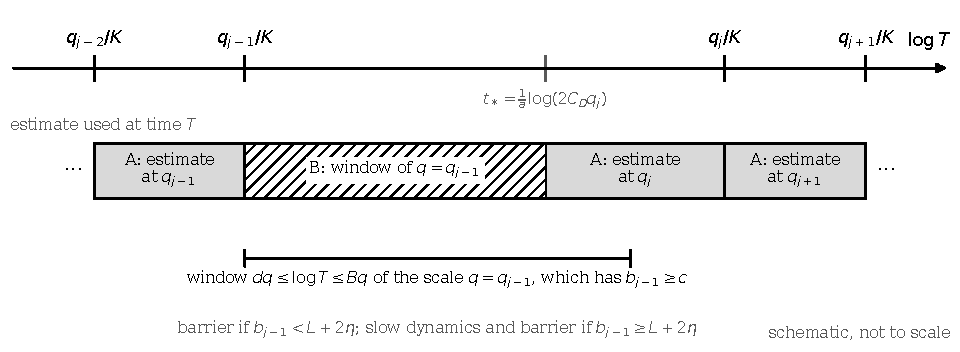
\includegraphics[width=\textwidth]{fig_covering.pdf}
\caption{Schematic of the time covering in the proof of Lemma~\ref{lem:covering}; not to scale, and the positions of the denominators are arbitrary. Here $\beta(\alpha)<\infty$ and $\theta\in G_\alpha^*$ is fixed. Fix $a\in(\max\{0,1-L/\beta(\alpha)\},1)$ and $m>0$, choose $K\ge1$ with $\kappa K>m+3$, and for a large time $T$ let $q_j$ be the first denominator with $q_j\ge K\log T$, so that $\log T\in(q_{j-1}/K,q_j/K]$. If $q_j\le T^a/(2C_D)$, that is, if $\log T\ge t_*$ (case~A, shaded), Proposition~\ref{prop:dt} at the scale $q_j$ gives $P(T^a,T)=O(T^{-m})$. Otherwise (case~B, hatched), which can happen only after a jump from $q_{j-1}$ to a denominator $q_j>e^{aq_{j-1}/K}/(2C_D)$, the scale $q=q_{j-1}$ has $b_{j-1}\ge c=a/(2K)$ and $\log T/q\in[d,B]$, where $d=1/K$, $B_0>\beta(\alpha)$ is chosen with $\max\{0,1-L/B_0\}<a$, and $B=\max\{2B_0/a,2d\}$. Proposition~\ref{prop:selected} then applies, through the barrier of Proposition~\ref{prop:local} or through Theorem~\ref{thm:window}, according as $b_{j-1}$ is below or at least $L+2\eta$, for the small $\eta>0$ fixed in its proof. Every sufficiently large time falls in one of the two cases, whatever the ratios $b_n$ at other scales; no regularity of these ratios and no overlap of windows at consecutive denominators is assumed.}
\label{fig:covering}
\end{figure}

\begin{theorem}\label{thm:upper}
Let $\lambda>1$, let $\alpha$ be irrational with $\beta(\alpha)<\infty$, and let $\theta\in\Ga^*$. For every $a>\max\{0,1-L/\beta(\alpha)\}$ and every $m>0$, $P(T^a,T)=O(T^{-m})$. Consequently
\[
\au(H_{\lambda,\alpha,\theta})\le\max\Bigl\{0,\ 1-\frac{\log\lambda}{\beta(\alpha)}\Bigr\}.
\]
\end{theorem}

\begin{proof}
For $a<1$ this is Lemma~\ref{lem:covering}. For $a\ge1$ choose $a'\in(\max\{0,1-L/\beta\},1)$ and use $P(T^a,T)\le P(T^{a'},T)$. The bound on $\au$ follows from Lemma~\ref{lem:moments}(3), letting $a$ decrease to $\max\{0,1-L/\beta\}$.
\end{proof}

\section{A lower bound for Lipschitz potentials}\label{sec:lower}

This section proves a lower bound for the fastest exponent $\au$, for every phase, under the arithmetic and Lyapunov-continuity hypotheses of Theorem~\ref{thm:L}. The sampling function may be any Lipschitz function satisfying those hypotheses. For the almost Mathieu operator, Section~\ref{sec:moments} strengthens the lower bound to every positive moment. In this section only, let $v:\T\to\R$ be Lipschitz, let $H_\theta u(n)=u(n+1)+u(n-1)+v(\theta+n\alpha)u(n)$, and let $T(E,x)$, $A_r(E,x)$, $L(E)$ and $\Sigma$ be defined as in Section~\ref{sec:prelim} with this $v$.

\begin{theorem}\label{thm:L}
Let $\alpha$ be irrational with $0<\beta(\alpha)<\infty$. Assume that $L(\cdot)$ is continuous on a neighborhood of a point $E_*\in\Sigma$ with $L(E_*)=\ell:=\min_\Sigma L$. Then for every phase $\theta$,
\[
\au(H_\theta)\ge\max\Bigl\{0,\ 1-\frac{\ell}{\beta(\alpha)}\Bigr\}.
\]
\end{theorem}

For the almost Mathieu operator with $\lambda>1$, $L(E)$ is continuous in $E$ and equals $\log\lambda$ on $\Sigma$~\cite[Theorem~1 and Corollary~2]{BourgainJitomirskaya2002}, so $\ell=\log\lambda$ and, for $0<\beta(\alpha)<\infty$, Theorem~\ref{thm:L} gives $\au\ge\max\{0,1-\log\lambda/\beta(\alpha)\}$ at every phase.

\subsection{Elliptic blocks}

Let $e_1=(1,0)^{\mathsf T}$ and $e_2=(0,1)^{\mathsf T}$. A real determinant-one matrix is elliptic when its trace has modulus less than $2$; it is then conjugate over $\R$ to a rotation. We call the coordinates after this conjugation the rotation frame. The direction of a nonzero vector in that frame is its polarization.

For a finite sequence of energies $E-v_r$, $0\le r<q$, let $T_r=\begin{pmatrix}E-v_r&-1\\1&0\end{pmatrix}$, $C_0=I$, $C_r=T_{r-1}\cdots T_0$ and $\mathcal A=C_q$. Suppose $\mathcal A$ is real and elliptic, $|\tr\mathcal A|<2$. Choose $B\in SL(2,\R)$ with $B^{-1}\mathcal AB=R_\varrho$, the rotation by angle $\varrho$, and put $u_r=e_1^{\mathsf T}C_rB$, the first row of $C_rB$, and
\[
S_{\mathcal A}=\sum_{r=0}^{q-1}\|u_r\|^2,\qquad N_\kappa=\begin{pmatrix}0&0\\-1&0\end{pmatrix},\qquad J_0=\begin{pmatrix}0&-1\\1&0\end{pmatrix}.
\]

\begin{lemma}\label{lem:blocks}
\begin{enumerate}
\item $S_{\mathcal A}=|\partial_E\tr\mathcal A|/|\sin\varrho|$.
\item For every $z\in\C$ and $0\le r\le q$, with $\mathcal A(E+z)$ and $C_r(E+z)$ the products at the energy $E+z$,
\[
\|B^{-1}\mathcal A(E+z)B\|\le e^{|z|S_{\mathcal A}},\qquad\|C_r(E+z)B\|\le\|C_r(E)B\|\,e^{|z|S_{\mathcal A}}.
\]
\item If $|\tr\mathcal A|\le3/2$ and the entries $v_r$ depend on a parameter $\phi$ with $|\partial_\phi v_r|\le\mathrm{Lip}$, then $\|B^{-1}(\partial_\phi\mathcal A)B\|\le C\,\mathrm{Lip}\,|\partial_E\tr\mathcal A|$ and $\|B^{-1}(\partial_E\mathcal A)B\|\le C|\partial_E\tr\mathcal A|$, with an absolute constant $C$.
\item Let $z_{\mathcal A}$ be the fixed point of $\mathcal A$ in the upper half-plane. Any $B\in SL(2,\R)$ with $B(i)=z_{\mathcal A}$ conjugates $\mathcal A$ to a rotation, and $\|B\|^2=\|B^{-1}\|^2=e^{d(i,z_{\mathcal A})}$, where $d$ is the hyperbolic distance. If $|\tr\mathcal A|\le3/2$, then $e^{d(i,z_{\mathcal A})}\le C\|\mathcal A\|$, and $z_{\mathcal A}$ moves with hyperbolic speed at most $C\|B^{-1}\mathcal A'B\|$ under any parameter derivative $\mathcal A'$.
\end{enumerate}
\end{lemma}

\begin{proof}
The insertion identity is the common source of the derivative and complex-energy estimates in parts~1--3; part~4 controls how the conjugating frame changes.
Put $Q_r=B^{-1}C_r^{-1}N_\kappa C_rB$. Since $T_r(E+z)=T_r(E)(I+zN_\kappa)$, telescoping gives
\[
B^{-1}\mathcal A(E+z)B=R_\varrho\prod_{r=q-1}^{0}(I+zQ_r),
\]
with the factors ordered from $r=q-1$ on the left to $r=0$ on the right. A direct computation gives $Q_r=-J_0u_r^{\mathsf T}u_r$, a rank-one matrix with $\|Q_r\|=\|u_r\|^2$. Hence $\|B^{-1}\mathcal A(E+z)B\|\le\prod_r(1+|z|\|u_r\|^2)\le e^{|z|S_{\mathcal A}}$, and the same computation truncated at $r$ gives the second inequality in part~2. Differentiating at $z=0$, $B^{-1}(\partial_E\mathcal A)B=R_\varrho\sum_rQ_r$, and the trace of $R_\varrho(-J_0u_r^{\mathsf T}u_r)$ equals $\sin\varrho\,\|u_r\|^2$, because the symmetric part of $R_\varrho J_0$ is $-\sin\varrho\,I$ and the antisymmetric part has zero quadratic form. This proves part~1. A change of $v_r$ at rate $c_r$ gives in the same way $B^{-1}\mathcal A'B=R_\varrho\sum_rc_rQ_r$, so $\|B^{-1}\mathcal A'B\|\le\max_r|c_r|\,S_{\mathcal A}$. When $|\tr\mathcal A|\le3/2$, $|\sin\varrho|\ge\sqrt7/4$, and part~3 follows from part~1. For part~4, recall that every $M\in SL(2,\R)$ satisfies $\|M\|_{\mathrm{HS}}^2=2\cosh d(i,M(i))$; since its singular values are $\sigma$ and $\sigma^{-1}$, this gives $\|M\|^2=e^{d(i,M(i))}$. Apply this to $B$ and $B^{-1}$. If $B(i)=z_{\mathcal A}$, then $B^{-1}\mathcal AB$ fixes $i$ and is a rotation. Conjugating to that rotation and differentiating $\mathcal A(z_{\mathcal A})=z_{\mathcal A}$ shows that the fixed point moves at hyperbolic speed at most $|1-e^{-2i\varrho}|^{-1}\|B^{-1}\mathcal A'B\|$. Finally $\|\mathcal A\|_{\mathrm{HS}}^2=2+4\sinh^2\bigl(d(i,z_{\mathcal A})\bigr)\sin^2\varrho$, which with $|\sin\varrho|\ge\sqrt7/4$ gives $e^{d(i,z_{\mathcal A})}\le C\|\mathcal A\|$.
\end{proof}

\subsection{Proof of Theorem~\ref{thm:L}}

If $\beta(\alpha)\le\ell$ there is nothing to prove, so assume $\ell<\beta(\alpha)$. Fix $h$ with $\ell<h<\beta(\alpha)$.

\emph{Uniform real growth.} By continuity of $L$ near $E_*$ there is a compact neighborhood $U$ of $E_*$ on which $L<h$. The argument of Lemma~\ref{lem:growth} gives $C_h$ with $\|A_r(E,x)\|\le C_he^{hr}$ for $E\in U$, $x\in\T$ and $r\ge0$. By the product rule, with $D_q=Cqe^{hq}$,
\begin{equation}\label{eq:Dq}
|\partial_E\tr A_q(E,x)|\le D_q,\qquad|\partial_x\tr A_q(E,x)|\le\mathrm{Lip}(v)\,D_q\qquad(E\in U),
\end{equation}
the second almost everywhere in $x$.

\emph{A band near $E_*$.} Choose convergents with $\beta_n\to\beta(\alpha)$; write $q=q_n$, $\delta=\delta_n$. Fix a phase $x_0$ and let $H^{\mathrm{per}}$ be the $q$-periodic operator whose potential repeats $v(x_0+k\alpha)$, $0\le k<q$. Its monodromy is $A_q(E,x_0)$, and it differs in norm by at most $\mathrm{Lip}(v)|\delta|$ from the $p/q$-periodic operator at phase $x_0$. The proof of Lemma~\ref{lem:ratspec}, which uses only the Lipschitz bound on $v$, shows that the phase-union spectrum of the $p/q$-periodic operators converges to $\Sigma$ and lies within $\mathrm{Lip}(v)/(2q)$ of each fixed-phase spectrum. So $\sigma(H^{\mathrm{per}})$ has a point converging to $E_*$. Every band of a $q$-periodic operator with hopping one has width at most $2\pi/q$: distributing the Bloch phase over the $q$ bonds makes the Floquet matrices $2/q$-Lipschitz in the Bloch phase. Hence, for large $n$, an entire band of $H^{\mathrm{per}}$ lies in $U$. On that band $\tr A_q(E,x_0)$ is monotone and takes all values in $[-2,2]$, so the set
\[
S_q=\{E\text{ in the band}:|\tr A_q(E,x_0)|\le1\}
\]
is an interval of length at least $2/D_q$.

\emph{Slowly drifting blocks.} The blocks of the actual operator starting at sites $mq$, for $\theta=x_0$, are $A^{(m)}(E)=A_q(E,x_0+mq\alpha)=A_q(E,x_0+m\delta)$, since $q\alpha=p+\delta$. Let
\[
K_q=\Bigl\lfloor\frac{c_0}{D_q|\delta|}\Bigr\rfloor,\qquad N_q=qK_q,\qquad T_q=C_0K_qD_q,
\]
with $c_0$ small and $C_0$ large fixed constants. Since $\log(1/|\delta|)=b_nq$ and $b_n\to\beta(\alpha)>h$, $K_q\to\infty$. For $E\in S_q$ and $0\le m<K_q$, \eqref{eq:Dq} gives $|\tr A^{(m)}(E)-\tr A_q(E,x_0)|\le\mathrm{Lip}(v)D_qK_q|\delta|\le\mathrm{Lip}(v)c_0\le1/2$, so every block satisfies $|\tr A^{(m)}|\le3/2$.

By Lemma~\ref{lem:blocks}(3)--(4), the fixed points $z_m$ of the blocks $A^{(m)}$ move a total hyperbolic distance $\sum_md(z_m,z_{m+1})\le C\,\mathrm{Lip}(v)D_qK_q|\delta|\le C$. Choose any $B_m\in SL(2,\R)$ with $B_m(i)=z_m$. Since $B_{m+1}^{-1}B_m$ maps $i$ to a point at distance $d(z_m,z_{m+1})$ from $i$, Lemma~\ref{lem:blocks}(4) gives $\|B_{m+1}^{-1}B_m\|=e^{d(z_m,z_{m+1})/2}$, so $\prod_m\|B_{m+1}^{-1}B_m\|\le e^{C}$. By Lemma~\ref{lem:blocks}(1)--(2), each block at the energy $E+i/T_q$ satisfies $\|B_m^{-1}A^{(m)}(E+i/T_q)B_m\|\le e^{CD_q/T_q}$, and the product of $K_q$ such factors is at most $e^{CK_qD_q/T_q}\le e^{C/C_0}$. The endpoint lifts cost at most $Ce^{hq}$ by Lemma~\ref{lem:blocks}(4). A partial last block is handled by the second inequality in Lemma~\ref{lem:blocks}(2). Hence, writing $\Phi(x,z)$ for the transfer matrix of $H_{x_0}$ from site $0$ to site $x$,
\begin{equation}\label{eq:L7}
\max_{0\le x\le N_q}\|\Phi(x,E+i/T_q)\|\le Ce^{2hq}\qquad(E\in S_q).
\end{equation}

\emph{Resolvent.} Let $G(n;z)=\langle\delta_n,(H_{x_0}-z)^{-1}\delta_0\rangle$. For $n\ge1$ the vector $(G(n+1;z),G(n;z))$ is obtained from $(G(1;z),G(0;z))$ by the transfer matrices starting at site $1$, which are bounded as in~\eqref{eq:L7} after a shift of the starting site that changes only constants. Since these matrices have determinant one and $|G(0;E+i/T)|\ge\operatorname{Im}G(0;E+i/T)\ge c/T$ for bounded $E$,
\[
|G(n;E+i/T_q)|^2+|G(n+1;E+i/T_q)|^2\ge cT_q^{-2}e^{-4hq}\qquad(E\in S_q,\ 0\le n\le N_q).
\]
By Parseval's formula, $a(n,T)=(\pi T)^{-1}\int_\R|G(n;E+i/T)|^2\,dE$. Summing over the pairs of sites between $N_q/2$ and $N_q$ gives
\begin{equation}\label{eq:L8}
P(N_q/2,T_q)\ge c\,N_q\,|S_q|\,T_q^{-3}e^{-4hq}\ge T_q^{-C_*}
\end{equation}
for a finite constant $C_*$ depending only on $h$ and $\beta(\alpha)$, because $\log T_q=b_nq+O(\log q)$ and $|S_q|\ge2/D_q$.

\emph{The exponent.} From $\log N_q=(b_n-h)q+O(\log q)$ and $\log T_q=b_nq+O(\log q)$ we get $\log N_q/\log T_q\to1-h/\beta(\alpha)$. By~\eqref{eq:L8}, $M_p(T_q)\ge(N_q/2)^pP(N_q/2,T_q)\ge c(N_q/2)^pT_q^{-C_*}$, so $\beta^+(p)\ge1-h/\beta(\alpha)-C_*/p$. Letting $p\to\infty$ and then $h\downarrow\ell$ proves the theorem for the phase $x_0$. The phase was arbitrary.
\qed

The mass in~\eqref{eq:L8} is only polynomially small, so this argument bounds $\au$ but not each fixed $\beta^+(p)$. The losses are the pointwise bound $|G(0)|\ge c/T$, the two frame changes at the ends of the run, and an energy window of small spectral weight. Section~\ref{sec:moments} removes all three for the almost Mathieu operator.

\section{Every moment and the exact packing dimension}\label{sec:moments}

The lower bound of Section~\ref{sec:lower} gives only a polynomially small Abel-averaged mass near the critical distance. For the almost Mathieu operator, along sufficiently large scales with $b_n\ge c>h>\log\lambda$, this section proves that the mass beyond $Te^{-hq_n}$ tends to one uniformly in phase and in $e^{hq_n}\le T\le|\delta_n|^{-1}$. Two facts drive the proof. First, the rational discriminant is asymptotically arcsine distributed under the single-site spectral measure, so most of that measure lies away from the parabolic band edges (Lemma~\ref{lem:arcsine}). Second, at such energies the square-summable half-line solution of the equation with energy $E+i/T$---the Weyl solution---remains spread over a long run of elliptic blocks (Lemma~\ref{lem:run}). These facts give Theorem~\ref{thm:fraction}, Theorem~\ref{thm:B} and the lower moment bounds. A diagonal resolvent estimate from the same runs gives the lower local-dimension bound; the upper transport bound gives the upper packing-dimension bound. The dependencies are: Lemmas~\ref{lem:arcsine} and~\ref{lem:run} give Theorem~\ref{thm:fraction}, which gives Corollary~\ref{cor:moments} and Theorems~\ref{thm:A} and~\ref{thm:B}; Lemma~\ref{lem:run} gives Lemma~\ref{lem:localmass} and part~1 of Theorem~\ref{thm:C}; Theorem~\ref{thm:A} gives Proposition~\ref{prop:packupper} and part~2 of Theorem~\ref{thm:C}.

Throughout, $\lambda>1$, $v(x)=2\lambda\cos2\pi x$ and $L=\log\lambda$, except in Subsection~\ref{sec:run}, where $v$ is any Lipschitz function. For a phase $\theta$ we write $\mu^\theta$ for the spectral measure of $\delta_0$ for $H_{\lambda,\alpha,\theta}$, and
\[
G(k;z)=\langle\delta_k,(H_{\lambda,\alpha,\theta}-z)^{-1}\delta_0\rangle\qquad(k\in\Z,\ \operatorname{Im}z>0).
\]
Two identities connect these objects with transport. The first is Parseval's formula, already used in Section~\ref{sec:lower}:
\begin{equation}\label{eq:parseval}
a(k,T)=\frac1{\pi T}\int_\R|G(k;E+i/T)|^2\,dE .
\end{equation}
It follows from $(H-E-i/T)^{-1}=i\int_0^\infty e^{-t/T}e^{itE}e^{-itH}\,dt$ and Plancherel's theorem. The second is the spectral theorem: for $z=E+i\eps$ with $\eps>0$,
\begin{equation}\label{eq:poisson}
\sum_{k\in\Z}|G(k;z)|^2=\frac{\operatorname{Im}G(0;z)}{\eps},\qquad
\frac1\pi\operatorname{Im}G(0;z)=\int_\R P_\eps(E-E')\,d\mu^\theta(E'),\qquad P_\eps(x)=\frac{\eps}{\pi(x^2+\eps^2)}.
\end{equation}

\subsection{The arcsine law}

Fix a scale $n$ and write $q=q_n$, $p=p_n$, $\delta=\delta_n$. For the phase $\theta$ put
\[
\Delta_n(E)=P_{q}(E)-2\lambda^{q}\cos(2\pi q\theta),
\]
the discriminant of the periodic operator $H_{\lambda,p/q,\theta}$ (Lemma~\ref{lem:chambers}). For that periodic operator the distribution of $\Delta_n$ under the spectral measure of $\delta_0$ is exactly the arcsine law: by~\eqref{eq:ratmagic}, $\Delta_n(H_{\lambda,p/q,\theta})=S^q+S^{-q}$. The next lemma transfers this to the irrational operator at every scale where $|\delta_n|$ is much smaller than $\lambda^{-q_n}$.

Let $\sigma$ be the arcsine law on $[-2,2]$, with density $1/(\pi\sqrt{4-x^2})$. Its moments are $m_k=\binom{k}{k/2}$ for even $k$ and $m_k=0$ for odd $k$, and $\sigma([-a,a])=\frac2\pi\arcsin(a/2)$ for $0\le a\le2$.

\begin{lemma}[Arcsine law]\label{lem:arcsine}
Let $c>L$ and let $\mathcal N$ be an infinite set of indices with $b_n\ge c$ for $n\in\mathcal N$. For every phase $\theta$ let $\nu_n$ be the image of $\mu^\theta$ under $\Delta_n$. Then $\int x^k\,d\nu_n\to m_k$ for every integer $k\ge0$, uniformly in $\theta$, as $n\to\infty$ in $\mathcal N$. Consequently $\nu_n$ converges weakly to $\sigma$, and for every $0\le\eta<2$,
\[
\lim_{n\in\mathcal N}\mu^\theta\bigl(\{E:|\Delta_n(E)|\le2-\eta\}\bigr)=\frac2\pi\arcsin\Bigl(1-\frac\eta2\Bigr).
\]
\end{lemma}

\begin{proof}
Fix $h\in(L,c)$. By Proposition~\ref{prop:poly}, for large $n$ and every phase,
\[
\Delta_n(H)=Q-V(0)=D+F+R,\qquad D=V-V(0),\quad F=S^q+S^{-q},
\]
where $D$ is diagonal and $R$ has range at most $q$ and norm at most $C_hq^{5/2}e^{hq}|\delta|$. Each of $D$, $F$ and $R$ maps a vector supported in $[-jq,jq]$ to a vector supported in $[-(j+1)q,(j+1)q]$.

Fix $k\ge1$. In the expansion of $\Delta_n(H)^k\delta_0$ the operator $D$ only acts on vectors supported in $[-kq,kq]$, where
\[
|D(i)|=2\lambda^q\bigl|\cos(2\pi(q\theta+i\delta))-\cos(2\pi q\theta)\bigr|\le4\pi\lambda^q\,kq|\delta|.
\]
So $\Delta_n(H)^k\delta_0=(D_k+F+R)^k\delta_0$ with $D_k=D\un_{[-kq,kq]}$. Put $\eps_n=4\pi kq\lambda^q|\delta|+C_hq^{5/2}e^{hq}|\delta|$, so that $\|D_k+R\|\le\eps_n$, and recall $\|F\|\le2$. Expanding the product,
\[
\bigl\|\Delta_n(H)^k\delta_0-F^k\delta_0\bigr\|\le(2+\eps_n)^k-2^k .
\]
Since $b_n\ge c>h>L$, both $q\lambda^q|\delta|=qe^{(L-b_n)q}$ and $q^{5/2}e^{hq}|\delta|=q^{5/2}e^{(h-b_n)q}$ tend to $0$, uniformly in $\theta$, so $\eps_n\to0$. Next, $F^k\delta_0=\sum_i\binom{k}{(k+i)/2}\delta_{iq}$, the sum running over $|i|\le k$ with $i\equiv k\pmod 2$, so $\langle\delta_0,F^k\delta_0\rangle=m_k$. Since $\int x^k\,d\nu_n=\langle\delta_0,\Delta_n(H)^k\delta_0\rangle$, we obtain $|\int x^k\,d\nu_n-m_k|\le(2+\eps_n)^k-2^k\to0$.

The law $\sigma$ has compact support, so it is determined by its moments~\cite[Theorem~30.1]{Billingsley1995}, and convergence of all moments implies $\nu_n\Rightarrow\sigma$~\cite[Theorem~30.2]{Billingsley1995}. Since $\sigma$ has no atoms, weak convergence gives $\nu_n(J)\to\sigma(J)$ for every interval $J$. Take $J=[-2+\eta,2-\eta]$. The convergence is uniform in $\theta$: otherwise there would be $\eps_0>0$, indices $n_k\to\infty$ in $\mathcal N$ and phases $\theta_k$ with $|\nu^{\theta_k}_{n_k}(J)-\sigma(J)|\ge\eps_0$; but the moments of $\nu^{\theta_k}_{n_k}$ still converge to $m_j$ for every $j$, so $\nu^{\theta_k}_{n_k}\Rightarrow\sigma$ and $\nu^{\theta_k}_{n_k}(J)\to\sigma(J)$, a contradiction.
\end{proof}

\begin{lemma}[Uniform arcsine bound]\label{lem:arcsineunif}
Let $c$ and $\mathcal N$ be as in Lemma~\ref{lem:arcsine}, and let $0\le\eta<2$. Then
\[
\liminf_{n\in\mathcal N}\ \inf_{\theta\in\T}\ \mu^\theta\bigl(\{E:|\Delta_n(E)|\le2-\eta\}\bigr)\ge\frac2\pi\arcsin\Bigl(1-\frac\eta2\Bigr).
\]
\end{lemma}

\begin{proof}
Put $a=2-\eta$ and fix $\tau\in(0,a)$. Let $f$ be the continuous function that equals $1$ on $[-a+\tau,a-\tau]$, vanishes outside $(-a,a)$ and is linear on the two remaining intervals, so $0\le f\le\un_{[-a,a]}$. By the Weierstrass theorem there is a polynomial $p_0$ with $|p_0-f|\le\tau$ on $[-3,3]$. Let $d$ be its degree and $A$ a constant with $|p_0(x)|\le A(|x|/3)^d$ for $|x|\ge3$. For an integer $K$ with $2K\ge d$ put
\[
p(x)=p_0(x)-\tau-A(x/3)^{2K}.
\]
Then $p\le\un_{[-a,a]}$ on $\R$: on $[-3,3]$ we have $p\le p_0-\tau\le f\le\un_{[-a,a]}$, and for $|x|\ge3$ we have $p(x)\le|p_0(x)|-A(|x|/3)^{2K}\le0$. Hence, with $\nu_n=\nu_n^\theta$ the image of $\mu^\theta$ under $\Delta_n$,
\[
\mu^\theta\bigl(\{|\Delta_n|\le a\}\bigr)=\int\un_{[-a,a]}\,d\nu_n\ge\int p\,d\nu_n .
\]
The right side is a fixed finite combination of the moments $\int x^k\,d\nu_n$, which converge to $m_k$ uniformly in $\theta$ by the proof of Lemma~\ref{lem:arcsine}. So $\liminf_n\inf_\theta\mu^\theta(\{|\Delta_n|\le a\})\ge\int p\,d\sigma\ge\int f\,d\sigma-2\tau-A(2/3)^{2K}\ge\sigma([-a+\tau,a-\tau])-2\tau-A(2/3)^{2K}$, since $\sigma$ lives on $[-2,2]$. Let $K\to\infty$ ($A$ does not depend on $K$), then $\tau\to0$, and use $\sigma([-a,a])=\frac2\pi\arcsin(a/2)$.
\end{proof}


The proof uses no condition on the phase. The only arithmetic input is $b_n\ge c>L$, which makes the residual $\eps_n$ small on the sites that $k$ steps from the origin can reach.

\subsection{One elliptic run}\label{sec:run}

In this subsection $v:\T\to\R$ is Lipschitz with constant $\mathrm{Lip}(v)$, and $T(E,x)$ and $A_r(E,x)$ are defined with this $v$ as in Section~\ref{sec:lower}. Fix a phase $\theta$ and a convergent $p/q$ of $\alpha$, and put $\delta=q\alpha-p$, so that $x+q\alpha=x+\delta$ in $\T$. Let $z=E+i\eps$ with $E\in\R$ and $\eps>0$, and let $g\in\ell^2(\Z_{\ge0})$ satisfy
\begin{equation}\label{eq:halfline}
g(k+1)+g(k-1)+v(\theta+k\alpha)\,g(k)=z\,g(k)\qquad(k\ge1).
\end{equation}
Cut the half-line into blocks of $q$ sites. Put $x_m=\theta+(mq+1)\alpha$, $\Psi_m=(g(mq+1),g(mq))^{\mathsf T}$ and
\[
\mathcal M_m=\sum_{r=0}^{q-1}|g(mq+1+r)|^2 .
\]
Then $(g(mq+1+r),g(mq+r))^{\mathsf T}=A_r(z,x_m)\Psi_m$ for $0\le r\le q$, and in particular $\Psi_{m+1}=A_q(z,x_m)\Psi_m$. Consecutive blocks see almost the same potential: $x_{m+1}=x_m+\delta$, so the potentials at corresponding sites differ by at most $\mathrm{Lip}(v)|\delta|$. We use the notation $T_r$, $C_r$, $N_\kappa$, $J_0$ and $R_\varrho$ of Lemma~\ref{lem:blocks}, and $d$ for the hyperbolic distance in the upper half-plane, normalized as there.

The first lemma is the telescoping identity behind Lemma~\ref{lem:blocks}, for site-dependent shifts.

\begin{lemma}[Insertion]\label{lem:insert}
Let $T_r$ and $C_r$ be as in Lemma~\ref{lem:blocks} for energies $E-v_r$, $0\le r<q$, let $B\in SL(2,\R)$, and put $u_r=e_1^{\mathsf T}C_rB$. Let $w_0,\dots,w_{q-1}\in\C$ and let $C_r'$ be the products for the energies $E-v_r+w_r$. Then for $0\le r\le q$,
\[
C_r'B=C_rB\,\Pi_r,\qquad\Pi_r=(I+w_{r-1}Q_{r-1})\cdots(I+w_0Q_0),\qquad Q_j=-J_0u_j^{\mathsf T}u_j,
\]
with $\det\Pi_r=1$ and $\|\Pi_r-I\|\le\exp\bigl(\sum_{j<r}|w_j|\,\|u_j\|^2\bigr)-1$.
\end{lemma}

\begin{proof}
The new one-step matrices are $T_j(I+w_jN_\kappa)$. If $C_j'B=C_jB\Pi_j$, then
\[
C_{j+1}'B=T_j(I+w_jN_\kappa)C_jB\Pi_j=C_{j+1}B\,(I+w_jB^{-1}C_j^{-1}N_\kappa C_jB)\,\Pi_j ,
\]
which gives the product formula by induction. The computation in the proof of Lemma~\ref{lem:blocks}, which uses only $\det B=\det C_j=1$, gives $B^{-1}C_j^{-1}N_\kappa C_jB=-J_0u_j^{\mathsf T}u_j$. This matrix has norm $\|u_j\|^2$, and it has trace $-u_jJ_0u_j^{\mathsf T}=0$ and rank one, so $\det(I+w_jQ_j)=1$. Expanding the product gives the norm bound.
\end{proof}

\begin{lemma}[Perturbed rotations]\label{lem:rot}
Let $|\sin\varrho|\ge s>0$ and let $M=R_\varrho(I+Y)\in SL(2,\R)$ with $\|Y\|\le y\le s/8$. Then $M$ is elliptic, and its fixed point $w$ in the upper half-plane satisfies $d(i,w)\le12y/s$.
\end{lemma}

\begin{proof}
The unitary matrix $\mathcal C=2^{-1/2}\begin{pmatrix}1&-i\\1&i\end{pmatrix}$ acts as the Cayley map from the upper half-plane to the unit disc, sends $i$ to $0$, and is an isometry for the hyperbolic metrics. It conjugates $R_\varrho$ to $\mathrm{diag}(e^{-i\varrho},e^{i\varrho})$ and $M$ to a matrix $\begin{pmatrix}a&b\\\bar b&\bar a\end{pmatrix}$ with $|a|^2-|b|^2=1$. Since $\mathcal C$ is unitary, $\|\mathcal CM\mathcal C^{-1}-\mathcal CR_\varrho\mathcal C^{-1}\|=\|R_\varrho Y\|\le y$, so $|b|\le y$ and $|\operatorname{Im}a|\ge s-y\ge\frac78s>|b|$. Hence $M$ is elliptic. The fixed point of $\zeta\mapsto(a\zeta+b)/(\bar b\zeta+\bar a)$ in the disc solves $\bar b\zeta^2-2i(\operatorname{Im}a)\zeta-b=0$ and has modulus
\[
t=\frac{|b|}{|\operatorname{Im}a|+\sqrt{(\operatorname{Im}a)^2-|b|^2}}\le\frac{8y}{7s}\le\frac14 .
\]
Its hyperbolic distance from $0$ is $\log\frac{1+t}{1-t}\le\frac{2t}{1-t}\le\frac83t\le12y/s$.
\end{proof}

\begin{lemma}[Pair inequality]\label{lem:pair}
Let $G$ be a real symmetric positive semidefinite $2\times2$ matrix with trace $S$, and let $R_\varrho$ be a rotation. Then $\Phi^*(G+R_\varrho^{\mathsf T}GR_\varrho)\Phi\ge S(1-|\cos\varrho|)\|\Phi\|^2$ for every $\Phi\in\C^2$.
\end{lemma}

\begin{proof}
Write $G=\frac S2I+gF_\phi$ with $F_\phi=\begin{pmatrix}\cos\phi&\sin\phi\\\sin\phi&-\cos\phi\end{pmatrix}$ and $0\le g\le S/2$. Since $R_\varrho^{\mathsf T}F_\phi R_\varrho=F_{\phi-2\varrho}$ and $F_\phi+F_{\phi-2\varrho}=2\cos\varrho\,F_{\phi-\varrho}$, the real symmetric matrix $G+R_\varrho^{\mathsf T}GR_\varrho=SI+2g\cos\varrho\,F_{\phi-\varrho}$ has eigenvalues $S\pm2g|\cos\varrho|\ge S(1-|\cos\varrho|)$. A real symmetric matrix bounds its Hermitian form on $\C^2$ below by its smallest eigenvalue.
\end{proof}

The point of Lemma~\ref{lem:pair} is that it holds for every polarization $\Phi$. A single block may carry little mass, for instance when the solution is a standing wave with a node there, but two adjacent blocks cannot both do so.

\begin{lemma}[Elliptic propagation]\label{lem:run}
Let $0<\eta\le1$ and assume $|\tr A_q(E,x_0)|\le2-\eta$. Let $B_0\in SL(2,\R)$ map $i$ to the fixed point of $A_q(E,x_0)$ in the upper half-plane, and put
\[
S_0=\sum_{r=0}^{q-1}\|e_1^{\mathsf T}A_r(E,x_0)B_0\|^2,\qquad\Phi_0=B_0^{-1}\Psi_0,
\]
\[
\xi=(\mathrm{Lip}(v)+1)\max(\eps,|\delta|),\qquad m_*=\Bigl\lfloor\frac{\eta^{3/2}}{2^{10}\xi S_0}\Bigr\rfloor .
\]
If $m_*\ge8$, then:
\begin{enumerate}
\item for $0\le m<m_*$, $\ \mathcal M_m+\mathcal M_{m+1}\ge2^{-8}\eta\,S_0\|\Phi_0\|^2$ and $\mathcal M_m\le16S_0\|\Phi_0\|^2$;
\item with $m_0=\lceil m_*/2\rceil$,
\[
\sum_{k>m_0q}|g(k)|^2\ge\frac{\eta^{5/2}}{2^{22}}\cdot\frac{\|\Phi_0\|^2}{\xi};
\]
\item $\sum_{k>m_*q}|g(k)|^2\le2\|\Phi_0\|^2/\eps$, $\ \sum_{k\ge1}|g(k)|^2\le(1/\xi+2/\eps)\|\Phi_0\|^2$, and $|g(0)|\le\|B_0\|\,\|\Phi_0\|$.
\end{enumerate}
\end{lemma}

By Lemma~\ref{lem:blocks}(1), $S_0=|\partial_E\tr A_q(E,x_0)|/|\sin\varrho_0|$, where $\varrho_0$ is the rotation angle of $A_q(E,x_0)$. For fixed $\eta$, the run consists of $m_*$ blocks and has length comparable to $q/(\xi S_0)$, with comparison constants depending on $\eta$. Its length is set by the larger of the damping $\eps$ and the drift $|\delta|$; it is not a fixed function of the scale. When $\eps\ge|\delta|$, the total mass in part~3 is at most $3(\mathrm{Lip}(v)+1)\|\Phi_0\|^2/\xi$, so part~2 says that the far half of the run carries a fixed fraction of the mass of $g$ on $\Z_{>0}$. No arithmetic condition on $\theta$ enters, and nothing is assumed about the solution beyond the run.

\begin{proof}
\emph{Frames.} Write $A_m=A_q(E,x_m)$ for the real-energy block monodromies. Suppose $A_m$ is elliptic and $B_m\in SL(2,\R)$ maps $i$ to its fixed point, so that $B_m^{-1}A_mB_m=R_{\varrho_m}$ by Lemma~\ref{lem:blocks}(4). Put
\[
u_r^{(m)}=e_1^{\mathsf T}A_r(E,x_m)B_m,\qquad G_m=\sum_{r=0}^{q-1}(u_r^{(m)})^{\mathsf T}u_r^{(m)},\qquad S_m=\tr G_m,\qquad\Phi_m=B_m^{-1}\Psi_m .
\]

\emph{One step.} Apply Lemma~\ref{lem:insert} with $B=B_m$ and the shifts $w_r=v(x_m+r\alpha)-v(x_{m+1}+r\alpha)$, which satisfy $|w_r|\le\mathrm{Lip}(v)|\delta|$. It gives, for $0\le r\le q$,
\[
A_r(E,x_{m+1})B_m=A_r(E,x_m)B_m\,\Pi^{(m)}_r,\qquad\|\Pi^{(m)}_r-I\|\le y_m:=e^{\mathrm{Lip}(v)|\delta|S_m}-1 .
\]
In particular $B_m^{-1}A_{m+1}B_m=R_{\varrho_m}\Pi^{(m)}_q$ and $|\tr A_{m+1}-\tr A_m|\le2y_m$. Put $s_0=\sqrt\eta/2$. If $|\sin\varrho_m|\ge s_0$ and $y_m\le s_0/8$, Lemma~\ref{lem:rot} shows that $A_{m+1}$ is elliptic with fixed point $B_m(w_m)$, where $d(i,w_m)\le d_m:=12y_m/s_0$. Choose $N_m\in SL(2,\R)$ with $N_m(i)=w_m$; by Lemma~\ref{lem:blocks}(4), $\|N_m\|^2=\|N_m^{-1}\|^2=e^{d(i,w_m)}\le e^{d_m}$. Then $B_{m+1}=B_mN_m$ maps $i$ to the fixed point of $A_{m+1}$.

\emph{The damped step.} Lemma~\ref{lem:insert} with $B=B_m$ and the constant shift $w_r=i\eps$ gives $A_q(z,x_m)B_m=B_mR_{\varrho_m}\Pi'_m$ with $\det\Pi'_m=1$ and $\|\Pi'_m-I\|\le e^{\eps S_m}-1$. Hence
\[
\Phi_{m+1}=N_m^{-1}R_{\varrho_m}\Pi'_m\,\Phi_m .
\]

\emph{Bootstrap.} We show by induction that for $0\le m\le m_*$ the frame $B_m$ is defined and
\[
(a_m)\qquad|\tr A_m|\le2-\eta/2,\qquad S_0/2\le S_m\le2S_0,\qquad\|\Phi_0\|/2\le\|\Phi_m\|\le2\|\Phi_0\|.
\]
$(a_0)$ holds. Assume $(a_j)$ for all $j<m$, where $m\le m_*$. Note that $\eps\le\xi$ and $\mathrm{Lip}(v)|\delta|\le\xi$, and that $m_*\ge1$ forces $\xi S_0\le2^{-10}\eta^{3/2}$. For $j<m$ we have $|\cos\varrho_j|\le1-\eta/4$, hence $\sin^2\varrho_j\ge\eta/4$ and $|\sin\varrho_j|\ge s_0$. Also $\mathrm{Lip}(v)|\delta|S_j\le2\xi S_0\le1$, and $e^x-1\le2x$ for $0\le x\le1$, so
\[
y_j\le4\xi S_0\le2^{-8}\eta^{3/2}\le s_0/8 .
\]
So the frames $B_1,\dots,B_m$ are defined. Summing the one-step estimates over $j<m$:
\begin{itemize}
\item $|\tr A_m-\tr A_0|\le2\sum_{j<m}y_j\le8m_*\xi S_0\le2^{-7}\eta^{3/2}\le\eta/2$, so $|\tr A_m|\le2-\eta/2$.
\item $u_r^{(j+1)}=u_r^{(j)}\Pi^{(j)}_rN_j$, so, since $\|u\Pi^{(j)}_r\|\ge\|u\|-\|u(\Pi^{(j)}_r-I)\|$ and $\|uN_j\|\ge\|u\|/\|N_j^{-1}\|$, $S_{j+1}/S_j\in[(1-y_j)^2e^{-d_j},(1+y_j)^2e^{d_j}]$ and $|\log(S_{j+1}/S_j)|\le3y_j+d_j\le27y_j/\sqrt\eta$. Hence $|\log(S_m/S_0)|\le108\,m_*\xi S_0/\sqrt\eta\le108\eta/2^{10}<\log2$.
\item A $2\times2$ matrix of determinant one has $\|M^{-1}\|=\|M\|$, and $\|\Pi'_j\|\le e^{\eps S_j}$. So $|\log(\|\Phi_{j+1}\|/\|\Phi_j\|)|\le\eps S_j+d_j/2\le2\xi S_0+12y_j/\sqrt\eta\le50\xi S_0/\sqrt\eta$, and $|\log(\|\Phi_m\|/\|\Phi_0\|)|\le50\eta/2^{10}<\log2$.
\end{itemize}
This proves $(a_m)$.

\emph{Pairs of blocks.} Fix $0\le m<m_*$ and put $\eps_2=e^{3\xi S_m}-1$. Since $3\xi S_m\le6\xi S_0\le1$, we have $\eps_2\le12\xi S_0\le12\cdot2^{-10}\eta^{3/2}$. By Lemma~\ref{lem:insert} with the shift $i\eps$,
\[
g(mq+1+r)=e_1^{\mathsf T}A_r(z,x_m)B_m\Phi_m=u_r^{(m)}(\Phi_m+e_r),\qquad\|e_r\|\le\eps_2\|\Phi_m\| .
\]
For the next block, $\Psi_{m+1}=B_mR_{\varrho_m}\Pi'_m\Phi_m$. Apply Lemma~\ref{lem:insert} first with the phase shifts, which gives $A_r(E,x_{m+1})B_m=A_r(E,x_m)B_m\Pi^{(m)}_r$, and then with the shift $i\eps$, for which the rows $u_r^{(m)}\Pi^{(m)}_r$ have squared norms at most $(1+y_m)^2\|u_r^{(m)}\|^2\le2\|u_r^{(m)}\|^2$. This gives
\[
g((m+1)q+1+r)=u_r^{(m)}\,\Pi^{(m)}_r\Pi''_r\,R_{\varrho_m}\Pi'_m\,\Phi_m=u_r^{(m)}(R_{\varrho_m}\Phi_m+e_r'),
\]
where $\|\Pi''_r-I\|\le e^{2\eps S_m}-1$. The three factors $\Pi^{(m)}_r$, $\Pi''_r$ and $\Pi'_m$ differ from $I$ by at most $e^{\mathrm{Lip}(v)|\delta|S_m}-1$, $e^{2\eps S_m}-1$ and $e^{\eps S_m}-1$, and $R_{\varrho_m}$ is orthogonal. Hence $\|\Pi^{(m)}_r\Pi''_rR_{\varrho_m}\Pi'_m-R_{\varrho_m}\|\le e^{(\mathrm{Lip}(v)|\delta|+3\eps)S_m}-1\le\eps_2$, because $\mathrm{Lip}(v)|\delta|+3\eps\le3\xi$. So $\|e_r'\|\le\eps_2\|\Phi_m\|$.

For every $e\in\C^2$, $\sum_r|u_r^{(m)}e|^2=e^*G_me\le S_m\|e\|^2$, and $\Phi^*G_m\Phi=\sum_r|u_r^{(m)}\Phi|^2$. Apply $\|a+b\|^2\ge\frac12\|a\|^2-\|b\|^2$ to vectors indexed by $0\le r<q$:
\[
\mathcal M_m\ge\tfrac12\Phi_m^*G_m\Phi_m-S_m\eps_2^2\|\Phi_m\|^2,\qquad
\mathcal M_{m+1}\ge\tfrac12\Phi_m^*R_{\varrho_m}^{\mathsf T}G_mR_{\varrho_m}\Phi_m-S_m\eps_2^2\|\Phi_m\|^2 .
\]
By $(a_m)$, $|\cos\varrho_m|\le1-\eta/4$, so Lemma~\ref{lem:pair} and $2\eps_2^2\le\eta/16$ give
\[
\mathcal M_m+\mathcal M_{m+1}\ge\Bigl(\frac\eta8-2\eps_2^2\Bigr)S_m\|\Phi_m\|^2\ge\frac\eta{16}S_m\|\Phi_m\|^2\ge\frac{\eta}{2^7}S_0\|\Phi_0\|^2 .
\]
Also $\mathcal M_m\le(1+\eps_2)^2S_m\|\Phi_m\|^2\le16S_0\|\Phi_0\|^2$. This proves part~1.

\emph{Flux.} Multiply~\eqref{eq:halfline} by $\overline{g(k)}$, sum over $k>n$ for some $n\ge0$, and take imaginary parts. Since $g\in\ell^2$ and $\sum_{k>n}2\operatorname{Re}\bigl(g(k+1)\overline{g(k)}\bigr)$ is real,
\[
\eps\sum_{k>n}|g(k)|^2=\operatorname{Im}\bigl(g(n)\overline{g(n+1)}\bigr).
\]
If $(g(n+1),g(n))^{\mathsf T}=B\Phi$ with $B$ real and $\det B=1$, then $2|\operatorname{Im}(g(n)\overline{g(n+1)})|=|\det(B\Phi,B\bar\Phi)|=|\det(\Phi,\bar\Phi)|\le\|\Phi\|^2$. At $n=m_*q$ this gives $\sum_{k>m_*q}|g(k)|^2\le\|\Phi_{m_*}\|^2/(2\eps)\le2\|\Phi_0\|^2/\eps$.

\emph{Counting.} Let $X=\eta^{3/2}/(2^{10}\xi S_0)$, so that $X\ge m_*\ge8$ and $m_*\ge X/2$. The blocks $m_0,\dots,m_*$ lie in $\{k>m_0q\}$ and contain at least $\lfloor m_*/2\rfloor/2\ge m_*/8$ disjoint pairs $(m,m+1)$ with $m<m_*$. By part~1,
\[
\sum_{k>m_0q}|g(k)|^2\ge\frac{m_*}8\cdot\frac{\eta}{2^8}S_0\|\Phi_0\|^2\ge\frac{X}{16}\cdot\frac{\eta}{2^8}S_0\|\Phi_0\|^2=\frac{\eta^{5/2}}{2^{22}}\cdot\frac{\|\Phi_0\|^2}{\xi}.
\]
For part~3, $\sum_{k\ge1}|g(k)|^2=\sum_{m<m_*}\mathcal M_m+\sum_{k>m_*q}|g(k)|^2$, and $16m_*S_0\le16XS_0=2^{-6}\eta^{3/2}/\xi\le1/\xi$. Finally $g(0)=e_2^{\mathsf T}\Psi_0=e_2^{\mathsf T}B_0\Phi_0$.
\end{proof}

\subsection{Almost all of the packet at resonant times}

From now on $v(x)=2\lambda\cos2\pi x$ again, so $\mathrm{Lip}(v)=4\pi\lambda$. We first compare the traces of the actual $q$-blocks with the rational discriminant.

\begin{lemma}[Block traces]\label{lem:blocktrace}
For every $h>L$ there is $C$ such that for all large $n$, all real $E\in U_h$ and all $x\in\T$,
\[
\bigl|\tr A_{q_n}(E,x)-P_{q_n}(E)+2\lambda^{q_n}\cos(2\pi q_nx)\bigr|\le C\,q_ne^{hq_n}|\delta_n| .
\]
\end{lemma}

\begin{proof}
By Lemma~\ref{lem:chambers}, $P_q(E)-2\lambda^q\cos(2\pi qx)=\tr A^{(p/q)}_q(E,x)$. As in Step~1 of the proof of Proposition~\ref{prop:poly}, write each rational factor as the irrational one plus an error of norm at most $d=4\pi\lambda|\delta|$ and expand. The difference $A^{(p/q)}_q(E,x)-A_q(E,x)$ is the sum of the terms with at least one error, so its norm is at most
\[
\sum_{k=1}^q\binom qkC_h^{k+1}e^{h(q-k)}d^k=C_he^{hq}\bigl[(1+C_hde^{-h})^q-1\bigr]\le C_h^2qd\,e^{hq}e^{C_hqd},
\]
and $qd\le4\pi\lambda$. The trace of a $2\times2$ matrix is at most twice its norm.
\end{proof}

\begin{theorem}[Almost all of the packet moves out]\label{thm:fraction}
Let $\lambda>1$, let $\alpha$ be irrational and let $\theta$ be any phase. Fix $h>L$, $c>h$ and $0<\eta\le1/4$. There are $C$ and $n_0$, depending only on $\lambda$, $\alpha$, $h$, $c$ and $\eta$, such that for every $n\ge n_0$ with $b_n\ge c$ and every $T$ with $e^{hq_n}\le T\le|\delta_n|^{-1}$,
\[
P\bigl(Te^{-hq_n},T\bigr)\ge\bigl(1-Cq_ne^{-(h-L)q_n/2}\bigr)\,\mu^\theta\bigl(\{E:|\Delta_n(E)|\le2-3\eta\}\bigr).
\]
\end{theorem}

If $b_n\ge c$ for infinitely many $n$, then along those $n$ the factor $\mu^\theta(\cdot)$ is at least $\frac2\pi\arcsin(1-\frac{3\eta}2)-o(1)$, uniformly in $\theta$, by Lemma~\ref{lem:arcsineunif}; since $\eta$ is arbitrary, the Abel-averaged probability beyond $Te^{-hq_n}$ tends to $1$ (Theorem~\ref{thm:B}). At the resonant time $T=|\delta_n|^{-1}=e^{b_nq_n}$ the distance is $e^{(b_n-h)q_n}=T^{1-h/b_n}$. The mechanism is visible in the proof: at an energy whose first $q$-blocks on both sides are elliptic, the resolvent $G(\cdot;E+i/T)$ has, on each side, comparable mass on every pair of adjacent blocks among at least $c'T/(qe^{h_0q})$ consecutive $q$-blocks, and at most $16S_0\|\Phi_0\|^2$ on each of them (Lemma~\ref{lem:run}(1)); so the at most $Te^{-hq}/q+1$ blocks within distance $Te^{-hq}$ carry only a fraction $O(qe^{-(h-h_0)q})$ of it, with $h_0=(L+h)/2$. The mass beyond the run, which the earlier version of this argument counted against the fraction, is itself beyond $Te^{-hq}$.

\begin{proof}
Let $h_0=(L+h)/2$ and $U=U_{h_0}$. By Lemma~\ref{lem:growth} and Proposition~\ref{prop:poly}(2) there is $C$ with $\|A_r(E,x)\|\le Ce^{h_0r}$ for real $E\in U$, all $x$ and $r\ge0$, and $\sup_U|P_q'|\le Cqe^{h_0q}$. Write $q=q_n$, $\delta=\delta_n$, $b=b_n$ and $\eps=1/T$, so that $|\delta|\le\eps\le e^{-hq}$, and put
\[
N=Te^{-hq},\qquad I=\{E\in U:\ |\Delta_n(E)|\le2-2\eta\}.
\]
Below, $C$ and $c'$ denote positive constants depending only on $\lambda$, $\alpha$, $h$ and $\eta$, and ``for large $n$'' means for $n$ beyond a threshold depending only on $\lambda$, $\alpha$, $h$, $c$ and $\eta$; nothing depends on $\theta$ or $T$. Note that $h_0-h=-(h-L)/2$.

\emph{Step 1: two elliptic first blocks.} Fix $E\in I$ and $z=E+i\eps$. For $k\ge0$ put $g_+(k)=G(k;z)$ and $g_-(k)=G(-k;z)$. Both lie in $\ell^2(\Z_{\ge0})$. The function $g_+$ satisfies~\eqref{eq:halfline} for the phase $\theta$. Since the cosine is even, $v(\theta-k\alpha)=v(-\theta+k\alpha)$, so $g_-$ satisfies~\eqref{eq:halfline} for the phase $-\theta$. The first blocks are $A_q(E,\pm\theta+\alpha)$. Since $q(\pm\theta+\alpha)=\pm q\theta+p+\delta$, Lemma~\ref{lem:blocktrace} and $|\cos(2\pi(\pm q\theta+\delta))-\cos(2\pi q\theta)|\le2\pi|\delta|$ give
\[
\bigl|\tr A_q(E,\pm\theta+\alpha)-\Delta_n(E)\bigr|\le Cqe^{h_0q}|\delta|+4\pi\lambda^q|\delta| .
\]
The right side tends to $0$ because $b\ge c>h_0>L$. So for large $n$ both first blocks satisfy $|\tr A_q|\le2-\eta$.

\emph{Step 2: the run is long and the near blocks are few.} Apply Lemma~\ref{lem:run} to $g_\pm$, with this $\eta$, the damping $\eps$ and $\xi=(4\pi\lambda+1)\eps$ (recall $\eps\ge|\delta|$), and let $B_0^\pm$, $S_0^\pm$, $\Phi_0^\pm$, $m_*^\pm$, $m_0^\pm$ be the corresponding data. From $|\tr A_q|\le2-\eta$ we get $|\sin\varrho_0^\pm|\ge\sqrt\eta/2$, and the product rule gives $|\partial_E\tr A_q(E,x)|\le2qC^2e^{h_0q}$. By Lemma~\ref{lem:blocks}(1), $S_0^\pm\le Cqe^{h_0q}$. Hence
\[
\frac{\eta^{3/2}}{2^{10}\xi S_0^\pm}\ge\frac{c'T}{qe^{h_0q}}\ge\frac{c'e^{(h-h_0)q}}{q},
\]
so for large $n$ we have $m_*^\pm\ge8$, and $m_0^\pm q\ge m_*^\pm q/2\ge c'Te^{-h_0q}/4\ge Te^{-hq}=N$.

\emph{Far mass.} Lemma~\ref{lem:run}(2) and $m_0^\pm q\ge N$ give
\begin{equation}\label{eq:farlower}
\sum_{k>N}|g_\pm(k)|^2\ge\frac{\eta^{5/2}}{2^{22}}\cdot\frac{\|\Phi_0^\pm\|^2}{\xi}.
\end{equation}

\emph{Near mass.} The sites $1\le k\le N$ lie in the blocks $\{mq+1,\dots,mq+q\}$ with $0\le m\le(N-1)/q$, which are at most $N/q+1$ blocks, and $(N-1)/q<m_0^\pm\le m_*^\pm-1$ because $m_*^\pm\ge8$. So Lemma~\ref{lem:run}(1) applies to each of them, and with~\eqref{eq:farlower},
\[
\sum_{k=1}^N|g_\pm(k)|^2\le\Bigl(\frac Nq+1\Bigr)16S_0^\pm\|\Phi_0^\pm\|^2\le2^{26}\eta^{-5/2}\Bigl(\frac Nq+1\Bigr)S_0^\pm\xi\sum_{k>N}|g_\pm(k)|^2 .
\]
Here, using $S_0^\pm\le Cqe^{h_0q}$, $\xi=(4\pi\lambda+1)/T$, $N=Te^{-hq}$ and $T\ge e^{hq}$,
\[
\Bigl(\frac Nq+1\Bigr)S_0^\pm\xi\le C(4\pi\lambda+1)\Bigl(e^{(h_0-h)q}+\frac{qe^{h_0q}}T\Bigr)\le C(4\pi\lambda+1)(1+q)e^{-(h-L)q/2}.
\]

\emph{The site $0$.} By Lemma~\ref{lem:blocks}(4), $\|B_0^+\|^2=e^{d(i,z_+)}$, where $z_+$ is the fixed point of $\mathcal A=A_q(E,\theta+\alpha)$. The identity $\|\mathcal A\|_{\mathrm{HS}}^2=2+4\sinh^2(d(i,z_+))\sin^2\varrho_0^+$ from the proof of Lemma~\ref{lem:blocks}(4) gives $\|B_0^+\|^2\le1+4\|\mathcal A\|/\sqrt\eta\le Ce^{h_0q}$. With part~3 of Lemma~\ref{lem:run} and~\eqref{eq:farlower},
\[
|G(0;z)|^2\le\|B_0^+\|^2\|\Phi_0^+\|^2\le Ce^{h_0q}\xi\sum_{k>N}|g_+(k)|^2\le C(4\pi\lambda+1)e^{-(h-L)q/2}\sum_{k>N}|g_+(k)|^2 .
\]

\emph{Conclusion of Step 2.} Since $g_+(k)=G(k;z)$ and $g_-(k)=G(-k;z)$ for $k\ge1$, adding the last three displays gives, for large $n$,
\[
\sum_{|k|\le N}|G(k;z)|^2\le\kappa_n\sum_{|k|>N}|G(k;z)|^2,\qquad\kappa_n=Cqe^{-(h-L)q/2},
\]
and therefore
\begin{equation}\label{eq:farfraction}
\sum_{|k|>N}|G(k;z)|^2\ge(1-\kappa_n)\sum_{k\in\Z}|G(k;z)|^2\qquad(E\in I).
\end{equation}

\emph{Step 3: Parseval.} By~\eqref{eq:parseval}, \eqref{eq:farfraction} and~\eqref{eq:poisson},
\[
P(N,T)=\frac1{\pi T}\int_\R\sum_{|k|>N}|G(k;E+i\eps)|^2\,dE\ge(1-\kappa_n)\int_I\frac1\pi\operatorname{Im}G(0;E+i\eps)\,dE ,
\]
and the right side equals $(1-\kappa_n)\int_\R\bigl(\int_IP_\eps(E-E')\,dE\bigr)\,d\mu^\theta(E')$.

\emph{Step 4: Poisson smoothing.} Let $r_*>0$ be the distance from $\Sigma$ to $\R\setminus U$, and $r=\min(r_*/2,\eta/\sup_U|P_q'|)$, so that $r\ge\eta/(Cqe^{h_0q})$ for large $n$. If $E'\in\Sigma$ and $|\Delta_n(E')|\le2-3\eta$, then $[E'-r,E'+r]\subset U$, and $\Delta_n'=P_q'$ gives $|\Delta_n|\le2-2\eta$ there. So $[E'-r,E'+r]\subset I$ and
\[
\int_IP_\eps(E-E')\,dE\ge\frac2\pi\arctan\frac r\eps\ge1-\frac{2\eps}{\pi r} .
\]
Since $\eps/r\le Cqe^{h_0q}/(\eta T)\le Cqe^{-(h-L)q/2}$ and $\mu^\theta$ is supported on $\Sigma$, we obtain $P(N,T)\ge(1-\kappa_n)(1-Cqe^{-(h-L)q/2})\,\mu^\theta(\{|\Delta_n|\le2-3\eta\})$, which is the claim after enlarging $C$.
\end{proof}

\begin{remark}[Where the old constant was lost]\label{rem:oldconstant}
An earlier version compared the far mass~\eqref{eq:farlower} with the whole mass $\sum_{k\ge1}|g_\pm(k)|^2\le3(4\pi\lambda+1)\|\Phi_0^\pm\|^2/\xi$ of Lemma~\ref{lem:run}(3), which produced the factor $\eta^{5/2}2^{-24}/(4\pi\lambda+1)$, and then took $\eta=1/4$ and $\mu^\theta(\{|\Delta_n|\le5/4\})\ge1/4$, which gives $2^{-31}/(1+4\pi\lambda)$; an extra factor $1/2$, taken in the eventual Poisson-smoothing bound, produced $2^{-32}/(1+4\pi\lambda)$. The upper bound of Lemma~\ref{lem:run}(3) counts the mass beyond the run, but that mass is also beyond $N$. The flux identity, the Parseval step and the Poisson smoothing lose only factors $1-o(1)$; the only genuine loss is the spectral mass near the band edges, $1-\frac2\pi\arcsin(1-\frac{3\eta}2)\approx\frac2\pi\sqrt{3\eta}$, which disappears as $\eta\to0$.
\end{remark}

\begin{remark}[An annulus at strongly resonant scales]\label{rem:burst}
Theorem~\ref{thm:fraction} has a matching upper half. Let $\theta\in\Ga^*$ and $\beta(\alpha)<\infty$, and fix $B_0>\beta(\alpha)$, $h>L$, $c>h$, $\eps>0$ and $M>0$. Let $\zeta_1$ be given by Theorem~\ref{thm:window} for $\eta=c-L$, this $\eps$ and $M$, and $\Lambda=\max(1,B_0)$. For large $n$ with $b_n\ge c$ we have $b_n\le B_0$ and, since $\theta\in\Ga^*$, $|\sin(2\pi q_n\theta)|\ge e^{-\zeta_1q_n}$; this threshold in $n$ may depend on the fixed phase. For every $T$ with $e^{hq_n}\le T\le|\delta_n|^{-1}$ put
\[
N_-=Te^{-hq_n}=T\lambda^{-q_n}e^{-(h-L)q_n},\qquad N_+=e^{\eps q_n}\bigl(1+T\lambda^{-q_n}\bigr)\le2e^{\eps q_n}T\lambda^{-q_n}.
\]
Theorem~\ref{thm:window}, whose time range contains $T\le|\delta_n|^{-1}\le e^{B_0q_n}$, gives $P(N_+,T)\le Ce^{-Mq_n}$, and Theorem~\ref{thm:B}, which is deduced from Theorem~\ref{thm:fraction} and Lemma~\ref{lem:arcsineunif} in Section~\ref{sec:everymoment}, gives $P(N_-,T)\ge1-o(1)$ as $n\to\infty$ with $b_n\ge c$, uniformly in $T$. So the annulus $N_-<|j|\le N_+$ carries Abel-averaged mass $1-o(1)$: asymptotically the whole Abel-averaged packet lies at distance $T\lambda^{-q_n}$, up to the factors $e^{(h-L)q_n}$ and $2e^{\eps q_n}$, whose exponents can be fixed as small as we like before $n$ is taken large. In particular, for each fixed $s\in(0,1)$, the $s$-quantile of the Abel-averaged distribution $j\mapsto a(j,T)$ of $|j|$ (the median for $s=1/2$) lies in $[N_-,N_+]$ for all large $n$ with $b_n\ge c$, uniformly in $T$. The window begins at $T=e^{hq_n}=\lambda^{q_n}e^{(h-L)q_n}$, later than $\lambda^{q_n}$ by the factor $e^{(h-L)q_n}$ for the fixed $h>L$, because Theorem~\ref{thm:fraction} requires $T\ge e^{hq_n}$. All of this concerns time averages, not the instantaneous position of the packet.
\end{remark}

\begin{remark}[Numerical illustration; not used in any proof]\label{rem:fractionnumerics}
We propagated $\delta_0$ for $H_{\lambda,\alpha,\theta}$, $\alpha=p/q+\eta_\alpha$, by a Chebyshev expansion of $e^{-itH}$ on a box of half-width at least $6T\lambda^{-q}+300$ (the mass ever seen within $30$ sites of the box edge was below $10^{-150}$), and computed $a(j,T)$ by the trapezoid rule in $t$ on $[0,7T]$ with step $25$ (the neglected Abel weight is $e^{-14}$; the computed total mass was within $1.3\cdot10^{-3}$ of $1$). With $\delta=q\alpha-p$ and $\ell=T\lambda^{-q}$ we found:
\begin{center}
\begin{tabular}{cccccccc}
$\lambda$&$p/q$&$\theta$&$T$&$P(0.01\ell,T)$&$P(0.1\ell,T)$&$P(\ell,T)$&median of $|j|$\\\hline
$1.5$&$2/5$&$0.2137$&$|\delta|^{-1}=2000$&$0.945$&$0.674$&$0.049$&$0.21\,\ell$\\
$1.5$&$2/5$&$0$&$|\delta|^{-1}=2000$&$0.891$&$0.473$&$10^{-8}$&$0.09\,\ell$\\
$1.5$&$2/5$&$0.2137$&$0.2|\delta|^{-1}=400$&$0.911$&$0.686$&$0.115$&$0.27\,\ell$\\
$2$&$2/5$&$0.2137$&$|\delta|^{-1}\approx6667$&$0.951$&$0.743$&$0.002$&$0.26\,\ell$\\
$2.5$&$2/5$&$0.2137$&$|\delta|^{-1}=20000$&$0.954$&$0.747$&$10^{-6}$&$0.27\,\ell$\\
$1.5$&$3/8$&$0.2137$&$|\delta|^{-1}=6250$&$0.869$&$0.498$&$10^{-25}$&$0.10\,\ell$\\
$1.2$&$2/5$&$0.2137$&$|\delta|^{-1}=300\lambda^5$&$0.925$&$0.563$&$10^{-23}$&$0.12\,\ell$\\
$1.2$&$3/8$&$0.2137$&$|\delta|^{-1}=300\lambda^8$&$0.859$&$0.452$&$10^{-11}$&$0.08\,\ell$\\
$1.2$&$5/13$&$0.2137$&$|\delta|^{-1}=300\lambda^{13}$&$0.789$&$0.361$&$10^{-19}$&$0.08\,\ell$\\
$1.2$&$8/21$&$0.2137$&$|\delta|^{-1}=300\lambda^{21}$&$0.927$&$0.698$&$0.114$&$0.24\,\ell$
\end{tabular}
\end{center}
So the Abel-averaged distribution of $|j|$ lives on the scale $T\lambda^{-q}$, with a profile that depends on $\lambda$, $q$ and $\theta$ (for $\lambda=1.2$ the median moved non-monotonically in $q$, between $0.08\,\ell$ and $0.24\,\ell$), and the fraction beyond a fixed multiple $c\,T\lambda^{-q}$ is far from $1$ unless $c$ is small. This is consistent with Theorem~\ref{thm:B}, whose threshold $Te^{-hq_n}$ is smaller than $T\lambda^{-q_n}$ by the factor $e^{-(h-\log\lambda)q_n}\to0$, and indicates that some such vanishing factor is needed for a fraction tending to $1$. At these denominators $e^{-(h-\log\lambda)q/2}$ is not small, so the computation illustrates the theorem but does not test its rate.

\end{remark}

\subsection{Every moment}\label{sec:everymoment}

\begin{corollary}\label{cor:moments}
Let $\lambda>1$ and let $\alpha$ be irrational. For every phase $\theta$ and every $p>0$,
\[
\beta^+(p)\ge\max\Bigl\{0,\ 1-\frac{\log\lambda}{\beta(\alpha)}\Bigr\},
\]
where the right side is read as $0$ when $\beta(\alpha)=0$ and as $1$ when $\beta(\alpha)=\infty$. If $\beta(\alpha)>\log\lambda$, moreover $\limsup_{T\to\infty}P(T^a,T)>0$ for every $0<a<1-\log\lambda/\beta(\alpha)$.
\end{corollary}

\begin{proof}
\emph{Nonnegativity.} The vector $\delta_0$ is not an eigenvector of $H$, since $H\delta_0$ has nonzero entries at $\pm1$. So $\mu^\theta$ is not a point mass and $\sum_E\mu^\theta(\{E\})^2<1$. Now
\[
a(0,T)=\iint\frac{2/T}{2/T+i(E-E')}\,d\mu^\theta(E)\,d\mu^\theta(E'),
\]
and the integrand has modulus at most one and tends to $\un_{E=E'}$, so $a(0,T)\to\sum_E\mu^\theta(\{E\})^2$ by dominated convergence. Hence $M_p(T)\ge P(0,T)=1-a(0,T)$ is bounded below for large $T$, and $\beta^+(p)\ge0$.

\emph{The main bound.} Assume $\beta(\alpha)>L$. Fix $h\in(L,\beta(\alpha))$ and $c\in(h,\beta(\alpha))$. Since $\limsup b_n=\beta(\alpha)$, there are $n_j\to\infty$ with $b_{n_j}\ge c$ and $b_{n_j}\to\beta(\alpha)$. Apply Theorem~\ref{thm:fraction} with $\eta=1/4$ at $T_j=|\delta_{n_j}|^{-1}$, and put $N_j=T_je^{-hq_{n_j}}=e^{(b_{n_j}-h)q_{n_j}}$. By Lemma~\ref{lem:arcsine}, $\mu^\theta(\{|\Delta_{n_j}|\le5/4\})\to\frac2\pi\arcsin\frac58>\frac25$, and the factor $1-Cq_{n_j}e^{-(h-L)q_{n_j}/2}$ tends to $1$, so $P(N_j,T_j)\ge c_0:=1/4$ for large $j$. Hence
\[
M_p(T_j)\ge N_j^p\,P(N_j,T_j)\ge c_0N_j^p,\qquad\frac{\log N_j}{\log T_j}=\frac{b_{n_j}-h}{b_{n_j}}\to1-\frac h{\beta(\alpha)},
\]
with limit $1$ if $\beta(\alpha)=\infty$. So $\beta^+(p)\ge1-h/\beta(\alpha)$, and letting $h\downarrow L$ proves the bound. If $a<1-L/\beta(\alpha)$, choose $h$ with $a<1-h/\beta(\alpha)$; then $T_j^a\le N_j$ for large $j$, so $P(T_j^a,T_j)\ge c_0$.
\end{proof}

Damanik and Tcheremchantsev~\cite{DT2007} also use the exponent $\alpha_l^+$, the supremum of the $a$ for which $P(T^a,T)$ decays at no polynomial rate along some sequence of times; always $\alpha_l^+\le\au$. The second statement of Corollary~\ref{cor:moments} gives $\alpha_l^+\ge1-\log\lambda/\beta(\alpha)$. Thus, for $\theta\in\Ga^*$ and $\beta(\alpha)<\infty$, $\alpha_l^+=\au$. When $\gamma:=1-\log\lambda/\beta(\alpha)>0$, Theorem~\ref{thm:B} in fact gives, for every $0<a<\gamma$, Abel-averaged outside probability tending to one beyond $T^a$ along a sequence of averaging times. This does not assert a positive limsup for $P(T^\gamma,T)$ at the exact critical radius.

\begin{proof}[Proof of Theorem~\ref{thm:A}]
Part~1. Theorem~\ref{thm:upper} gives $P(T^a,T)=O(T^{-m})$ for every $a>\max\{0,1-L/\beta(\alpha)\}$ and every $m>0$, and $\au\le\max\{0,1-L/\beta(\alpha)\}$. Since $\beta^+(p)\le\au$ by~\eqref{eq:exponents}, the same bound holds for every $\beta^+(p)$. Corollary~\ref{cor:moments} gives the reverse inequality $\beta^+(p)\ge\max\{0,1-L/\beta(\alpha)\}$ at every phase, and $\au\ge\beta^+(p)$.

Part~2. Corollary~\ref{cor:moments} gives $\beta^+(p)\ge1$ at every phase, and Lemma~\ref{lem:moments}(1) gives $\beta^+(p)\le1$. Hence $\beta^+(p)=\au=1$. This recovers~\cite[Corollary~3]{JZ2022}.
\end{proof}

\begin{proof}[Proof of Theorem~\ref{thm:B}]
Let $\mathcal N=\{n:b_n\ge c\}$; if it is finite there is nothing to prove. Fix $\tau\in(0,1)$ and choose $\eta\in(0,1/4]$ with $\frac2\pi\arcsin(1-\frac{3\eta}2)\ge1-\tau/2$. By Lemma~\ref{lem:arcsineunif}, for large $n\in\mathcal N$ and every phase, $\mu^\theta(\{|\Delta_n|\le2-3\eta\})\ge1-3\tau/4$. Theorem~\ref{thm:fraction} with this $\eta$ gives, for large $n\in\mathcal N$, every phase and every $T\in[e^{hq_n},|\delta_n|^{-1}]$,
\[
P_\theta\bigl(Te^{-hq_n},T\bigr)\ge\bigl(1-Cq_ne^{-(h-L)q_n/2}\bigr)(1-3\tau/4)\ge1-\tau .
\]
For a packet started at $\delta_j$, the translation $U^j$ of the proof of Proposition~\ref{prop:packupper} conjugates $H_{\lambda,\alpha,\theta}$ to $H_{\lambda,\alpha,\theta+j\alpha}$ and maps $\delta_j$ to $\delta_0$ and $\{|k-j|>N\}$ to $\{|k|>N\}$; so the bound for the phase $\theta+j\alpha$ is the bound for the start $\delta_j$.
\end{proof}

\subsection{Local dimensions}

A lower bound on transport does not by itself bound packing dimensions from below: the inequalities of Guarneri and Schulz-Baldes go the other way. The lower bound on dimensions comes instead from a pointwise estimate on the resolvent, which the elliptic propagation estimates also provide.

\begin{lemma}[Local mass]\label{lem:localmass}
Let $\theta$, $h$, $c$ and $\eta$ be as in Theorem~\ref{thm:fraction}, and put $h_0=(L+h)/2$. There are $C$ and $n_0$, depending only on $\lambda$, $\alpha$, $h$, $c$ and $\eta$, such that for every $n\ge n_0$ with $b_n\ge c$ and every $E\in U_{h_0}$ with $|\Delta_n(E)|\le2-2\eta$,
\[
|G(0;E+i|\delta_n|)|\le Ce^{h_0q_n},\qquad\mu^\theta\bigl([E-|\delta_n|,E+|\delta_n|]\bigr)\le2Ce^{h_0q_n}|\delta_n| .
\]
\end{lemma}

\begin{proof}
Use Steps~1 and~2 of the proof of Theorem~\ref{thm:fraction} with $T=|\delta_n|^{-1}$, so $\eps=|\delta_n|$ and $\xi=(4\pi\lambda+1)\eps$, on the right half-line only. By~\eqref{eq:poisson} and Lemma~\ref{lem:run}(2),
\[
\operatorname{Im}G(0;z)=\eps\sum_k|G(k;z)|^2\ge\eps\cdot\frac{\eta^{5/2}}{2^{22}}\cdot\frac{\|\Phi_0^+\|^2}{\xi}=c_1\|\Phi_0^+\|^2,\qquad c_1=\frac{\eta^{5/2}}{2^{22}(4\pi\lambda+1)} .
\]
By Lemma~\ref{lem:run}(3), $\operatorname{Im}G(0;z)\le|G(0;z)|\le\|B_0^+\|\,\|\Phi_0^+\|$. Hence $\|\Phi_0^+\|\le\|B_0^+\|/c_1$ and $|G(0;z)|\le\|B_0^+\|^2/c_1\le Ce^{h_0q}$, by the bound on $\|B_0^+\|^2$ in Step~2. Finally $\operatorname{Im}G(0;E+i\eps)\ge\int_{|E'-E|\le\eps}\frac{\eps}{2\eps^2}\,d\mu^\theta(E')$, so $\mu^\theta([E-\eps,E+\eps])\le2\eps\,|G(0;E+i\eps)|$.
\end{proof}

\begin{proof}[Proof of Theorem~\ref{thm:C}, part~1]
Let $\beta=\beta(\alpha)$. Upper local dimensions of a finite measure are nonnegative, so assume $\beta>L$. Fix $h\in(L,\beta)$, $c\in(h,\beta)$ and $n_j\to\infty$ with $b_{n_j}\ge c$ and $b_{n_j}\to\beta$, and put $h_0=(L+h)/2$, $U=U_{h_0}$ and $r_j=|\delta_{n_j}|$.

\emph{Two canonical measures at the same radii.} Let $\theta'=\theta+\alpha$. Translation by one site conjugates $H_{\lambda,\alpha,\theta}$ to $H_{\lambda,\alpha,\theta'}$ and maps $\delta_1$ to $\delta_0$, as in the proof of Proposition~\ref{prop:packupper} below. So $\mu_{\delta_1}=\mu^{\theta'}$, and
\[
\nu:=\mu_{\delta_0}+\mu_{\delta_1}=\mu^\theta+\mu^{\theta'} .
\]
Write $\Delta_n$ and $\Delta_n'$ for the discriminants at the phases $\theta$ and $\theta'$. Since $q_n\theta'=q_n\theta+p_n+\delta_n$, we have $|\Delta_n'-\Delta_n|\le4\pi\lambda^{q_n}|\delta_n|\to0$. For $0<\eta\le1/8$ let $J_j(\eta)=\{E\in U:|\Delta_{n_j}(E)|\le2-4\eta\}$. For large $j$, every $E\in J_j(\eta)$ satisfies $|\Delta_{n_j}(E)|\le2-2\eta$ and $|\Delta'_{n_j}(E)|\le2-2\eta$. Lemma~\ref{lem:localmass}, applied at the phases $\theta$ and $\theta'$, then gives
\[
\nu\bigl([E-r_j,E+r_j]\bigr)\le4Ce^{h_0q_{n_j}}r_j\qquad(E\in J_j(\eta),\ j\text{ large}).
\]

\emph{A full-measure set.} Let $\Lambda_\eta=\limsup_jJ_j(\eta)$. Each $E\in\Lambda_\eta$ lies in $J_j(\eta)$ for infinitely many $j$, and $\log r_j=-b_{n_j}q_{n_j}$, so
\[
\frac{\log\nu([E-r_j,E+r_j])}{\log r_j}\ge1-\frac{h_0}{b_{n_j}}-\frac{\log(4C)}{b_{n_j}q_{n_j}}\to1-\frac{h_0}\beta
\]
along those $j$, with limit $1$ if $\beta=\infty$. Thus $d^+_\nu\ge1-h/\beta$ on $\Lambda_\eta$. For a finite measure, $\nu(\limsup_jJ_j)\ge\limsup_j\nu(J_j)$. The measures $\mu^\theta$ and $\mu^{\theta'}$ are supported on $\Sigma\subset U$, and for large $j$ the set $J_j(\eta)$ contains $\{E\in\Sigma:|\Delta'_{n_j}(E)|\le2-5\eta\}$. Lemma~\ref{lem:arcsine} at the two phases gives
\[
\nu(\Lambda_\eta)\ge\frac2\pi\arcsin(1-2\eta)+\frac2\pi\arcsin\Bigl(1-\frac{5\eta}2\Bigr),
\]
which tends to $2=\nu(\R)$ as $\eta\to0$. So $\bigcup_{k\ge8}\Lambda_{1/k}$ has full $\nu$-measure, and $d^+_\nu\ge1-h/\beta$ holds $\nu$-almost everywhere. Letting $h\downarrow L$ along a sequence gives $d^+_\nu\ge\max\{0,1-L/\beta\}$ $\nu$-almost everywhere.

\emph{Every spectral measure.} Since $\delta_{k+1}=(H-v(\theta+k\alpha))\delta_k-\delta_{k-1}$, the vectors $\delta_0,\delta_1$ generate $\ell^2(\Z)$ under $H$, and every spectral measure $\mu_\varphi$ is absolutely continuous with respect to $\nu$. Let $f=d\mu_\varphi/d\nu$. By differentiation of integrals for Radon measures~\cite[Theorem~2.12 and Corollary~2.14(2)]{Mattila1995}, $\mu_\varphi([E-r,E+r])/\nu([E-r,E+r])\to f(E)$ as $r\downarrow0$ for $\nu$-almost every $E$, and $0<f(E)<\infty$ for $\mu_\varphi$-almost every $E$. At such points $\log\mu_\varphi([E-r,E+r])=\log\nu([E-r,E+r])+O(1)$, so $d^+_{\mu_\varphi}(E)=d^+_\nu(E)$. Since $\mu_\varphi\ll\nu$, the bound $d^+_\nu\ge\max\{0,1-L/\beta\}$ holds $\mu_\varphi$-almost everywhere.
\end{proof}

The upper bound in part~2 is a consequence of the upper transport bound, Theorem~\ref{thm:upper}.

\begin{proposition}\label{prop:packupper}
Let $\lambda>1$ and let $\alpha$ be irrational with $\beta(\alpha)<\infty$. For every $\theta\in\Ga^*$ and every $\varphi\in\ell^2(\Z)$, the spectral measure $\mu_\varphi$ of $H_{\lambda,\alpha,\theta}$ satisfies $\dim_P^+(\mu_\varphi)\le\max\{0,1-\log\lambda/\beta(\alpha)\}$.
\end{proposition}

\begin{proof}
Guarneri and Schulz-Baldes~\cite[Theorem~1]{GSB1999} proved that for every $q>0$ the upper growth exponent of the $q$-th moment, computed with the Ces\`aro average $T^{-1}\int_0^T\cdot\,dt$, is at least the upper packing dimension $\dim_P^+(\mu_{\delta_0})$, defined as the essential supremum of the upper local dimension. The same inequality holds for every unit vector $\psi\in\ell^2(\Z)$ whose spectral measure has compact support, by~\cite[Theorem~1 and Proposition~1(iii)]{BGT2000}: with $\langle\langle|X|^p\rangle\rangle_\psi(T)=T^{-1}\int_0^T\||X|^{p/2}e^{-itH}\psi\|^2\,dt$,
\[
\limsup_{T\to\infty}\frac{\log\langle\langle|X|^p\rangle\rangle_\psi(T)}{\log T}\ge p\,D^+_{\mu_\psi}\Bigl(\frac1{1+p}\Bigr)\ge p\dim_P^+(\mu_\psi)\qquad(p>0),
\]
where $D^+_\mu$ is the upper generalized R\'enyi dimension. Since $(2/T)e^{-2t/T}\ge(2/T)e^{-2}$ for $0\le t\le T$, the Abel-averaged moment $M_q(T)$ dominates $2e^{-2}$ times the Ces\`aro-averaged one. So the Ces\`aro exponents are at most $\beta^+(q)\le\au$, and Theorem~\ref{thm:upper} gives $\dim_P^+(\mu_{\delta_0})\le\max\{0,1-L/\beta\}$ for $\theta\in\Ga^*$.

The translation $(Uu)(n)=u(n+1)$ satisfies $UH_{\lambda,\alpha,\theta}U^{-1}=H_{\lambda,\alpha,\theta+\alpha}$ and $U\delta_1=\delta_0$. Hence the spectral measure of $\delta_1$ for the phase $\theta$ equals that of $\delta_0$ for the phase $\theta+\alpha$, and the same bound holds because $\theta+\alpha\in\Ga^*$ by Lemma~\ref{lem:Gastar}(2). For a Jacobi operator every spectral measure $\mu_\varphi$ is absolutely continuous with respect to $\nu=\mu_{\delta_0}+\mu_{\delta_1}$. The upper packing dimension of a measure is the infimum of the packing dimensions of its full-measure Borel sets~\cite[Appendix]{GSB1999}. Packing dimension of sets is countably stable, so $\dim_P^+(\nu)=\max\{\dim_P^+(\mu_{\delta_0}),\dim_P^+(\mu_{\delta_1})\}$, and absolute continuity gives $\dim_P^+(\mu_\varphi)\le\dim_P^+(\nu)$.
\end{proof}

\begin{proof}[Proof of Theorem~\ref{thm:C}, part~2]
By Proposition~\ref{prop:packupper}, the $\mu_\varphi$-essential supremum of $d^+_{\mu_\varphi}$ is at most $\max\{0,1-L/\beta(\alpha)\}$. By part~1, $d^+_{\mu_\varphi}$ is at least this number $\mu_\varphi$-almost everywhere. So $d^+_{\mu_\varphi}$ equals it $\mu_\varphi$-almost everywhere, and its essential infimum $\dim_P^-(\mu_\varphi)$ and essential supremum $\dim_P^+(\mu_\varphi)$ both equal it. The set $\Ga^*$ has full measure by Lemma~\ref{lem:Gastar}.
\end{proof}

\section{Generalized R\'enyi dimensions}\label{sec:renyi}

The equality of every upper transport exponent is stronger than the packing statement alone. It determines an entire interval of generalized R\'enyi dimensions. These dimensions describe the spectral measure; they are not entanglement entropies.

For a compactly supported probability measure $\mu$ and $0<r<1$, put
\[
I_\mu(r,\epsilon)=\int \mu([E-\epsilon,E+\epsilon])^{r-1}\,d\mu(E),
\qquad
D_\mu^\pm(r)=\limsup_{\epsilon\downarrow0}\!
\frac{\log I_\mu(r,\epsilon)}{(r-1)\log\epsilon},
\]
where the $\limsup$ is replaced by $\liminf$ in the definition of $D_\mu^-(r)$.
We use the integral convention of Barbaroux, Germinet and Tcheremchantsev~\cite{BGT2000}; for positive orders it agrees with the usual partition definition.

\begin{lemma}\label{lem:renyipacking}
Let $\mu$ be a nonzero finite Borel measure on $\R$ and $0<r<1$. Then $D^+_\mu(r)\ge\dim_P^+(\mu)$, where $\dim_P^+(\mu)$ is the $\mu$-essential supremum of $d^+_\mu$.
\end{lemma}
\begin{proof}
Write $B(E,\rho)=[E-\rho,E+\rho]$ and $d=\dim_P^+(\mu)$; we may assume $d>0$. Fix $0<\kappa<d$. The set $A=\{E:d^+_\mu(E)>d-\kappa\}$ has $\mu(A)>0$. For $E\in A$ there are arbitrarily small $\epsilon$ with $\mu(B(E,\epsilon))<\epsilon^{d-\kappa}$; if $2^{-k-1}\le\epsilon\le2^{-k}$, then $\mu(B(E,\rho_k))\le(2\rho_k)^{d-\kappa}$ with $\rho_k=2^{-k-1}$. So $A\subset\limsup_kA_k$, where $A_k=\{E\in A:\mu(B(E,\rho_k))\le(2\rho_k)^{d-\kappa}\}$ is Borel. By the Borel--Cantelli lemma $\sum_k\mu(A_k)=\infty$, so $\mu(A_k)\ge k^{-2}$ for infinitely many $k$. For those $k$, since $r-1<0$,
\[
I_\mu(r,\rho_k)\ge\int_{A_k}\mu(B(E,\rho_k))^{r-1}\,d\mu(E)\ge k^{-2}(2\rho_k)^{(d-\kappa)(r-1)} ,
\]
and dividing $\log I_\mu(r,\rho_k)$ by $(r-1)\log\rho_k>0$ gives a quantity at least $(d-\kappa)\log(2\rho_k)/\log\rho_k-2\log k/((r-1)\log\rho_k)\to d-\kappa$. Hence $D^+_\mu(r)\ge d-\kappa$ for every $\kappa$.
\end{proof}

\begin{theorem}\label{thm:renyi}
Let $\lambda>1$, let $\alpha$ be irrational, and let $\mu=\mu_{\delta_0}$.
For every phase,
\[
D_\mu^-(r)=0\qquad(0<r<1).
\]
For $\theta\in\Ga^*$ when $\beta(\alpha)<\infty$, and for every phase when $\beta(\alpha)=\infty$,
\[
D_\mu^+(r)=\max\{0,1-\log\lambda/\beta(\alpha)\}
\qquad(0<r<1),
\]
with the usual endpoint conventions.
\end{theorem}

\begin{proof}
Write
\[
C_p(T)=\frac1T\int_0^T\sum_j|j|^p
|\langle\delta_j,e^{-itH}\delta_0\rangle|^2\,dt.
\]
Theorem~1 of~\cite{BGT2000} and Lemma~\ref{lem:renyipacking} give, with $r=1/(1+p)$,
\[
D_\mu^\pm(r)\le
\limsup_{T\to\infty}\frac{\log C_p(T)}{p\log T},
\qquad
D_\mu^+(r)\ge\dim_P^+(\mu),
\]
where the first $\limsup$ is replaced by $\liminf$ for the minus sign.
The compact support of $\mu$ permits every $p>0$.
On $0\le t\le T$, the Abel weight is at least $2e^{-2}/T$, so
$C_p(T)\le(e^2/2)M_p(T)$. Hence
\[
\dim_P^+(\mu)\le D_\mu^+(r)\le\beta^+(p).
\]
For $\theta\in\Ga^*$ and $\beta(\alpha)<\infty$, Theorem~\ref{thm:A}(1) identifies the right side with $\gamma$. The first paragraph of the proof of Proposition~\ref{prop:packupper}, which holds for $\theta\in\Ga^*$, together with Theorem~\ref{thm:C}(1), identifies the left side with $\gamma$ as well. The shifted phase condition is unnecessary for this single canonical measure. The endpoint $\beta=\infty$ follows in the same way from Theorems~\ref{thm:A}(2) and~\ref{thm:C}(1).
Finally, Damanik and Tcheremchantsev~\cite[Theorem~4]{DT2007} prove $\beta^-(p)=0$ for every supercritical almost Mathieu operator and every phase. The lower version of the same inequality gives
$0\le D_\mu^-(r)\le\beta^-(p)=0$.
\end{proof}

The lower identity is an existing consequence of~\cite{DT2007,BGT2000}. The new upper transport and packing formulas supply the upper identity. We make no assertion of continuity at $r=0$ or $r=1$, and do not identify the upper dimensions for $r>1$.


\section{Computability}\label{sec:consequences}

We use standard notions for reals: a real is computable from an oracle if the oracle computes a sequence of rationals converging to it with a known rate, and two reals have the same Turing degree if each is computable from the other. A real $x$ is right-c.e.\ relative to $\mathbf 0'$ if $\{r\in\Q:r>x\}$ is c.e.\ relative to $\mathbf 0'$. We use one external lemma.

\begin{lemma}[{Becher, Bugeaud and Slaman~\cite[Lemma~4]{BBS2016}}]\label{lem:bbs}
A real $x$ is the $\limsup$ of a computable sequence of rationals if and only if $x$ is right-c.e.\ relative to $\mathbf 0'$.
\end{lemma}

\begin{proof}[Proof of Theorem~\ref{thm:D}]
1. By Theorem~\ref{thm:A}, $\au=\max\{0,1-L/\beta\}$, a computable function of $\beta$ when $\lambda$ is computable. If $\beta>L$ then $\beta=L/(1-\au)$, so $\beta$ is computable from $\au$.

2. Let $\lambda=2$, so $L=\log2$, and $\theta=1/4$. If the denominators of $\alpha$ are eventually odd, then $|\sin(2\pi q_n/4)|=1$ eventually, so $1/4\in\Ga$ and Theorem~\ref{thm:A} applies.

\emph{Every value is right-c.e.\ relative to $\mathbf 0'$.} For computable $\alpha$ the ratios $\beta_n$ form a computable sequence of reals, so rationals within $2^{-n}$ of them form a computable sequence with the same $\limsup$. If $\beta=\infty$ then $\au=1$. Otherwise $\beta$ is right-c.e.\ relative to $\mathbf 0'$ by Lemma~\ref{lem:bbs}, and so is $x=\max\{0,1-L/\beta\}$: for rational $r\in(0,1)$, $x<r$ holds if and only if some rational $s$ satisfies $\beta<s<L/(1-r)$, which is a $\mathbf 0'$-c.e.\ condition; $x<r$ never holds for $r\le0$ and always holds for $r\ge1$.

\emph{Every such value occurs.} For $x=1$ take $a_1=1$ and $a_{n+1}=2^{q_n^2}$, so $\beta=\infty$. For $x=0$ take $a_1=1$ and $a_n=2$ for $n\ge2$, so $\beta=0$. Let $x\in(0,1)$ be right-c.e.\ relative to $\mathbf 0'$. Then $s=1/(1-x)>1$ is right-c.e.\ relative to $\mathbf 0'$, by the same monotonicity argument. Lemma~\ref{lem:bbs} gives a computable sequence of rationals $v_n$ with $\limsup v_n=s$; replacing $v_n$ by $\min\{\max\{v_n,1\},B\}$ for an integer $B>s$ does not change the $\limsup$. Define
\[
a_1=1,\qquad a_{n+1}=2^{\lceil v_nq_n\rceil}\quad(n\ge1).
\]
Since $a_{n+1}q_n\le q_{n+1}\le2a_{n+1}q_n$,
\[
0\le\beta_n-(\log2)v_n\le\frac{\log(4q_n)}{q_n},
\]
so $\beta=s\log2>L$ and $\au=1-L/\beta=1-1/s=x$. In all three constructions every partial quotient after $a_1$ is even, so $q_0=q_1=1$ and the recurrence $q_{n+1}=a_{n+1}q_n+q_{n-1}$ keeps every $q_n$ odd. The partial quotients are computable, and $|\alpha-p_n/q_n|<q_n^{-2}$ with $q_n\to\infty$, so $\alpha$ is computable.

3. Let $K_2$ be the halting problem relative to $\mathbf 0'$, a set of degree $\mathbf 0''$ that is c.e.\ relative to $\mathbf 0'$, and put
\[
s=2-\sum_{e\in K_2}4^{-(e+2)}\in\Bigl[\frac{23}{12},2\Bigr].
\]
The sum is left-c.e.\ relative to $\mathbf 0'$, so $s$ is right-c.e.\ relative to $\mathbf 0'$, and part~2 produces a computable $\alpha$ with $\au(H_{2,\alpha,1/4})=x=1-1/s\in[11/23,1/2]$. The oracle $K_2$ computes $s$. Conversely, from $s$ one recovers $K_2$: the base-$4$ digits of $2-s$ are $0$ or $1$, and after the digits at positions below $e+2$ are subtracted, the remainder is at most $\frac13\cdot4^{-(e+2)}$ if $e\notin K_2$ and at least $4^{-(e+2)}$ if $e\in K_2$, so a sufficiently good rational approximation decides membership. Thus $s$, and hence $x=1-1/s$, has degree exactly $\mathbf 0''$.
\end{proof}

\begin{remark}
When the ratios $\beta_n$ converge, their limit is computable from $\mathbf 0'$, and every nonnegative real $t$ computable from $\mathbf 0'$ arises as such a limit for a computable $\alpha$ with odd denominators. By the limit lemma there are computable rationals $w_n\to t/\log2$; put $a_1=1$ and $a_{n+1}=2^{\max\{1,\lceil q_n\max\{w_n,0\}\rceil\}}$, so that the partial quotients are even and $\beta_n\to t$, including $t=0$. In this regular class the exponent therefore has degree at most $\mathbf 0'$, and degree $\mathbf 0'$ occurs. For instance, with $h_K=\sum_{j\in K}2\cdot4^{-(j+1)}$ for the halting set $K$ and $v_n$ the stage-$n$ approximations of $3/2+h_K/4$, the exponent of $H_{2,\alpha,1/4}$ is $1-1/s\in[1/3,2/5]$ with $s=3/2+h_K/4$, of degree $\mathbf 0'$. Part~3 of Theorem~\ref{thm:D} needs ratios that oscillate: a convergent computable sequence cannot have a limit of degree $\mathbf 0''$.
\end{remark}

\begin{remark}
All three parts of Theorem~\ref{thm:D} hold for every moment exponent: by Theorem~\ref{thm:A}, $\beta^+(p)=\au$ for every $p>0$ in parts~1--3. They also hold for packing dimensions, with the following phase conditions.

In part~1, $\theta\in\Ga$. The first paragraph of the proof of Proposition~\ref{prop:packupper} gives $\dim_P^+(\mu_{\delta_0})\le\au$, and Theorem~\ref{thm:C}(1) gives $d^+_{\mu_{\delta_0}}\ge\au$ almost everywhere. So the spectral measure of $\delta_0$ has $\dim_P^-=\dim_P^+=\au$. For every nonzero spectral measure, Theorem~\ref{thm:C}(2) gives the same conclusion under the additional condition $\theta+\alpha\in\Ga$.

In parts~2 and~3, $\theta=1/4$ and the denominators of $\alpha$ are eventually odd. Then $1/4\in\Ga$, as shown in the proof of part~2, and also $1/4\in\Ga-\alpha$: since $q_n\alpha=p_n+\delta_n$, we have $|\sin(2\pi q_n(1/4+\alpha))|=|\cos(2\pi\delta_n)|\ge1/2$ for large $n$. So, when $\beta(\alpha)<\infty$, Theorem~\ref{thm:C}(2) shows that the exponent is also the packing dimension of every nonzero spectral measure of $H_{2,\alpha,1/4}$. When $\beta(\alpha)=\infty$, the exponent is $1$, and so is every such packing dimension: Theorem~\ref{thm:C}(1) gives $d^+\ge1$ almost everywhere, and every finite Borel measure on $\R$ has upper packing dimension at most $1$, as noted after Theorem~\ref{thm:C}. Hence in parts~2 and~3 the packing dimensions of all nonzero spectral measures of $H_{2,\alpha,1/4}$ take exactly the values stated for $\au$. In particular the explicit operator of part~3 has spectral measures whose packing dimension has Turing degree $\mathbf 0''$.
\end{remark}

The noncomputability concerns infinite-time asymptotics of an infinite system. Finite-volume propagator entries and finite-time probabilities, at computable times and with specified computable data, can be approximated effectively to any prescribed accuracy. The theorem says that the long-time exponent cannot be extracted by any algorithm, even one with access to the halting problem.

\section{Individual times and finite-volume approximation}\label{sec:finitetime}

The transport theorems concern Abel averages. Two elementary deductions clarify what those averages imply at individual times and how their finite-time predictions can be computed. The first uses positivity of probabilities; the second uses only nearest-neighbor hopping.

\subsection{A positive duration of instantaneous escape}

\begin{lemma}\label{lem:duration}
Let $f:[0,\infty)\to[0,1]$ be measurable and suppose
\[
\frac2T\int_0^\infty e^{-2t/T}f(t)\,dt\ge c,\qquad 0<c\le1.
\]
Set $\tau=(T/2)\log(4/c)$. Then
\[
\left|\{t\in[0,\tau]:f(t)\ge c/2\}\right|\ge cT/8.
\]
Here $|\cdot|$ denotes Lebesgue measure.
\end{lemma}
\begin{proof}
The weight of $[\tau,\infty)$ is $c/4$, so the weighted integral over $[0,\tau]$ is at least $3c/4$. Its part where $f<c/2$ is at most $c/2$. Thus the remaining set has weighted measure at least $c/4$. The weight is at most $2/T$, giving the claimed duration.
\end{proof}

\begin{corollary}\label{cor:instant}
Use the hypotheses of Theorem~\ref{thm:B}, fix $c_\lambda\in(0,1)$, and write $N=Te^{-hq_n}$.
For every sufficiently large permitted scale and every
$e^{hq_n}\le T\le|\delta_n|^{-1}$, the set
\[
\left\{t\in\left[0,\frac T2\log\frac4{c_\lambda}\right]:
\sum_{|j|>N}|\langle\delta_j,e^{-itH}\delta_0\rangle|^2
\ge c_\lambda/2\right\}
\]
has measure at least $c_\lambda T/8$.
\end{corollary}
\begin{proof}
Apply Lemma~\ref{lem:duration} to the instantaneous outside probability and use Theorem~\ref{thm:B}.
\end{proof}

\begin{corollary}[Escape at almost all times of the window]\label{cor:almostalltimes}
Use the hypotheses of Theorem~\ref{thm:B}, put $N=Te^{-hq_n}$, and fix $b>0$ and $s\in(0,1)$. Then
\[
\lim_{\substack{n\to\infty\\ b_n\ge c}}\ \sup_{\theta\in\T}\ \sup_{e^{hq_n}\le T\le|\delta_n|^{-1}}\ \frac1T\Bigl|\Bigl\{t\in[0,bT]:\sum_{|j|\le N}|\langle\delta_j,e^{-itH_{\lambda,\alpha,\theta}}\delta_0\rangle|^2>s\Bigr\}\Bigr|=0 .
\]
If $\theta\in\Ga^*$ and $\beta(\alpha)<\infty$, the same holds, for this fixed $\theta$, with $\sum_{|j|\le N}$ replaced by the probability outside the annulus $N_-<|j|\le N_+$ of Corollary~\ref{cor:instantannulus}.
\end{corollary}
\begin{proof}
Let $f(t)=\sum_{|j|\le N}|\langle\delta_j,e^{-itH}\delta_0\rangle|^2\in[0,1]$. Then $\frac2T\int_0^\infty e^{-2t/T}f(t)\,dt=1-P(N,T)=:\tau_n$, and $\tau_n\to0$ uniformly in $\theta$ and $T$ by Theorem~\ref{thm:B}. On $[0,bT]$ the weight $\frac2Te^{-2t/T}$ is at least $\frac2Te^{-2b}$, so Chebyshev's inequality gives $|\{t\in[0,bT]:f(t)>s\}|\le\frac T2e^{2b}\tau_n/s$. For the annulus, the Abel average of the probability outside $N_-<|j|\le N_+$ is $1-P(N_-,T)+P(N_+,T)$, which tends to $0$ by Remark~\ref{rem:burst}; argue in the same way.
\end{proof}


For good phases the upper estimate also places a positive fraction in a specified annulus at individual times.
\begin{corollary}\label{cor:instantannulus}
Let $\theta\in\Ga^*$ and $\beta(\alpha)<\infty$. Fix $h>L$, $c>h$, $\zeta>0$ and $c_\lambda\in(0,1)$.
At every sufficiently large scale with $b_n\ge c$, and every
$T\in[e^{hq_n},|\delta_n|^{-1}]$, set
\[
N_-=Te^{-hq_n},\qquad
N_+=e^{\zeta q_n}(1+T\lambda^{-q_n}).
\]
There is a measurable set of times of measure at least $c_\lambda T/16$ inside
$[0,(T/2)\log(8/c_\lambda)]$ on which the probability in
$N_-<|j|\le N_+$ is at least $c_\lambda/4$.
\end{corollary}
\begin{proof}
Remark~\ref{rem:burst}, with $\eps=\zeta$, bounds the Abel-averaged annulus probability below by $1-o(1)$, hence by $c_\lambda/2$ for large $n$.
Use Lemma~\ref{lem:duration} with $c=c_\lambda/2$.
\end{proof}

The annulus is fixed by the selected averaging scale $T$. These statements do not say that its radius follows an instantaneous power law, that the indicated times are close to $T$, or that such times have positive asymptotic density over the whole half-line.

\subsection{Dependence on frequency and phase}

\begin{proposition}\label{prop:continuity}
Let $v$ be a real Lipschitz sampling function with constant $K$, and let
$H_{\alpha,\theta}$ be its nearest-neighbor Schr\"odinger operator.
For representatives of the frequencies and phases,
\[
\|(e^{-itH_{\alpha,\theta}}-e^{-itH_{\alpha',\theta'}})\delta_0\|
\le K\bigl(|\theta-\theta'|\,|t|+|\alpha-\alpha'|\,t^2\bigr).
\]
Consequently the Abel-averaged position distributions satisfy
\[
\operatorname{TV}(a_{\alpha,\theta}(\cdot,T),a_{\alpha',\theta'}(\cdot,T))
\le\min\left\{1,\frac K2
\bigl(T|\theta-\theta'|+T^2|\alpha-\alpha'|\bigr)\right\}.
\]
One may minimize phase differences over integer translates.
\end{proposition}
\begin{proof}
The bounded commutator $[X,H]=S^{-1}-S$ has norm at most two.
Duhamel's formula, first with bounded position cutoffs and then by a strong limit, gives
$\|Xe^{-isH}\delta_0\|\le2|s|$.
The difference of the two potentials at site $j$ has modulus at most
$K(|\theta-\theta'|+|j|\,|\alpha-\alpha'|)$.
Apply the propagator Duhamel identity to $\delta_0$ and integrate from zero to $|t|$.
For unit vectors, the total variation distance of the outcome distributions of a measurement is at most their trace distance, which is at most their Hilbert-space distance. Convexity and
\[
\frac2T\int_0^\infty te^{-2t/T}\,dt=T/2,\qquad
\frac2T\int_0^\infty t^2e^{-2t/T}\,dt=T^2/2
\]
prove the second assertion.
\end{proof}

For almost Mathieu, $K=4\pi\lambda$. At fixed frequency and phase, changing the coupling adds the propagator bound $2|\lambda-\lambda'||t|$ and the Abel-distribution bound $|\lambda-\lambda'|T$. These estimates concern evolution from a localized vector. They do not assert operator-norm continuity of the infinite-volume Hamiltonian in its frequency.

\begin{corollary}\label{cor:finitehorizon}
Fix $\lambda=2$, $\theta=1/4$, a reference frequency $\alpha_0$, a finite
time horizon $T_*>0$, and an accuracy $\eta>0$.
For every $\gamma\in[0,1]$ that is right-c.e.\ relative to $\mathbf0'$,
there is a computable irrational $\alpha$ with eventually odd denominators
and upper transport exponent $\gamma$ such that
\[
 \sup_{|t|\le T_*}
 \|(e^{-itH_{2,\alpha,1/4}}-e^{-itH_{2,\alpha_0,1/4}})\delta_0\|<\eta.
\]
The outcome distributions of any measurement of these evolved states
then differ in total variation by less than $\eta$ throughout that interval.
\end{corollary}
\begin{proof}
By Corollary~\ref{cor:dense}, choose a frequency realizing $\gamma$ within
$\eta/(8\pi T_*^2)$ of $\alpha_0$.
Proposition~\ref{prop:continuity} gives the uniform norm estimate.
Measurement cannot increase trace distance, which is at most the norm
distance of the two unit vectors.
\end{proof}

The proof uses $\lambda=2$ only through Corollary~\ref{cor:dense}. The frequencies built there with $\beta(\alpha)=0$ and with $\beta(\alpha)=\infty$ have eventually odd denominators, so by Theorem~\ref{thm:A} their exponents at the phase $1/4$ are $0$ and $1$ for every $\lambda>1$. With $8\pi$ replaced by $4\pi\lambda$, finite-horizon data at nonzero tolerance therefore do not determine the exponent at any coupling $\lambda>1$.

Thus finite-time data with nonzero error tolerance cannot give a uniform
restriction on the asymptotic exponent without an additional arithmetic
promise. This is a statement about finite precision. It does not identify
distinct frequencies with exactly identical evolution, and it does not
rule out inference within a more restricted frequency class.

\subsection{An explicit finite-volume certificate}

Let $H$ have an arbitrary bounded real potential. Let $H_N$ be its restriction to
$[-N,N]$, with the two boundary bonds removed, and extend its evolved vector by zero outside that interval.
Write $a_N(\cdot,T)$ for its Abel-averaged distribution. Define
\[
R_N(\tau)=2\sum_{k=N+1}^\infty\frac{(2\tau)^k}{k!}.
\]
\begin{proposition}\label{prop:finitevolume}
For $N\ge0$ and $t\ge0$,
\[
\|e^{-itH}\delta_0-e^{-itH_N}\delta_0\|\le\min\{2,R_N(t)\}.
\]
For every $\tau>0$,
\[
\operatorname{TV}(a(\cdot,T),a_N(\cdot,T))
\le\min\{1,R_N(\tau)+e^{-2\tau/T}\}.
\]
The same bound controls the error in the probability of any prescribed set of sites.
\end{proposition}
\begin{proof}
Write $H=V+K$, where $V$ is diagonal and $K=S+S^{-1}$.
Remove the boundary bonds to obtain an operator on all of $\ell^2(\mathbb Z)$ whose evolution from $\delta_0$ is the zero extension of the finite-volume evolution.
In the interaction picture for $V$, both hopping operators have norm at most two.
Their Dyson terms of orders $k\le N$ agree on $\delta_0$: a path starting at zero cannot cross a removed bond with fewer than $N+1$ nearest-neighbor steps.
Each term of order $k$ has norm at most $(2t)^k/k!$.
The difference of the remaining terms is therefore at most $R_N(t)$.
The norm difference of two unit vectors is at most two.
For the averaged distributions, use this estimate up to time $\tau$ and the trivial total variation bound one afterwards.
\end{proof}

The series is explicit; for example
$R_N(\tau)\le2e^{2\tau}(2\tau)^{N+1}/(N+1)!$.
Given an error tolerance $0<\eta<1$, take
$\tau=(T/2)\log(2/\eta)$ and then choose $N$ so that $R_N(\tau)\le\eta/2$.
Finite-matrix exponentiation and integration then give a certified approximation to the infinite-volume distribution, with any additional numerical error accounted for separately.

For computable $\lambda,\alpha,\theta,T$, all entries of the finite matrix are computable. Matrix exponentials on the compact interval $[0,\tau]$ can be approximated with explicit Taylor remainders, and their integrals by uniform approximation. The proposition thus proves effective computability of the finite-time Abel probabilities without extracting a rate from the asymptotic transport theorem. It does not supply an effective onset scale for Theorem~\ref{thm:B}.


\section{Discussion and open problems}\label{sec:discussion}

\paragraph{The dynamical picture.} Damanik and Tcheremchantsev proved that the lower transport exponents vanish for every $\lambda>1$ and every frequency~\cite{DT2007}. Theorem~\ref{thm:A} identifies the upper exponents. Rigorously: for $0<\log\lambda<\beta<\infty$ and $\theta\in\Ga$, all lower transport exponents are $0$, while every upper exponent $\beta^+(p)$, and the fastest one $\au$, equals $1-\log\lambda/\beta$. When $\beta\le\log\lambda$ the upper exponents are $0$ as well. This is strong intermittency in the window $1<\lambda<e^\beta$. Near the resonant times $T\approx|q_n\alpha-p_n|^{-1}$ of strongly Liouville scales the packet makes a burst. By Theorem~\ref{thm:B} and Remark~\ref{rem:burst}, a fixed positive fraction of the Abel-averaged packet moves out with speed about $\lambda^{-q_n}$ and reaches distance about $T^{1-\log\lambda/b_n}$ at $T=|q_n\alpha-p_n|^{-1}$, up to factors $e^{\zeta q_n}$ with any fixed $\zeta>0$, while the mass beyond $2e^{\zeta q_n}T^{1-\log\lambda/b_n}$ is exponentially small in $q_n$. We do not know how the rest of the packet is distributed. The upper exponents record the largest of these bursts. The vanishing lower exponents reflect times at which the packet is confined, as in Proposition~\ref{prop:dt}. We prove nothing about the proportion of times spent in each regime.

\paragraph{Universality.} The lower bound of Theorem~\ref{thm:L} holds for every Lipschitz sampling function whose Lyapunov exponent is continuous near a spectral minimizer, with $\log\lambda$ replaced by the minimal Lyapunov exponent $\ell$ on the spectrum. The rest of this paper uses the almost Mathieu operator in an essential way: Chambers' formula makes the phase dependence of the discriminant a single cosine with an energy-independent amplitude, and both the upper bound and the arcsine law of Section~\ref{sec:moments} rest on the resulting conserved polynomial. A companion paper~\cite{DMuniversality} proves that the fastest exponent equals $\max\{0,1-\ell_*/\beta\}$, with $\ell_*$ the minimal Lyapunov exponent on the spectrum, for every real-analytic potential that is supercritical and of type~I on its spectrum. The frequency must be normalized: if $v(x)=w(kx)$ for an integer $k\ge2$, the operator is the one with sampling function $w$ and frequency $k\alpha$, and $\beta(k\alpha)$ can differ from $\beta(\alpha)$. The companion paper also reduces the law for every real-analytic potential with positive Lyapunov exponent to an explicit separation hypothesis on the periodic approximants, which remains open beyond type~I.

\paragraph{Hausdorff versus packing dimension.} Jitomirskaya and Last proved that for $\lambda>1$ the spectral measures of the almost Mathieu operator have zero Hausdorff dimension~\cite{JL2000}. By Theorem~\ref{thm:C}, in the window $1<\lambda<e^\beta$ their packing dimension is $1-\log\lambda/\beta>0$ for almost every phase. The two fractal dimensions thus split exactly as the lower and upper transport exponents do. Finer invariants of these measures, such as the generalized R\'enyi dimensions that bound transport from below~\cite{BGT2000}, are not determined here.

\paragraph{Exceptional phases.} The upper bounds are proved for $\theta\in\Ga$, and for $\theta\in\Ga\cap(\Ga-\alpha)$ in the case of packing dimensions. All lower bounds hold for every phase. At phases where $\sin(2\pi q_n\theta)$ is unusually small for infinitely many $n$, for example $\theta=0$, where it vanishes for every $n$, the drifting cosine has a turning point near the origin and the barrier argument must be modified. Whether the exponents or the packing dimension can be larger at such phases is open.

\paragraph{The size of the fraction.} The fraction $2^{-32}/(1+4\pi\lambda)$ in Theorem~\ref{thm:B} comes from crude estimates. Its optimal value is open. So is the behaviour well after the resonant time: for $T\gg|q_n\alpha-p_n|^{-1}$ the elliptic runs are limited by the drift $|q_n\alpha-p_n|$ rather than by the damping $1/T$, and our guaranteed fraction degrades by the factor $T|q_n\alpha-p_n|$. This does not affect the exponents, which only need the resonant times.

\paragraph{Critical coupling.} At $\lambda=1$ the Lyapunov exponent vanishes. For $\beta(\alpha)>0$, Jitomirskaya and Zhang proved quasiballistic transport at every phase~\cite[Corollary~3]{JZ2022}. For $\beta(\alpha)=0$ both halves of our method fail: the velocity $\lambda^{-q}$ of the upper bound becomes $1$, and the elliptic runs need scales with $|q_n\alpha-p_n|\le e^{-cq_n}$ for some $c>0$, which then do not exist. Transport at critical coupling with $\beta(\alpha)=0$ is a separate problem.

\paragraph{Physical meaning.} Laboratory realizations of the Aubry--Andr\'e model use frequencies such as the golden mean, for which $\beta=0$ and Theorem~\ref{thm:A} confirms the absence of power-law transport for $\lambda>1$. The theorem shows that this absence is arithmetic, not a consequence of $\lambda>1$ alone. A frequency with one exceptionally large partial quotient after a denominator $q$ produces a transient burst of the kind described above over the time window $\lambda^{q}\lesssim T\lesssim|q\alpha-p|^{-1}$. Theorem~\ref{thm:B} shows that, along strongly resonant scales, such bursts move a fixed fraction of the packet and not only a small tail. The exponent itself is an infinite-time quantity of an infinite system. Its noncomputability in Theorem~\ref{thm:D} does not extend to finite-time probabilities at computable times, which can be approximated effectively to any prescribed accuracy.

\subsection*{How this work was done}

The authors developed the results and proofs with assistance from AI models from more than one developer. They take responsibility for every claim. The authors chose the question, directed the work and decided which lines to pursue; the models did most of the exploration, derivation and drafting.

The proof was developed over several long working sessions, each building on the previous ones and recording its proofs, failed routes and self-checks. Each step was then checked by a separate session that had not seen the material, with instructions to refute it and to read the primary sources it relies on. The repairs found in these checks are incorporated here. Priority and literature searches were AI-assisted. No computation is used in any proof.


\bibliographystyle{plain}
\bibliography{references}
\end{document}
